\documentclass[a4paper,12pt,notitlepage,spanish,final]{report} % Imprime por un solo lado de la hoja
%\documentclass[letterpaper,12pt,notitlepage,spanish,final,twoside]{report} % Imprime por los dos lados de la hoja
\usepackage{algorithm}
\usepackage[noend]{algorithmic}
\usepackage{amsfonts}
\usepackage[centertags]{amsmath}
\usepackage{amssymb}
\usepackage{amsthm}
\usepackage[spanish]{babel}
\usepackage[margin=12pt,font=small,labelfont=bf,labelsep=endash,skip=10pt]{caption}
\usepackage{dsfont}
\usepackage[dvips]{epsfig}
\usepackage[mathcal]{euscript}
\usepackage{float}
\usepackage{slashbox}
%\usepackage{graphics}
%\usepackage{graphicx}
\usepackage{hyperref}
\usepackage[latin1]{inputenc}	% ISO-8859-1 codificaci�n en espa�ol (incluye acentos)
%\usepackage[utf8]{inputenc}	% Codificaci�n est�ndar en ingl�s
\usepackage{newlfont}
% Para incluir el Glosario. Notar que se debe compilar usando: "makeindex tesis.nlo -s nomencl.ist -o tesis.nls" (orden: pdflatex, makeindex y pdflatex)
\usepackage[intoc, refpage]{nomencl}	
\usepackage{subfig}
\usepackage{sty/utfsm_tesis}
\usepackage{upgreek}
\usepackage{url}
\usepackage[table]{xcolor}
\usepackage{xtocinc}		% Include Table of Contents as the first entry in TOC
\usepackage{listings}
\lstset{ %
  language=Java
  }
% ---------------------------------------------------------------------------------------------------------------
% Fuzz
\hfuzz 2pt
\hoffset -1.0in		% Seteo a 0 el margen izquierdo
%\oddsidemargin 4cm		% Margen izquierdo (pag. impar)
\oddsidemargin 3cm	% Ancho Legal 21,59cm
\evensidemargin 0.5cm	% Alto Legal 35,56cm
\textwidth 15.5cm
\topmargin -1.5cm
%\voffset 2cm 		% Margen superior
\textheight 22cm
%\parindent 0em
%\parskip 2ex
\newlength{\defbaselineskip}
\setlength{\defbaselineskip}{\baselineskip}
\newcommand{\setlinespacing}[1]
           {\setlength{\baselineskip}{#1 \defbaselineskip}}
\newcommand{\doublespacing}{\setlength{\baselineskip}
                           {1.3 \defbaselineskip}}
\newcommand{\singlespacing}{\setlength{\baselineskip}{\defbaselineskip}}
% ---------------------------------------------------------------------------------------------------------------
% F�rmulas matem�ticas utilizadas
\newcommand{\bbbr}{\mathbb R}
\hyphenation{de-no-mi-na-das} \hyphenation{co-rres-pon-den}
\hyphenation{ha-bi-tual-men-te} \hyphenation{ins-tan-cias}
\hyphenation{con-glo-me-ra-do} \hyphenation{an-te-rior-men-te}
\hyphenation{co-rres-pon-dien-te} \hyphenation{ins-truc-cio-nes}
\hyphenation{am-bien-tes}  \hyphenation{re-pre-sen-ta-cion}
\hyphenation{pre-sen-cia}
% Teoremas
\theoremstyle{plain}
\newtheorem{hipot}{Hip�tesis}[chapter]
\newtheorem{thm}{Teorema}[section]
\newtheorem{cor}[thm]{Corolario}
\newtheorem{lem}[thm]{Lema}
\newtheorem{prop}[thm]{Proposici�n}
\newtheorem{defn}{Definici�n}[section]
\theoremstyle{remark}
\newtheorem{rem}{Observaci�n}[section]
\numberwithin{equation}{section}
\renewcommand{\theequation}{\thesection.\arabic{equation}}
\floatname{algorithm}{Algoritmo}
% ---------------------------------------------------------------------------------------------------------------
\setlength{\tclineskip}{1.05\baselineskip}
% ---------------------------------------------------------------------------------------------------------------
\newcommand{\anc}{5.1cm}
\newcommand{\alt}{5.1cm}
\newcommand{\M}{{\mathcal M}}
\newcommand{\ra}{\rightarrow}
\newcommand{\converge}[2]{\underset{#1 \ra #2}{\ra}}
\newcommand{\limite}[2]{\underset{#1 \ra #2}{\lim}}
\newcommand{\deriv}[2]{\frac{\partial{#1}}{\partial{#2}} }
\newcommand{\ve}{\varepsilon}
\newcommand{\V}{{\mathcal V}}
\newcommand{\E}{{\cal E}}
\newcommand{\norm}[1]{\left\Vert#1\right\Vert}
\newcommand{\abs}[1]{\left\vert#1\right\vert}
\newcommand{\eps}{\varepsilon}
\newcommand{\s}[1]{{\mathbf #1}}
\newcommand{\ol}{\overline}
\newcommand{\Real}{{\mathbb R}}
\newcommand{\C}{{\mathcal C}}
\newcommand{\W}{{\mathcal W}}
\newcommand{\D}{{\mathcal D}}
\newcommand{\minimo}[1]{\underset{#1}{\min}}
\newcommand{\thetaM}{\hat{\s{\theta}}_n^M}
\newcommand{\I}{\mathcal{I}}
\newcommand{\N}{\mathcal{N}}
\newcommand{\Hip}{\mathcal{H}}
\newcommand{\ms}[1]{\mathbf{#1}}
% ---------------------------------------------------------------------------------------------------------------
%Redefinici�n de comandos del paquete "algorithmic"
\renewcommand{\algorithmicwhile}{\textbf{Mientras}}
\renewcommand{\algorithmicfor}{\textbf{Para}}
\renewcommand{\algorithmicdo}{\textbf{hacer}}
\renewcommand{\algorithmicend}{\textbf{fin}}
% ---------------------------------------------------------------------------------------------------------------
% Redefinici�n de comandos del paquete "nomencl".
\renewcommand{\nomname}{Glosario}
\renewcommand{\pagedeclaration}[1]{. Ver p�gina~\hyperpage{#1}.} % Usar este comando en conjunto con el paquete "hyperref"
\makeatletter % necesario para que reconozca a '@' como car�cter normal 
\renewcommand{\paragraph}{\@startsection{paragraph}{4}{\z@}{-3.25ex \@plus 
-1ex \@minus -.2ex}{1.5ex \@plus .2ex}{\normalfont\normalsize\bfseries}} 
\makeatother % necesario para que restablezca '@' como car�cter especial
\makenomenclature %Genera el Glosario
% ---------------------------------------------------------------------------------------------------------------
\DeclareGraphicsExtensions{.pdf,.png,.jpg}
\graphicspath{{./img/}}

% ---------------------------------------------------------------------------------------------------------------
\begin{document}
% Opciones del Documento.
%\draft %Notar que la numeraci�n cambia, dejando los n�meros de p�gina en la parte superior (a no ser que sea comienzo de cap�tulo).
%\nobib
%\nofront
%\nolistoftables \nolistoffigures
% ---------------------------------------------------------------------------------------------------------------
%\magister
\begin{center}
\ingciv
\copyrightyear{2014}
\submitdate{\today}
\convocation{Julio}{2014}
% ---------------------------------------------------------------------------------------------------------------
\title{An�lisis de herramientas para mejorar la calidad de aplicaciones para Android}
\author{Cristopher Nicol�s Oyarz�n Altamirano}
\end{center}

%\twosupervisors
\profguia{Cecilia Reyes}
\profcorr{Chihau Chau}
%\profext{por definir} %Solo Magister
\ack{tex/00.0-agradecimientos} % Incluir Agradecimientos
\dedicate{``Dedicado a mis padres, Guillermo y Alicia, que se han sacrificado por darme el mejor de los regalos, la educaci�n"}	
\resumenesp{tex/00.1-resumen}			% Incluir Resumen (Espa�ol)
\resumening{tex/00.2-abstract}			% Incluir Abstract (Ingl�s)
\abreviaciones{tex/00.3-glosario}		% Incluir Glosario

%\WinEdt{?0000} % Don't bother with over/under-full boxes
% ---------------------------------------------------------------------------------------------------------------
\setcounter{tocdepth}{3}
\beforepreface
%\WinEdt{?1111} % Process all errors from here on
\afterpreface
% ---------------------------------------------------------------------------------------------------------------
% Introducci�n de la Tesis
% ---------------------------------------------------------------------------------------------------------------
\chapter{Introducci�n}
\label{cha:intro}

\section{Definici�n del problema}
\label{sec:problematica}
Android es una sistema operativo emergente de c�digo abierto, dise�ado especialmente para dispositivos m�viles, el cual fue presentado el a�o 2007. El crecimiento que ha tenido los �ltimos a�os ha sido considerable, dominando el mercado ampliamente, existiendo m�s de mil millones de dispositivos activados en todo el mundo.\\

El gran problema que ha tenido que enfrentar la gente que desarrolla aplicaciones para Android es la fragmentaci�n. Por un lado est� la fragmentaci�n a nivel de hardware generada por los m�s de 11.000 diferentes tipos de dispositivos \cite{4}, s�lo considerando smartphones y tablets, ya que tambi�n existen notebooks, netbooks y televisores que tienen Android. Esto conlleva dificultades a la hora de dise�ar y desarrollar aplicaciones ya que es pr�cticamente imposible poder testear una aplicaci�n en cada uno de los dispositivos para los cuales estar� disponible. Debido a esto, lo m�s probable es que existan problemas en diferentes �reas, por ejemplo, si la aplicaci�n no est� lista para soportar variadas resoluciones de pantalla, la interfaz gr�fica no se ver� como fue dise�ada. Esto es solamente uno de los problemas que puede ocurrir debido a la diversidad de dispositivos, ya que tambi�n se debe tener en cuenta que cada uno de los tel�fonos y tablets tienen especificaciones distintas de memoria, RAM, procesador, fabricante, etc. Por otro lado existe la fragmentaci�n a nivel de software, provocada por las ocho versiones de Android que se encuentran vigentes hoy en d�a \cite{2}. Esto conlleva que, por ejemplo, sea necesario tener un buen sistema de reporte de crashes, ya que muchas veces por m�s que el c�digo funcione de forma correcta en un dispositivo con Android 4.3, en el mismo dispositivo con Android 4.0.4 se puede comportar de forma distinta. Si bien, estos son s�lo algunos de los problemas que se deben enfrentar a causa de la fragmentaci�n, existen muchos m�s.\\

Desde su lanzamiento hasta la fecha, Android ha estado acompa�ado por una activa comunidad de desarrolladores. Ellos son los responsables de que exista una gran cantidad de proyectos de c�digo abierto que buscan dar soluci�n a los problemas mencionados anteriormente. Estas herramientas generalmente se dan a conocer a trav�s de comunidades como Github o Google+, por lo que se encuentran dispersas y normalmente s�lo se conoce una parte de las posibles soluciones disponibles. Esto provoca que muchas veces, por desconocimiento o falta de tiempo, el desarrollador tome una decisi�n apresurada y no use la biblioteca que m�s beneficie a su proyecto.\\

Si se revisan estad�sticas del sitio AppBrain \cite{5} correspondientes al 3 de Mayo del 2014, se puede ver que de un total de 1.203.555 aplicaciones disponibles para descargar, un 41.4\% tienen una calificaci�n promedio menor a 3 estrellas, de un total de 5. Esta calificaci�n es entregada por los mismos usuarios y oscila entre 1 y 5 estrellas. Normalmente, si se desea tener una buena nota por parte del usuario, es necesario que la aplicaci�n sea de utilidad y resuelva un problema real, aunque tambi�n es muy importante que la aplicaci�n sea robusta y estable. Adem�s, cada mes se crean entre 10.000 y 80.000 nuevas aplicaciones \cite{5}, por lo que es fundamental diferenciarse del resto, entregando un producto de calidad.

\section{Objetivos}
\label{sec:objetivos}
A continuaci�n se presentan la lista de objetivos que se desean abarcar en este trabajo:

\subsection{Objetivo principal}
\begin{itemize}
\item Estudiar y comparar herramientas que ayuden a mejorar la calidad de las aplicaciones desarrolladas para Android, de tal manera de proveer a los desarrolladores una gu�a pr�ctica que les permita tomar mejores decisiones en el transcurso de un proyecto.

\end{itemize}

\subsection{Objetivos espec�ficos}
\begin{itemize}
\item Identificar los distintos problemas existentes durante el desarrollo de aplicaciones Android.

\item Estudiar las herramientas que actualmente permiten mejorar la calidad de las aplicaciones, y clasificarlas en base a los distintos problemas que buscan solucionar.

\item En base a la clasificaci�n realizada, llevar a cabo un an�lisis comparativo entre las herramientas estudiadas.

\item En base al an�lisis realizado, implementar las herramientas que puedan ser m�s �tiles en un entorno real de desarrollo.
\end{itemize}

\section{Estructura del documento}
\label{sec:estructura}

Esta memoria est� organizada de la siguiente manera: El cap�tulo~\ref{ch:eda} corresponde al Estado del Arte. En �l se realizar� una introducci�n a Android, explicando a grandes rasgos sus inicios, arquitectura, tipos de dispositivos, entre otras cosas. Adem�s se estudiar�n los problemas m�s com�nes, inherentes a un sistema operativo tan fragmentado como Android. En el cap�tulo~\ref{ch:herram} se presenta un listado clasificado con las distintas herramientas para mejorar el desarrollo de aplicaciones. Se examinar� cada una de �stas, lo que permitir� tener un panorama general de las fortalezas y debilidades que poseen. En el cap�tulo~\ref{ch:analis} se realizar� un an�lisis y se comparar�n algunas herramientas para poder tener claras las diferencias entre cada una y concluir qu� se debe usar y para qu� casos. En el cap�tulo~\ref{ch:implem} se llevar� a cabo la implementaci�n de las herramientas m�s destacadas en un entorno real de desarrollo. Finalmente en el cap�tulo~\ref{ch:conc} se presentan las conclusiones obtenidas apartir de los an�lisis e implementaciones previas. 

%Introducci�n			\ref{ch:intro} 
%Estado del Arte		\ref{ch:eda} 
%Herramientas Actuales	\ref{ch:herram}
%Analisis comparativo	\ref{ch:analis}
%implementaciones		\ref{ch:implem}
%Conclusiones			\ref{ch:conc}
%Ap�ndice A				\ref{ch:apeA}
%Ap�ndice B				\ref{ch:xxxx}
% ---------------------------------------------------------------------------------------------------------------
% Estado del Arte
% ---------------------------------------------------------------------------------------------------------------
\definecolor{dkgreen}{rgb}{0,0.6,0}
\definecolor{gray}{rgb}{0.5,0.5,0.5}
\definecolor{mauve}{rgb}{0.58,0,0.82}

\lstset{frame=tb,
  language=Java,
  aboveskip=3mm,
  belowskip=3mm,
  showstringspaces=false,
  columns=flexible,
  basicstyle={\small\ttfamily},
  numbers=none,
  numberstyle=\tiny\color{gray},
  keywordstyle=\color{blue},
  commentstyle=\color{dkgreen},
  stringstyle=\color{mauve},
  breaklines=true,
  breakatwhitespace=true
  tabsize=3
}

\chapter{Estado del Arte}
\label{ch:eda}

En este cap�tulo se dar� a conocer una breve descripci�n del sistema operativo Android. Se comenzar� con una introducci�n, hablando de sus inicios, su arquitectura y la evoluci�n que ha tenido con el tiempo. Adem�s se hablar� sobre los problemas m�s comunes al momento de comenzar a desarrollar una aplicaci�n para Android.
\section{Introducci�n a Android}
Android es un sistema operativo basado en Linux, dise�ado principalmente para dispositivos m�viles t�ctiles, tales como smartphones y tablets.
\subsection{Inicios de Android}
Android, Inc. fue fundada en Palo Alto, California en Octubre del 2003 por Andy Rubin, Rich Miner, Nick Sears and Chris White. Su objetivo era desarrollar dispositivos m�viles m�s inteligentes, con un mayor foco en la localizaci�n del due�o y en su personalizaci�n .\\

Google compr� a Android Inc. el 17 de Agosto del 2005 \cite{6}. Poco se sab�a sobre esta compa��a para ese entonces ya que estuvo funcionando de forma secreta, sin dar a conocer detalles sobre lo que desarrollaban. Muchos asum�an que Google estaba planeando entrar al mercado de dispositivos m�viles. De ahi en adelante los esfuerzos de Google se enfocaron en conversaciones con fabricantes y carriers, con la promesa de proveer un sistema flexible y actualizable.\\

Sin embargo, la aparici�n del iPhone el 9 de Enero del 2007 \cite{7} tuvo un efecto disruptivo en el desarrollo de Android. Hasta el momento se contaba con un prototipo, el cual se acercaba m�s a lo que podr�a ser un tel�fono BlackBerry, sin pantalla t�ctil y con un teclado f�sico. Por lo que se comenz� inmediatamente un trabajo de reingenier�a del sistema operativo y del prototipo para que fuese capaz de competir con el iPhone.\\

El 6 de Noviembre del 2007 \cite{8} fue fundada la Open Handset Alliance, una alianza comercial liderada por Google con compa��as tecnol�gicas como HTC, Sony y Samsung, operadores de carriers como Nextel y T-Mobile y fabricantes de chips, con el objetivo de desarrollar est�ndares abiertos para dispositivos m�viles. El primer smartphone disponible que funcionaba sobre Android fue el HTC Dream, lanzado el 22 de Octubre del 2008.
\subsection{Arquitectura}
La arquitectura del sistema Android \cite{9}, tambi�n llamado stack, se puede apreciar en la figura ~\ref{fig:Fig1} y est� compuesta por cuatro capas:
\begin{itemize}
\item \textbf{Kernel de Linux:} La capa m�s profunda es su n�cleo en Linux, un sistema operativo abierto, portable y seguro. Para cada pieza de hardware, como la c�mara o el bluetooth, existe un driver dentro del kernel, que permite a la capa superior hacer uso de ella, por lo que funciona como una capa de abstracci�n. El kernel adem�s se encarga de la gesti�n de los diversos recursos del dispositivo, como la energ�a o la memoria, elementos de comunicaci�n, procesos, etc.

\item \textbf{Bibliotecas:} La segunda capa en el stack contiene bibliotecas nativas, las cuales est�n escritas en C o C++, y son compiladas para la arquitectura espec�fica del dispositivo. En la mayor�a de los casos el fabricantes es quien se encarga de instalarla en su dispositivo. Las bibliotecas incluidas en esta capa son: el motor gr�fico OpenGL, el sistema de gesti�n de base de datos SQLite, cifrado de comunicaciones SSL, motor de manejo de tipos de letra FreeType, entre otras.

El entorno de ejecuci�n de Android tambi�n est� compuesto por bibliotecas, por lo que no se considera una capa. Debido a las limitaciones de los dispositivos en los que debe funcionar, Google decidi� crear la m�quina virtual Dalvik, que funciona de forma similar a la m�quina virtual de Java. Esta permite crear aplicaciones con un mejor rendimiento y menor consumo de energ�a, lo que es muy importante en dispositivos m�viles. Adem�s en el entorno de ejecuci�n se incluyen la mayor�a de las bibliotecas b�sicas de Java.

\begin{figure}[h!]
\centering
	    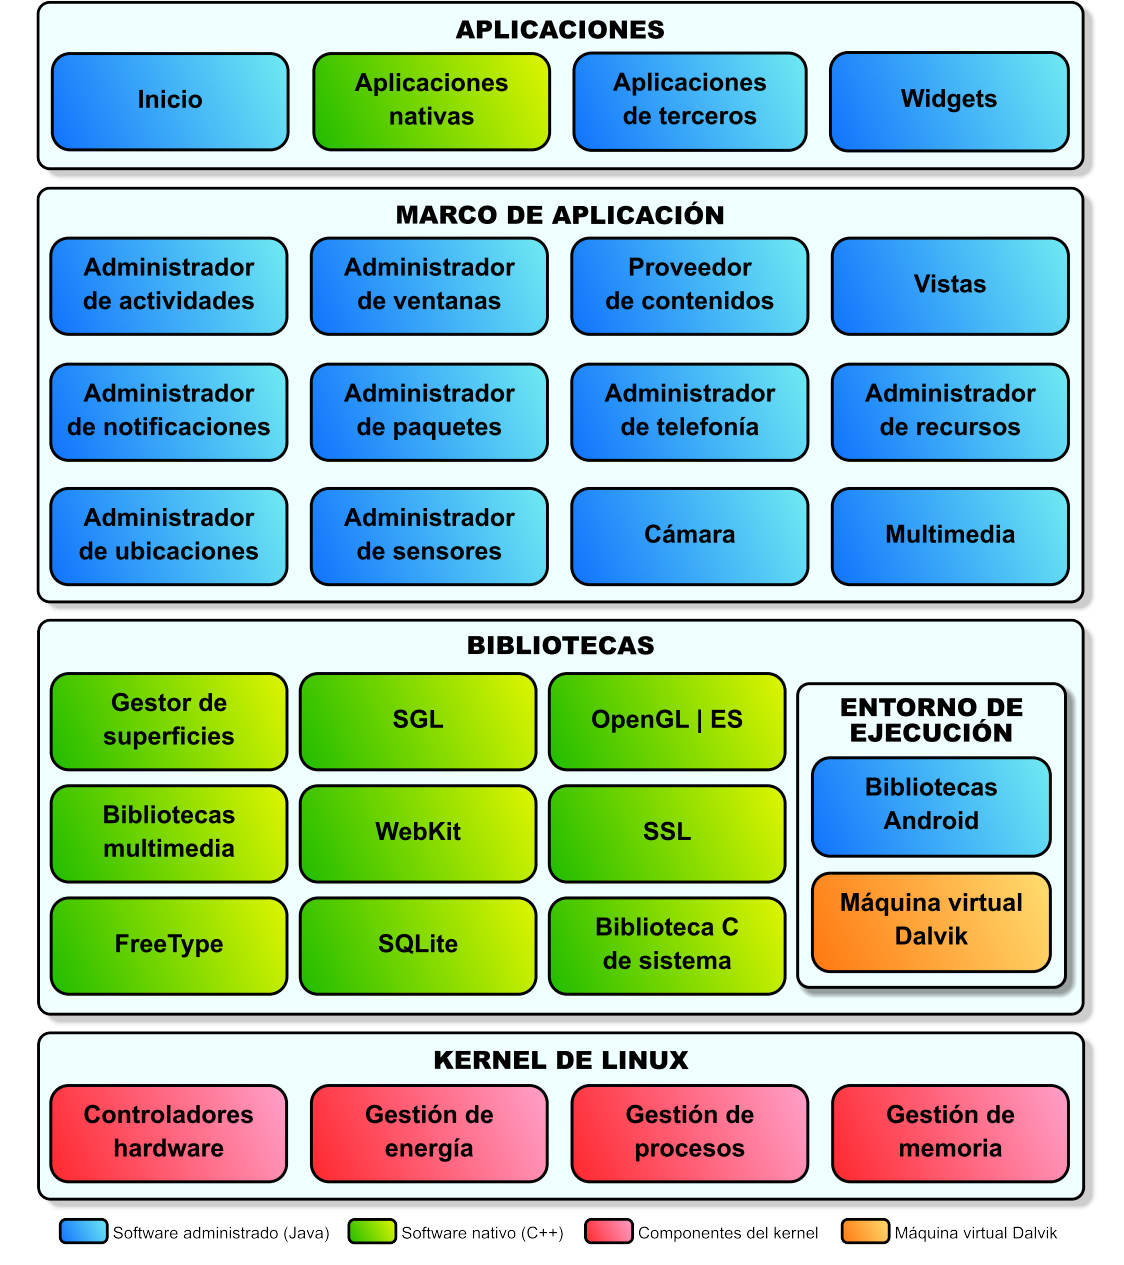
\includegraphics[width=12cm]{Imagenes/arquitectura_android}
\caption{Arquitectura de Android, compuesta por cuatro capas. \cite{15}}
\label{fig:Fig1}
\end{figure}

\item \textbf{Marco o Framework de Aplicaciones:} La tercera capa est� compuesta por todas las clases y servicios que se utilizan al momento de programar aplicaciones. Los compontentes que posee son:
\begin{itemize}
\item \textbf{Administrado de actividades (Activity Manager):} Gestiona la pila de actividades de la aplicaci�n, como tambi�n su ciclo de vida.

\item \textbf{Administrador de ventanas (Windows Manager):} Organiza lo que se mostrar� en pantalla. Crea las superficies en la pantalla, que posteriormente estar�n ocupadas por las actividades.

\item \textbf{Proveedor de contenidos (Content Provider):} Encapsula los datos que pueden ser compartidos por las aplicaciones, facilitando la comunicaci�n entre �stas.

\item \textbf{Vistas (Views):} Son los elementos que permiten construir las interfaces de usuario, como listas, botones, textos, hasta otros elementos m�s avanzados como visores de mapas.

\item \textbf{Administrador de notificaciones (Notification Manager):} Provee los servicios que notifican al usuario, mostrando alertas en la barra de estado. Tambi�n permite activar el vibrado, reproducir alertas de sonido y utilizar las luces del dispositivo.

\item \textbf{Administrador de paquetes (Package Manager):} Gestiona la instalaci�n de nuevos paquetes y adem�s permite obtener informaci�n sobre los que ya est�n instalados.

\item \textbf{Administrador de telefon�a (Telephony Manager):} Permite realizar llamadas, como tambi�n el env�o y recepci�n de SMS.

\item \textbf{Administrado de recursos (Resource Manager):} A trav�s de este administrador se podr� acceder a los elementos que no forman parte del c�digo, como im�genes, sonidos, layouts, etc. 

\item \textbf{Administrado de ubicaciones (Location Manager):} Permite obtener la posici�n geogr�fica actual del dispositivo a trav�s de GPS o redes.

\item \textbf{Administrado de sensores (Sensor Manager):} Permite la manipulaci�n de distintos sensores del dispositivo, como el aceler�metro, giroscopio, br�jula, sensor de proximidad, etc.

\item \textbf{C�mara:} Permite el uso de la c�mara del dispositivo para la obtenci�n de fotograf�as o v�deos.

\item \textbf{Multimedia:} Permite la visualizaci�n y reproducci�n de im�genes, v�deos y audio.

\end{itemize}

\item \textbf{Aplicaciones:} En esta capa se encuentran todas las aplicaciones del dispositivo, tanto las preinstaladas, como aquellas instaladas por el usuario. Tambi�n est� la aplicaci�n principal del sistema, el Inicio o launcher, desde donde se inician todas las aplicaciones.
\end{itemize}

\subsection{�C�mo las aplicaciones son compiladas?}
Al comenzar a desarrollar una aplicaci�n de Android, generalmente se crea un proyecto usando un IDE (Integrated Development Environment) como Eclipse o Android Studio. El proyecto contendr� c�digo fuente en Java y recursos. Cuando se compila el proyecto \cite[p.~14]{10} lo que ocurre es que se generan los Bytecode Java (archivos .class) en base al c�digo fuente Java (archivos .java). Luego se compilan estos archivos .class gener�ndose archivos ejecutables Dalvik (archivos .dex), los cuales pueden ser ejectuados por la m�quina virtual Dalvik que est� disponible en todos los dispositivos Android.\\

Al compilar un proyecto se colocan los archivos .dex y el resto de los archivos del proyecto en uno solo llamado APK (Android Package). Este contiene todos los archivos necesarios para ejecutar la aplicaci�n, incluyendo los .dex, recursos compilados, recursos sin compilar, y una versi�n binaria del Android Manifest.\\

El \textit{Android Manifest} es un archivo que especifica informaci�n esencial que el sistema debe tener antes de ejecutar la aplicaci�n. Toda aplicaci�n debe tener este archivo de forma no binaria en su proyecto.\\

Por razones de seguridad todas las aplicaciones de Android deben ser firmadas digitalmente con un certificado.\\

Finalmente el ADB (Android Debug Bridge) permiten que el IDE se comunique con un dispositivo f�sico de Android o un emulador.

\section{Tipos de dispositivos}
En el sitio web de Android \cite{1}, se pueden apreciar los dos tipos de dispositivos m�s populares de la plataforma, los smartphones y las tablets (Figura \ref{fig:Fig2}). Sin embargo, debido a que el c�digo de Android es de c�digo abierto, �ste puede ser personalizado para que funcione con otros tipos de dispositivos electr�nicos.

\begin{figure}[h!]
\centering
	    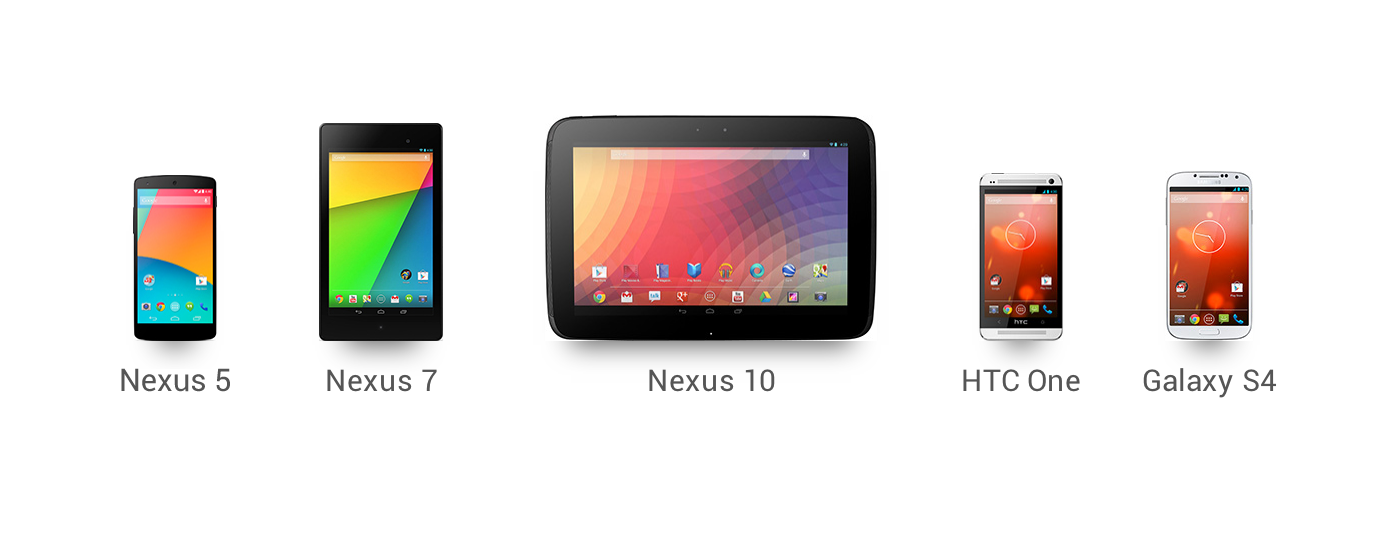
\includegraphics[width=12cm]{Imagenes/dispositivos_android}
\caption{�ltimos smartphones y tablets destacadas en el sitio de Android. \cite{1}}
\label{fig:Fig2}
\end{figure}

A continuaci�n se listan los otros dispositivos que cuentan con Android:\cite[p.~5]{10}
\begin{itemize}
\item Lectores de libros.

\item C�maras.

\item Sistemas en veh�culos.

\item Casas inteligentes.

\item Consolas de videojuegos.

\item Televisores inteligentes.

\item Relojes inteligentes.
\end{itemize}

\section{Versiones}
En la figura \ref{fig:Fig3} se detallan las distintas versiones que ha tenido Android. La primera versi�n comercial fue lanzada en Septiembre del 2008. Android est� bajo constante desarrollo por parte de Google y de la Open Handset Alliance, contando con un gran n�mero de actualizaciones desde su lanzamiento.\\

Desde Abril del 2009, los nombres de las versiones de Android han estado relacionados con postres y dulces, y adem�s han seguido un orden alfab�tico. El orden es Cupcake (1.5), Donut (1.6), Eclair (2.0-2.1), Froyo (2.2-2.2.3), Gingerbread (2.3-2.3.7), Honeycomb (3.0-3.2.5), Ice Cream Sandwich (4.0-4.0.4), Jelly Bean (4.1-4.3), y KitKat(4.4). El 3 de Septiembre del 2013, Google anunci� que exist�an un bill�n de dispositivos activos usando el sistema operativo Android en todo el mundo. La actualizaci�n m�s reciente de android fue KitKat 4.4, lanzado para dispositivos comerciales el 22 de Noviembre del 2013.
\begin{figure}[h!]
\centering
	    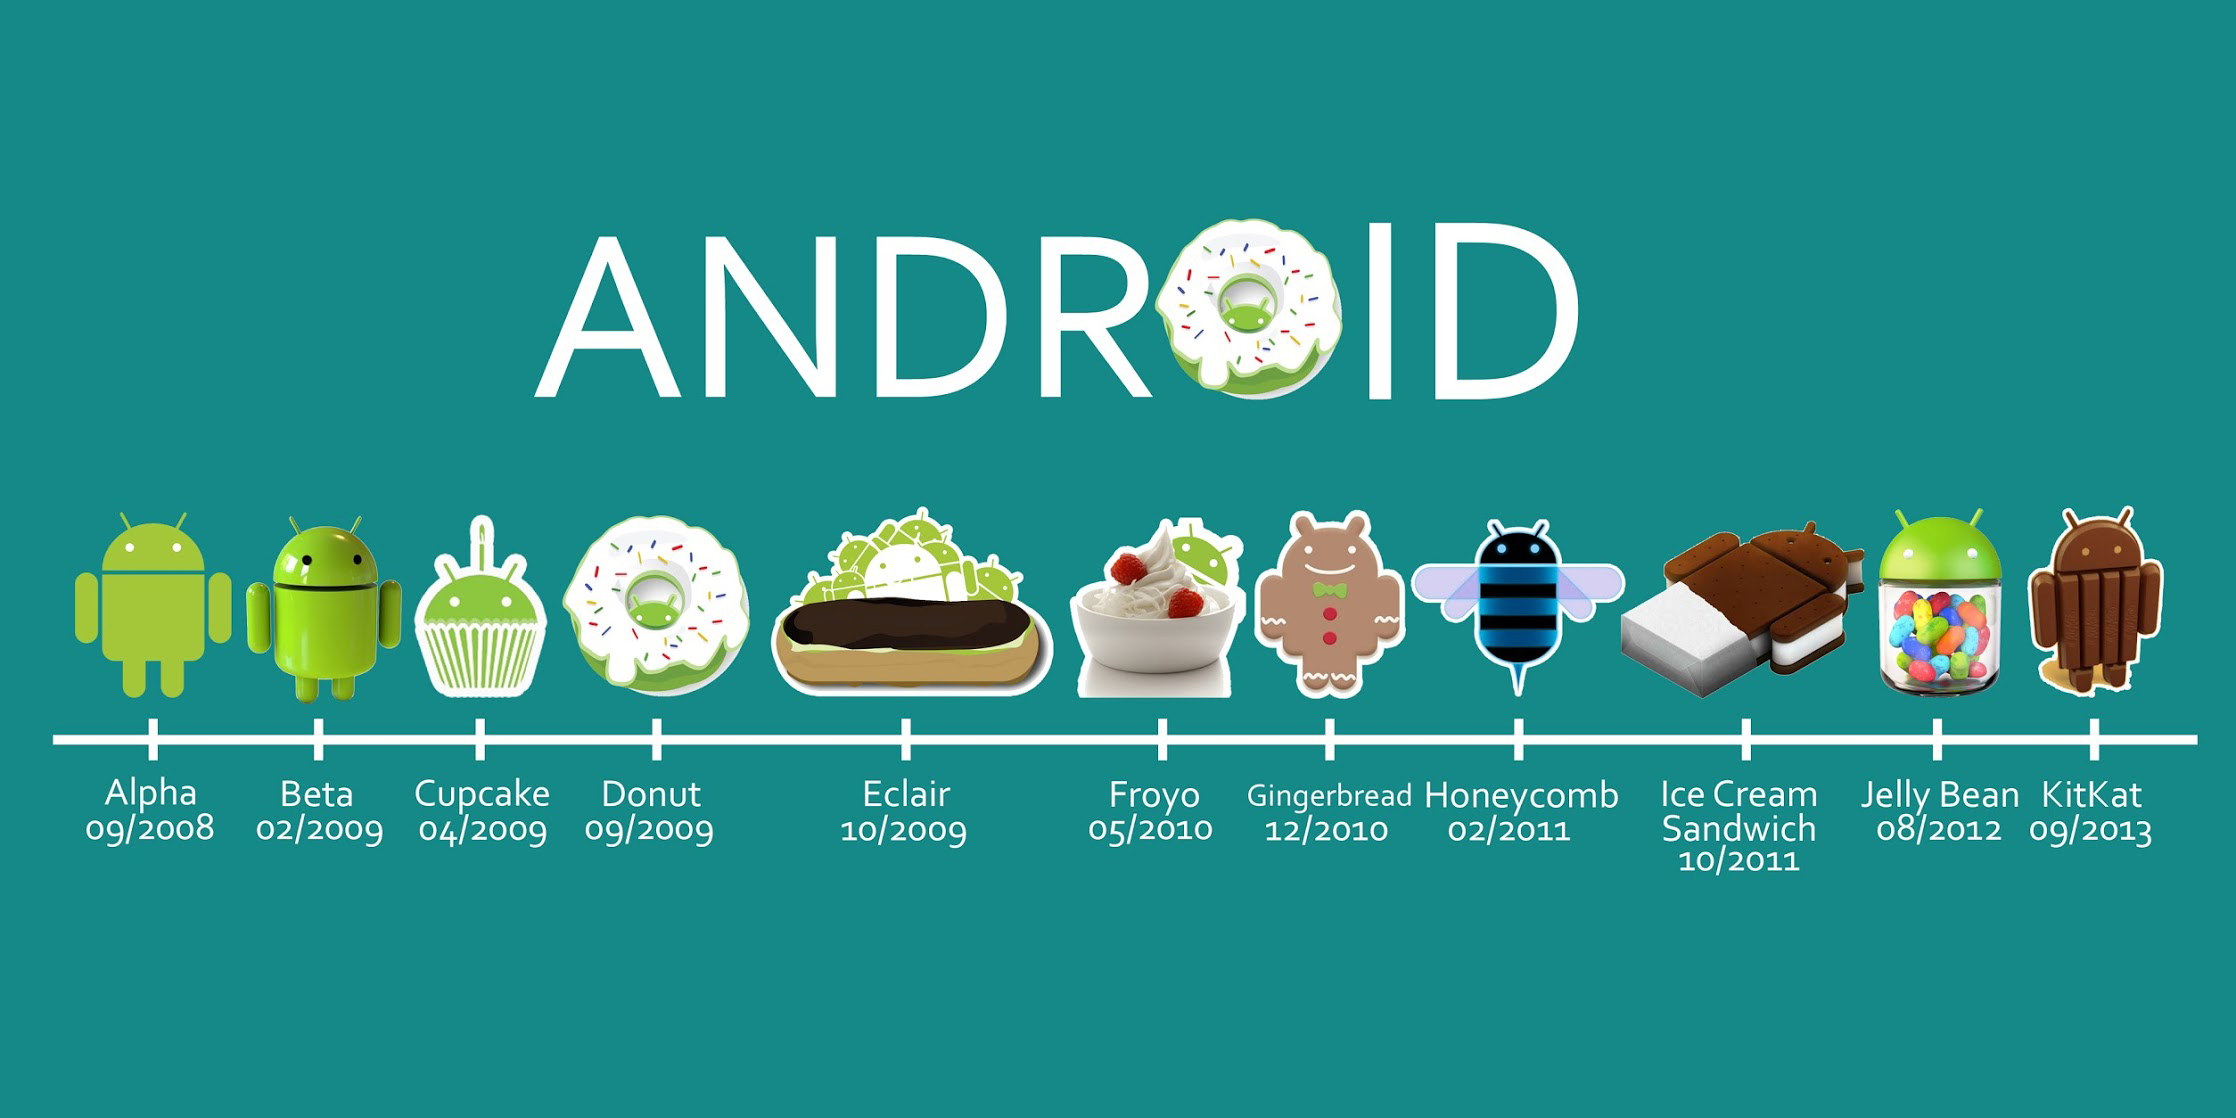
\includegraphics[width=14cm]{Imagenes/versiones_android}
\caption{Versiones de Android. \cite{16}}
\label{fig:Fig3}
\end{figure}

Al comenzar el desarrollo de una aplicaci�n Android, se debe decidir cu�l va a ser la API m�nima a la que se dar� soporte. Esto tendr� repercusiones al momento de que un usuario desee instalar la aplicaci�n, ya que si su dispositivo cuenta con una versi�n como Froyo o Eclair, lo m�s probable es que no pueda instalar pr�cticamente ninguna de las aplicaciones disponibles en Google Play, la tienda en que se encuentran todas las aplicaciones que suben los desarrolladores.\\

Android actualiza mes a mes las estad�sticas relativas al n�mero de dispositivos que tienen cada versi�n del sistema operativo \cite{2}. Esto ayuda a tener una gu�a sobre cu�l va a ser la API m�nima soportada. En la figura \ref{fig:Fig4} se muestran las estad�sticas correspondientes al mes de Abril. Esta informaci�n es recolectada durante los �ltimos 7 d�as de cada mes. Adem�s se ignoran las versiones que tienen menos de un 0.1\%. Se puede apreciar que el sistema operativo que hoy en d�a es dominante corresponde a Jelly Bean con m�s de un 60\%. El nuevo sistema operativo KitKat tiene s�lo un 5.3\% debido principalmente a que los operadores y fabricantes a�n no tienen listas sus versiones personalizadas de KitKat, en las que pueden incluir nuevas funcionalidades o quitar lo que estimen conveniente.\\
\begin{figure}[h!]
\centering
	    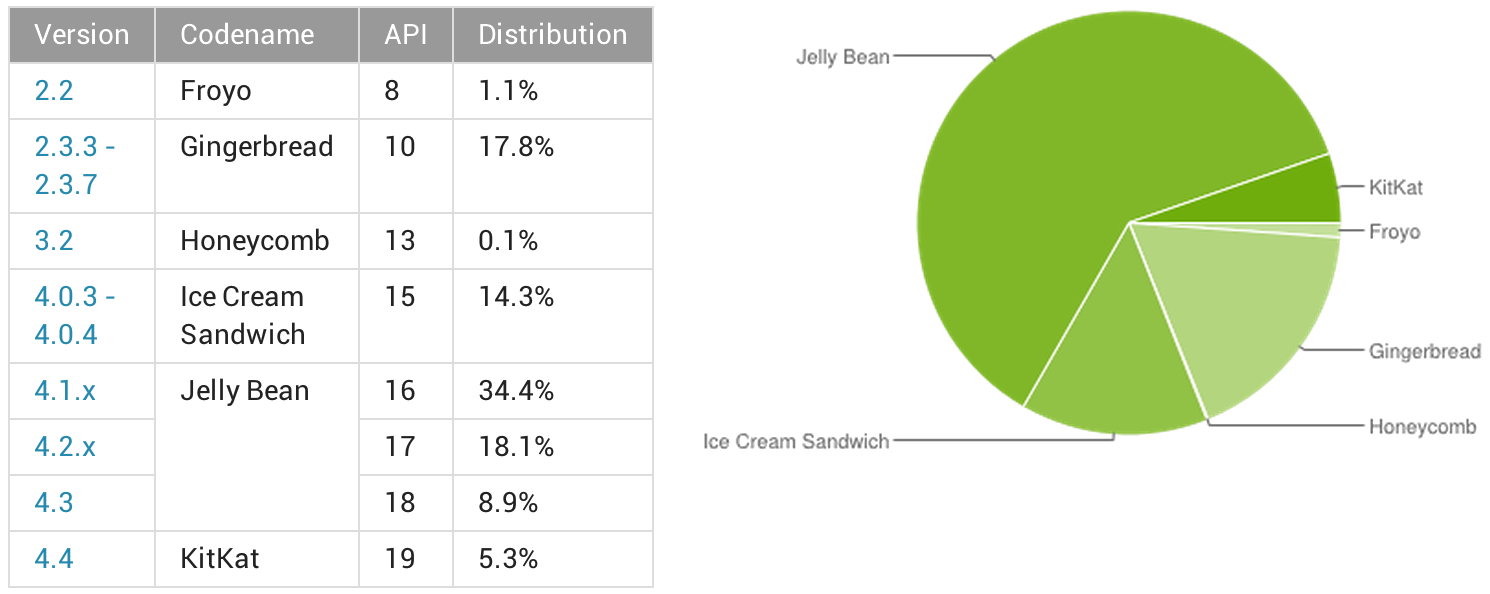
\includegraphics[width=14cm]{Imagenes/dashboard_android}
\caption{Estad�sticas relativas al n�mero de dispositivos que tiene cada versi�n de Android en Abril del 2014. \cite{2}}
\label{fig:Fig4}
\end{figure}

\section{Testing}
Con tantos dispositivos y sistemas operativos vigentes, asegurar la calidad de la aplicaci�n a trav�s de testing es un proceso vital y necesario, aunque tambi�n puede ser uno de los mayores dolores de cabeza para los desarrolladores. Lo que funciona perfectamente en un dispositivo, en otro puede no resultar como se espera. Es por ello que es absolutamente necesario el uso de herramientas que ayuden a reducir los riesgos inherentes de que una aplicaci�n sea compatible con m�s de 11.000 dispositivos distintos \cite{4}. A continuaci�n se dar�n a conocer los tipos de testing m�s conocidos.

\paragraph{Testing unitario}
\par Un test unitario (unit test) es una pieza de c�digo escrito por un desarrollador que ejecuta una funcionalidad espec�fica en el c�digo que va a ser testeado. Este tipo de test se enfoca en aislar un componente, por ejemplo un m�todo o una clase, para ser capaces de testearlo de forma replicable. Es por esto que los test unitarios y los objetos simulados (mock objects) normalmente se usan en forma conjunta. Estos objetos simulados se usan para poder repetir el test innumerables veces. Por ejemplo, si se quisiera testear el momento en que se borra informaci�n desde una base de datos, probablemente no se quiere que los datos realmente se borren y que la pr�xima vez que se desee testear, �stos ya no se encuentren.\\

Los test unitarios aseguran que el c�digo funcione como se espera. Tambi�n son muy �tiles para asegurar que el c�digo sigue funcionando correctamente despu�s de hacer cambios en otras partes del proyecto, al momento de arreglar bugs o a�adir nuevas funcionalidades.

\paragraph{Testing de User Interface (UI)}
\par Adem�s de testear los componentes individuales que permiten el funcionamiento de la aplicaci�n, como actividades y servicios, es muy importante testear el comportamiento de la interfaz de la aplicaci�n cuando est� en funcionamiento en un dispositivo. El testing de UI asegura que la aplicaci�n se comportar� de forma correcta en respuesta de acciones que realice el usuario en un dispositivo, tales como escribir en el teclado, presionar botones o im�genes, entre otros controles. Se debe tener consideraci�n especial con los test que involucran elementos de UI, ya que �nicamente la hebra principal tiene permisos para alterar la UI en Android.\\

Un estrategia com�n es testear de forma manual la UI, verificando que la aplicaci�n se comporta como se espera al realizar una serie de acciones. Sin embargo, este enfoque puede consumir mucho tiempo y ser bastante tedioso, como tambi�n, se pueden pasar por alto algunos errores. Un m�todo m�s eficiente y confiable ser�a automatizar el testing de la interfaz con algun framework que facilite esta tarea.

\paragraph{Testing de integraci�n}
\par Los test de integraci�n est�n dise�ados para testear el comportamiento que los componentes individuales tienen cuando funcionan de forma conjunta. Esto normalmente se realiza una vez que ya se han aprobado los test unitarios. Adem�s tienden a ser m�s complejos y lentos que los test unitarios.

\paragraph{Testing funcional o de aceptaci�n}
\par Normalmente estos tipos de test son creados por profesionales del �rea de negocios y de control de calidad. Adem�s son expresados en un lenguaje de negocios. Estos son test de alto nivel para testear el correcto funcionamiento de los requierimientos o caracter�sticas que deber�a tener la aplicaci�n. Los testers y desarrolladores tambi�n pueden colaborar en la creaci�n de �stos. 

\paragraph{Testing de sistema}
\par El sistema es testeado como un todo, y la interacci�n entre los componentes, software y hardware es testeada. Normalmente, los test de sistema incluyen:
\begin{itemize}

\item Smoke test: Es un testing r�pido que se lleva a cabo sobre toda la aplicaci�n. Su objetivo no consiste en encontrar bugs, sino que asegurar que las funcionalidades b�sicas se comportan de manera correcta.

\item Test de desempe�o: Los test de desempe�o miden alguna caracter�stica de un componente en una forma replicable. Si se necesitan mejoras en el desempe�o de alg�n componente de la aplicaci�n, el mejor enfoque es medir el desempe�o antes y despu�s de la inclusi�n de un cambio. De esta forma se entiende claramente el impacto que ha tenido el cambio en el desempe�o.
\end{itemize}

La lista anterior describe los posibles tests que hoy en d�a existen para asegurar la calidad de las aplicaciones m�viles, pero tan importante como saber hacer testing, es saber qu� cosas son necesarias testear. A continuaci�n se listan algunas situaciones com�nes relacionadas con Android que se deber�an tener en cuenta al momento de testear.
\paragraph{Cambios de orientaci�n}
Para dispositivos que soportan m�ltiples orientaciones, Android detecta los cambios de orientaci�n cuando el usuario rota el dispositivo, dej�ndolo en \textit{landscape} (posici�n horizontal) en vez de \textit{portrait} (posici�n vertical).\\

Cuando ocurre esto, el comportamiento por defecto es destruir y recomenzar la Activity. Se deber�an tener en cuenta las siguientes preguntas:
\begin{itemize}
\item �Se dibuja de forma correcta la pantalla?

\item �La aplicaci�n mantiene el estado? La Activity no deber�a perder nada que el usuario haya ingresado en la UI.
\end{itemize}

\paragraph{Cambios de configuraci�n}
Tambi�n pueden ocurrir otros cambios m�s generales en el sistema, como un cambio de idioma. Este tipo de cambios desencadena el comportamiento por defecto de destruir y recomenzar la Activity. 

\paragraph{Dependencias de fuentes externas}
Si la aplicaci�n depende de acceso a internet, o usa GPS, entonces se deber�a testear qu� pasa cuando estos recursos no est�n disponibles.

\paragraph{Cambios en segundo plano}
Si la aplicaci�n est� inactiva y ya ha pasado a segundo plano, lo m�s probable es que el sistema destruya la o las Activities de la aplicaci�n para dar memoria a otras aplicaciones que esten corriendo actualmente. Es por ello que es necesario testear el ciclo de vida de la Activity para corroborar si se destruye y recomienza de forma exitosa, sin p�rdida del estado actual.

Para el caso de testing de clases en aplicaciones Android, es posible que ocurran dos casos: que las clases realicen llamadas a la API de Android o que s�lamente usen c�digo Java.

\paragraph{Testing de clases en Java \cite{19}}
\par Si las clases que se tienen no hacen llamadas a la API de Android, se puede usar el framework de JUnit sin ning�na restricci�n.

La ventaja de este m�todo es que se puede usar cualquier framework de testing que sea para Java y la velocidad con que se ejecutan los tests deber�a ser mucha m�s r�pida comparada con los tests que requieren de un sistema con Android.

\paragraph{Testing de clases en Java que usan la API de Android \cite{19}}
\par Si se quieren hacer tests que usen la API de Android, �stos necesitan llevarse a cabo en un dispositivo con Android. Esto hace que la ejecuci�n de los tests tome m�s tiempo, principalmente porque el archivo \textit{android.jar} no contiene el c�digo del framework de Android. Este archivo es �nicamente usado al momento de compilar una aplicaci�n. Una vez que la aplicaci�n est� instalada, se utilizar� el \textit{android.jar} que est� en el dispositivo.



\section{Problemas al desarrollar en Android}
Ahora que ya se han dado a conocer aspectos b�sicos sobre Android, se puede profundizar en los problemas m�s com�nes que se enfrentan al desarrollar aplicaciones.\\
\subsection{Fragmentaci�n}
La Fragmentaci�n es el elemento que m�s afecta a Android. Debido a los m�s de 11.000 diferentes tipos de dispositivos \cite{4}, como tambi�n a las ocho versiones vigentes del sistema operativo \cite{2}, es mucho m�s dif�cil desarrollar una aplicaci�n robusta y estable, ya que es pr�cticamente imposible poder probar la aplicaci�n en todas las combinaciones de dispositivos y software existentes. Es posible clasificar la fragmentaci�n en dos categorias, a trav�s de las cuales desembocan la mayor�a de los problemas que un desarrollador debe enfrentar: software y hardware.
\subsubsection{Fragmentaci�n a nivel de software}
Como ya se mencion� anteriormente, existen muchas versiones del sistema operativo Android vigentes hoy en d�a. Esto priva al desarrollador de m�todos �tiles al momento de programar su aplicaci�n, ya que se debe establecer una API m�nima. En base a las estad�sticas que provee Android, la mayor�a de los desarrolladores decide dar soporte desde Gingerbread en adelante. Si el desarrollador desea utilizar m�todos de una API superior a la de Gingerbread, debe especificar en el c�digo fuente que esa parte s�lo tiene que ser ejecutada si el dispositivo del usuario es mayor o igual a la API 11. La siguiente porci�n de c�digo \cite{11} es un ejemplo de lo que los desarrolladores deben hacer: \\
\begin{lstlisting}
if (Build.VERSION.SDK_INT > Build.VERSION_CODES.GINGERBREAD_MR1) {
    // Aqu� va c�digo superior a la API 10 de Gingerbread
}
\end{lstlisting}
Esto provoca muchas veces que el desarrollador deba programar una funcionalidad m�s de una vez. Actualmente varios desarrolladores est�n optando por dar soporte a sus aplicaciones desde Ice Cream Sandwich en adelante, debido principalmente a la gran recepci�n que ha tenido Jelly Bean y a la ca�da constante que est� teniendo Gingerbread. Si se toma en cuenta que este �ltimo sistema operativo fue lanzado el a�o 2010 \cite{12} y a�n cuenta con cerca de un 20\%, se puede apreciar claramente el nivel de fragmentaci�n que existe, principalmente por la r�pidez con la que Android ha estado mejorando su sistema operativo, lanzando aproximadamente una nueva versi�n cada a�o.\\

A continuaci�n, en el gr�fico de la figura \ref{fig:Fig5} se puede ver la distribuci�n hist�rica de versiones que ha tenido Android con el pasar de los a�os. Si bien se visualiza que a�n existe una gran fragmentaci�n, esto ha ido disminuyendo y Android cada vez se est� convirtiendo en un sistema operativo m�s estable y maduro. Por ejemplo, si se compara el porcentaje que ten�a Gingerbread en el a�o 2013 (39.8\%) con el de este a�o (17.8\%) se ve que hay una diferencia sustancial, y gran parte de este porcentaje se ha trasladado a Jelly Bean, que el a�o pasado contaba con un 25\% del mercado y hoy en d�a cuenta con m�s del 60\%.\\
\begin{figure}[h!]
\centering
	    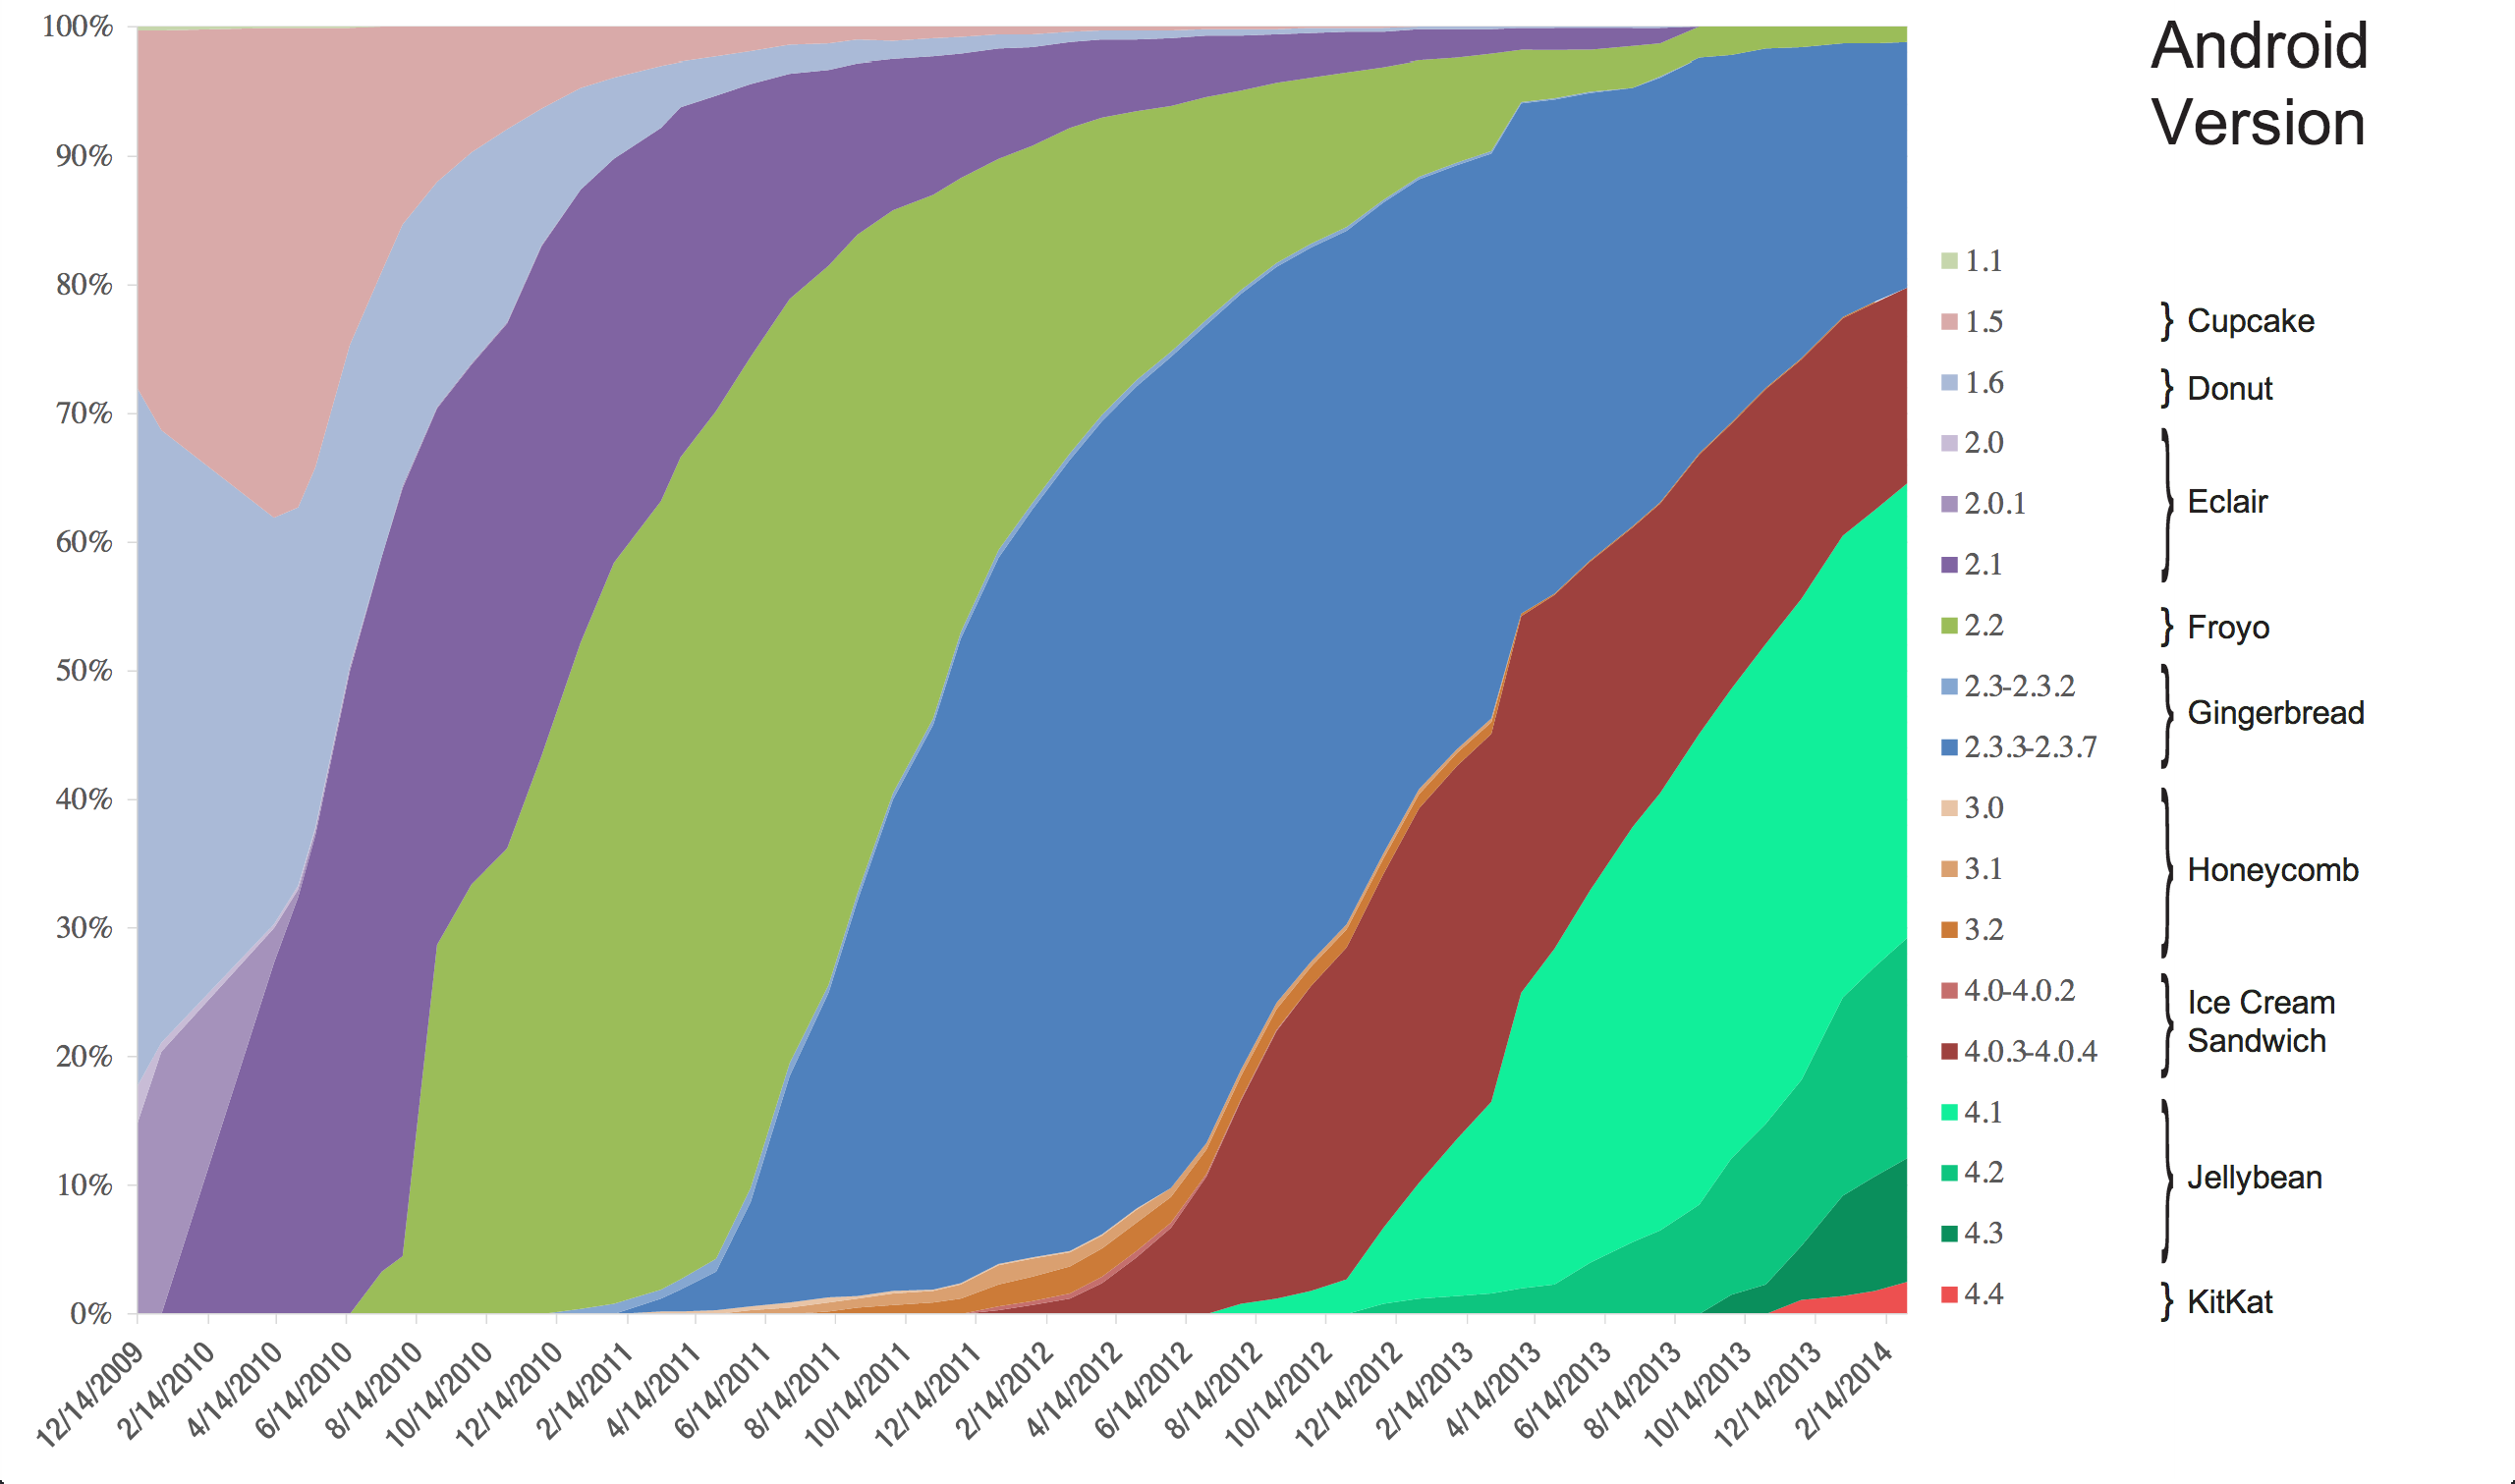
\includegraphics[width=14cm]{Imagenes/historical_progress_android}
\caption{Distribuci�n hist�rica de versiones de Android.\cite{13}}
\label{fig:Fig5}
\end{figure}
\par
Muchas veces los crashes y errores en los que la aplicaci�n deja de funcionar correctamente, ocurren en un sistema operativo m�s antiguo y ya fueron arreglados en los sistemas operativos m�s nuevos. Esto ocasiona que al probar la aplicaci�n en un smartphone como un Nexus 4 o como un Samsung S3, no ocurran problemas que si podr�an verse en dispositivos m�s antiguos.  Adem�s, debido a que a veces los operadores o fabricantes no ofrecen actualizaciones al sistema actual, el dispositivo no es actualizado, por lo que estos errores persistir�n.

\subsubsection{Fragmentaci�n a nivel de hardware}
Este tipo de fragmentaci�n es la que m�s afecta a los desarrolladores. Por un lado, la gran cantidad de dispositivos es la que ha permitido la r�pida evoluci�n de Android, ya que cualquier fabricante puede adaptar el sistema operativo a sus necesidades e incluirlo en su hardware. Para los desarrolladores, este tipo de fragmentaci�n es la que genera m�s pesadillas, pues cada dispositivo con Android cuenta con diferentes caracter�sticas. A continuaci�n se detallan los problemas derivados por la fragmentaci�n de hardware.
\paragraph{Fragmentaci�n en los tama�os de pantalla}
Existen cuatro tama�os generales de pantallas \cite{2}: peque�a (small), normal, grande (large) y extra grande (xlarge). Para optimizar la experiencia del usuario, muchas veces se debe implementar una interfaz distinta para un tipo espec�fico de pantalla. Esto se lleva a cabo a trav�s de un archivo llamado layout, escrito en XML que define los elementos presentes en la interfaz.\\

Si se desea usar el mismo layout para todas las pantallas simplemente se deben ir guardando estos archivos en la carpeta de recursos del proyecto, \textit{res/layout}. En caso que se quiera agregar un layout distinto para un tipo de pantalla, adem�s de tener un archivo en la ruta antes mencionada, se debe crear una nueva carpeta de layouts, a�adiendo el sufijo que corresponda a cada tama�o de pantalla. \\

\begin{figure}[h!]
\centering
      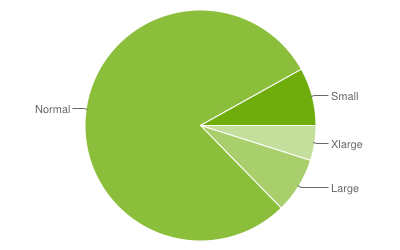
\includegraphics[width=8cm]{Imagenes/chart_screen_sizes}
\caption{Gr�fico con la distribuci�n de tama�os de pantalla durante el mes de Abril del 2014. \cite{1}, }
\label{fig:Fig6}
\end{figure}
Por ejemplo, si se quisiera agregar un layout distinto para pantallas grandes (large), se debe a�adir un archivo de layout a la carpeta \textit{res/layout-large}, por lo que existir�n dos versiones de este archivo, uno en la carpeta antes se�alada, mientras que el otro estar� en la carpeta general de layouts, \textit{res/layout}.\\

En el sitio web de Android \cite{1}, se entregan estad�sticas mensuales sobre el porcentaje de dispositivos que tiene cada tama�o de pantalla. En el gr�fico de la figura \ref{fig:Fig6} se muestra la distribuci�n de tama�os de pantalla durante el mes de Abril del 2014.

\paragraph{Fragmentaci�n en las resoluciones de pantalla}
Android categoriza las resoluciones de cada pantalla en base a la densidad de pixeles que poseen. Existen cinco tipos de densidades \cite{2}: baja (ldpi), media (mdpi), alta (hdpi), extra-alta (xhdpi) y extra-extra-alta (xxhdpi). Adem�s existe otro tipo de densidad, la cual es usada principalmente para televisores (tvdpi).\\

Muchas veces es necesario agregar diferentes versiones del mismo recurso gr�fico. Por ejemplo, si s�lo se agrega un recurso gr�fico en la resoluci�n m�s alta (xxhdpi), este probablemente se ver� bien en resoluciones altas como xxhdpi y xhdpi, pero para las m�s bajas, como hdpi o mdpi, la imagen ser� redimensionada y se perder� mucha calidad.\\

Al agregar elementos de UI como botones, textos, tablas, entre otros, tambi�n se debe considerar la densidad de pixeles, ya que si el ancho y alto se asignan en pixeles, va a ocurrir lo que se muestra en la figura \ref{fig:Fig7}. Por ello, es muy importante asignar valores que est�n en la escala de densidad de pixeles. 

\par
\begin{figure}[h!]
\centering
      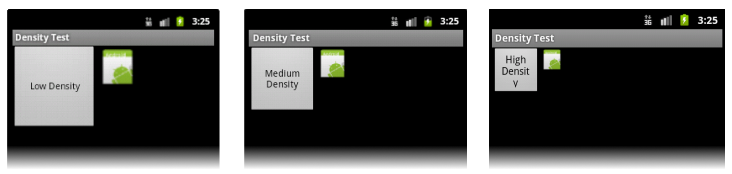
\includegraphics[width=14cm]{Imagenes/density_test_bad}
\caption{Consecuencias de asignar alto y ancho en pixeles en vez de en densidad de pixeles.\cite{17} }
\label{fig:Fig7}
\end{figure}

A�n con estas precauciones, es muy dif�cil saber cu�les son los valores de alto y ancho adecuados que deben ser asignados. Esto se debe a que existe una gran diferencia entre cada tipo de resoluci�n, ya que si por ejemplo se asignara a un elemento un ancho de 350dp, no existir�n problemas en una pantalla con una resoluci�n alta como un Nexus 4 (xhdpi), pues el elemento tomar�a un espacio de 700px, pero para un dispositivo con resoluci�n m�s baja como un Samsung Galaxy Young (ldpi) si existir�an, ya que el elemento tomar�a 262.5px y el ancho de la pantalla de este dispositivo es de 240px. A trav�s del siguiente sitio \cite{3}, se puede saber c�al es la densidad de pixeles de pr�cticamente todos los dispositivos m�s populares de Android.

En el gr�fico de la figura \ref{fig:Fig8} se puede apreciar la informaci�n que entrega Google sobre la distribuci�n de densidad existente durante el mes de Abril del 2014 \cite{1}.
\par
\begin{figure}[h!]
\centering
      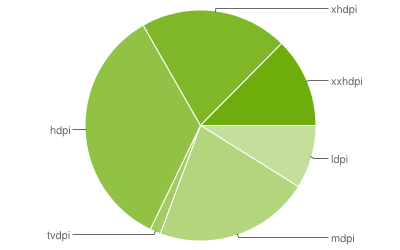
\includegraphics[width=8cm]{Imagenes/chart_density_pixels}
\caption{Gr�fico con la distribuci�n de densidades de pantalla durante el mes de Abril del 2014.\cite{13}}
\label{fig:Fig8}
\end{figure}
\subsubsection{Fragmentaci�n en otras caracter�sticas}
Adem�s de los tama�os de pantalla y sus resoluciones, existen otras caracter�sticas muy importantes que los desarrolladores deben tener en cuenta. Una de las principales es la RAM con la que cuenta el dispositivo, ya que es all� donde se cargan las instrucciones que ejecuta el procesador. Tambi�n es muy importante el procesador y la cantidad de n�cleos con los que cuenta. Aunque la mayor�a de los dispositivos tiene c�mara, tambi�n se debe tener en cuenta que algunos no la tiene. Por �ltimo, muchas veces los fabricantes como Samsung, hacen cambios en el sistema operativo, cambiando cosas nativas, lo cual produce diferentes experiencias en cada dispositivo, y muchas veces genera errores que el desarrollador no se espera.

\subsubsection{Reporte sobre Fragmentaci�n}
La compa��a \textit{OpenSignal} ha entregado dos reportes sobre la fragmentaci�n en Android en los a�os 2012 \cite{14} y 2013 \cite{4}. 
En su �ltimo reporte de Julio del 2013 se entregan gr�ficas que ayudan a visualizar el n�mero de dispositivos existentes. Estas gr�ficas se basan en 682.000 dispositivos �nicos que descargaron la aplicaci�n de OpenSignal. La raz�n de elegir este n�mero de dispositivos es porque se quer�a hacer una comparaci�n justa con respecto al reporte entregado el a�o 2012, en el que tambi�n se hab�a tomado una muestra de 682.000 dispositivos.

 En la gr�fica de la figura \ref{fig:Fig9} se apreciar los 11.868 dispositivos distintos que han descargado la aplicaci�n de \textit{OpenSignal} en los �ltimos meses. En su reporte del a�o 2012 este n�mero era de 3.997. En el sitio web \cite{4} se menciona lo siguiente:
\begin{quote}
\textit{``Esta es la mejor forma de visualizar realmente el n�mero de diferentes dispositivos Android que han descargado la aplicaci�n de OpenSignal en los �ltimos meses. Desde el punto de vista de un desarrollador, comparando la fragmentaci�n de este a�o con el anterior, hemos visto que se ha triplicado, con dispositivos incluso m�s raros de todas partes del mundo. Si se quiere entender el desafio de crear una aplicaci�n que funcione con todos los dispositivos que pueden descargarla, esta imagen es un buen punto para comenzar!"}
\end{quote}
\begin{figure}[h!]
\centering
      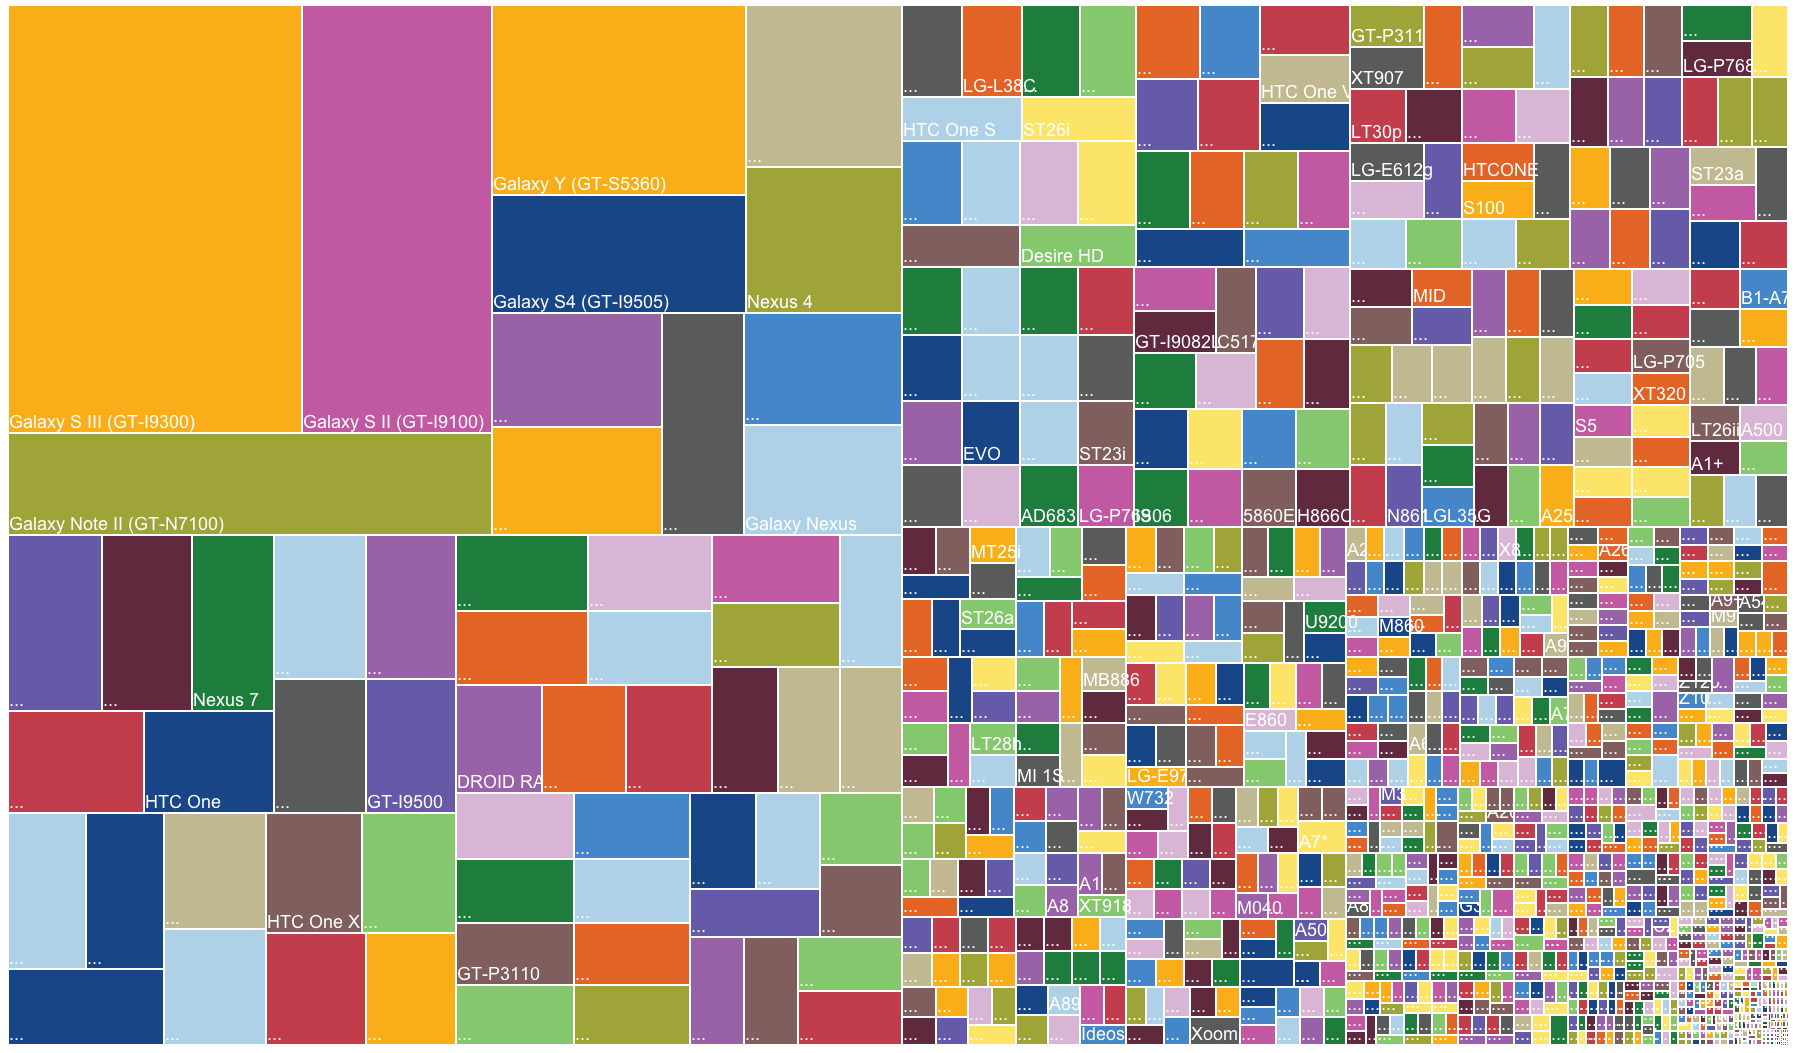
\includegraphics[width=12cm]{Imagenes/open_signal_dispositivos}
\caption{Fragmentaci�n de dispositivos entregado por OpenSignal el 2013. \cite{4}}
\label{fig:Fig9}
\end{figure}
Similar a las estad�sticas de dispositivos, la gr�fica de la figura \ref{fig:Fig12} muestra el porcentaje de mercado que maneja cada uno de los fabricantes. Se puede ver a Samsung claramente sobre el resto, con un 47.5\% del mercado. Sony se encuentra en la segunda posici�n con un 6.5\%, menos de un s�ptimo de lo que tiene Samsung. Algunas otras marcas que se encuentra en esta gr�fica, pero que tienen porcentajes muy bajos son Motorola, HTC, Huawei, LG y Google.
\begin{figure}[h!]
\centering
      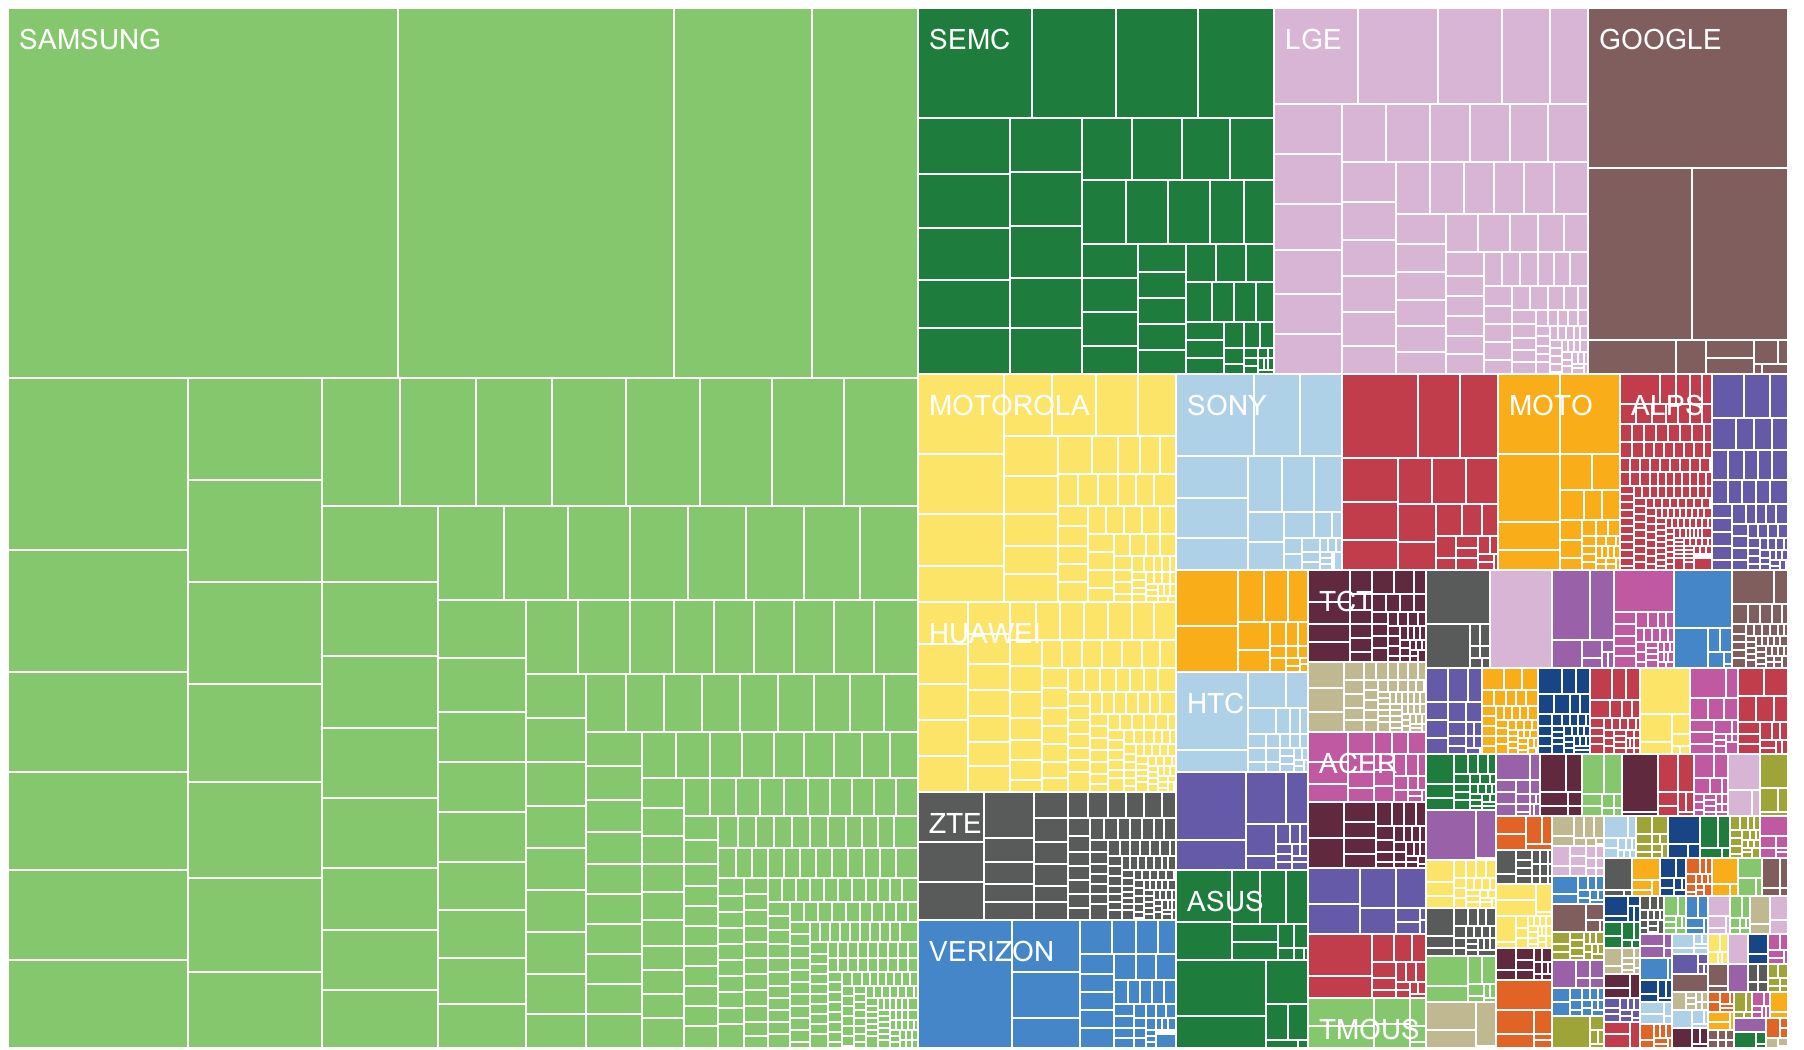
\includegraphics[width=12cm]{Imagenes/open_signal_branding}
\caption{Fragmentaci�n a nivel de fabricantes de dispositivos Android entregado por OpenSignal el 2013. \cite{4}}
\label{fig:Fig12}
\end{figure}
\par
Con respecto a los tama�os de pantallas, se menciona que la clave del �xito para cualquier aplicaci�n es tener una buena interfaz, y en este aspecto Android presenta dos desafios para los desarrolladores. Primero, los fabricantes tienden a producir sus propias variantes en la interfaz del usuario, cambiando el aspecto de varios elementos nativos de Android, como botones, switchs, listas, entre otros, por lo que no se puede entregar la misma experiencia a todos los usuarios a menos que se hagan cambios profundos para personalizar la interfaz. El otro desaf�o tiene relaci�n con los tama�os de pantalla, ning�n otro sistema operativo m�vil tiene tanta diversidad. En las figuras (\ref{fig:Fig10} y \ref{fig:Fig11}) se incluye una comparaci�n entre los tama�os de pantalla de los dispositivos Android en contraste con los de iOS. Las l�neas m�s oscuras representan la frecuencia de estas pantallas. Se hace �nfasis en que en la gr�fica lo que se muestra son los tama�os de pantalla f�sica, no los tama�os en pixeles.
\begin{figure}[h!]
\centering
      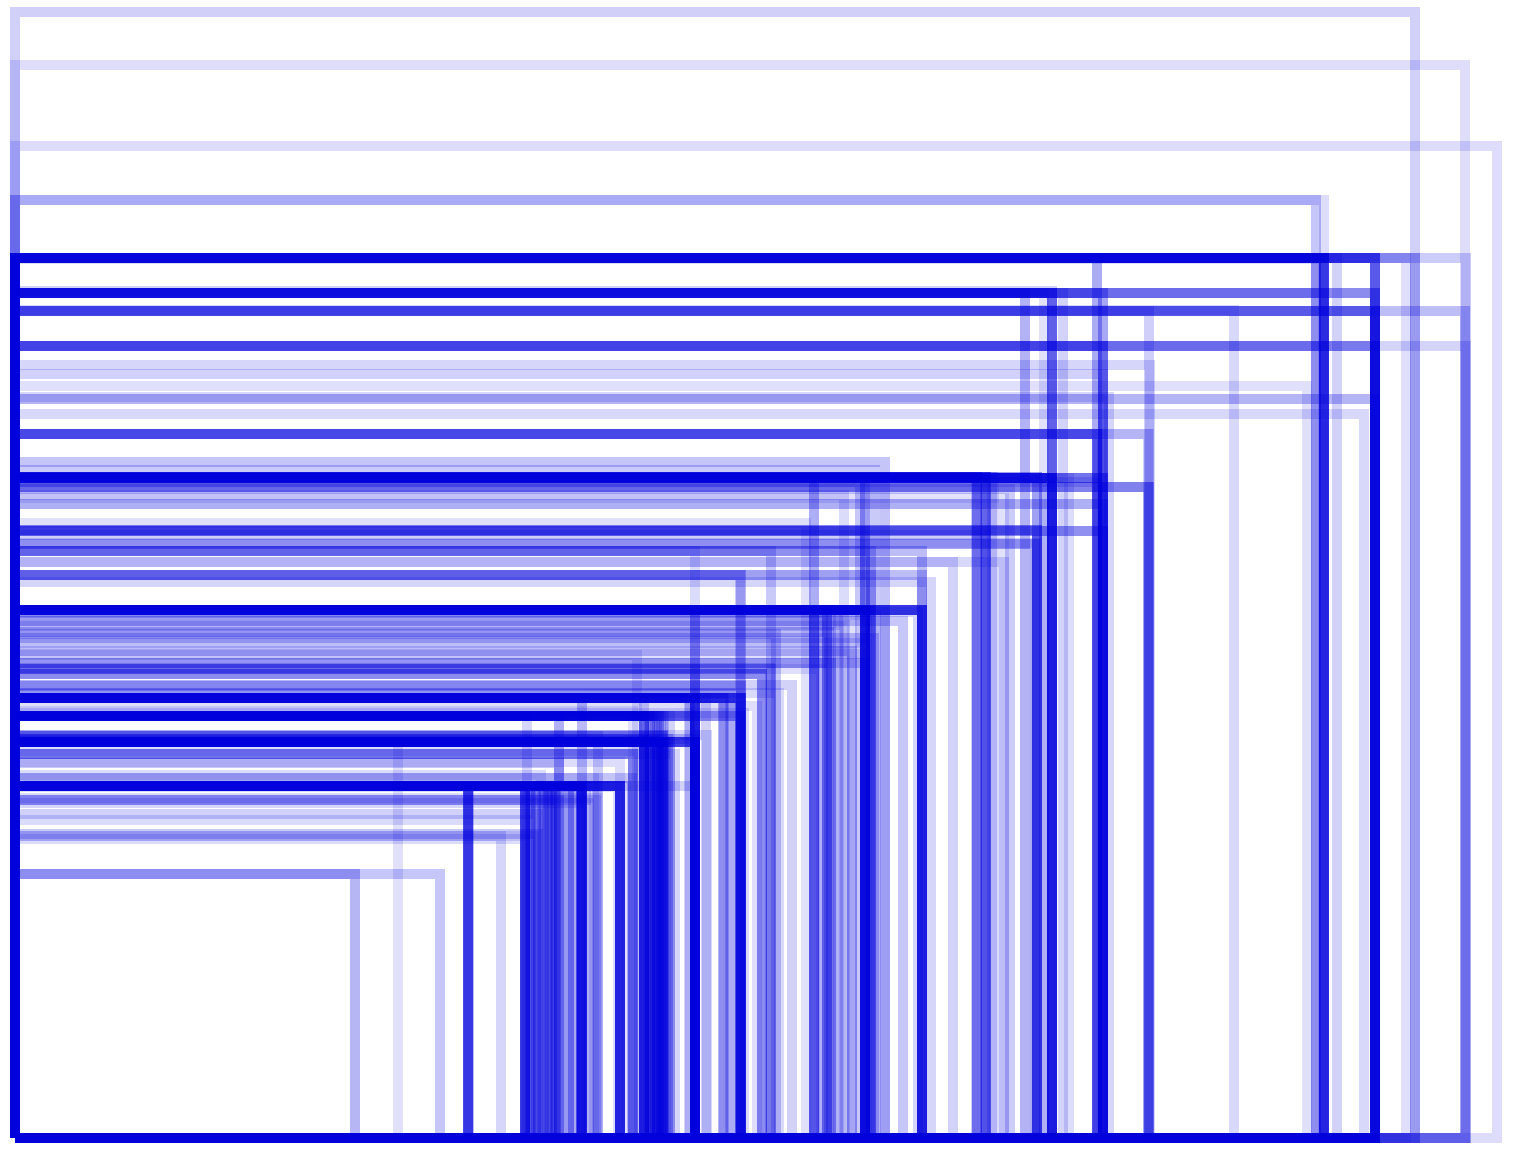
\includegraphics[width=12cm]{Imagenes/open_signal_tamanos_pantalla_android}
\caption{Fragmentaci�n de pantallas en dispositivos Android entregado por OpenSignal en Julio del 2013. \cite{4}}
\label{fig:Fig10}
\end{figure}

\begin{figure}[h!]
\centering
      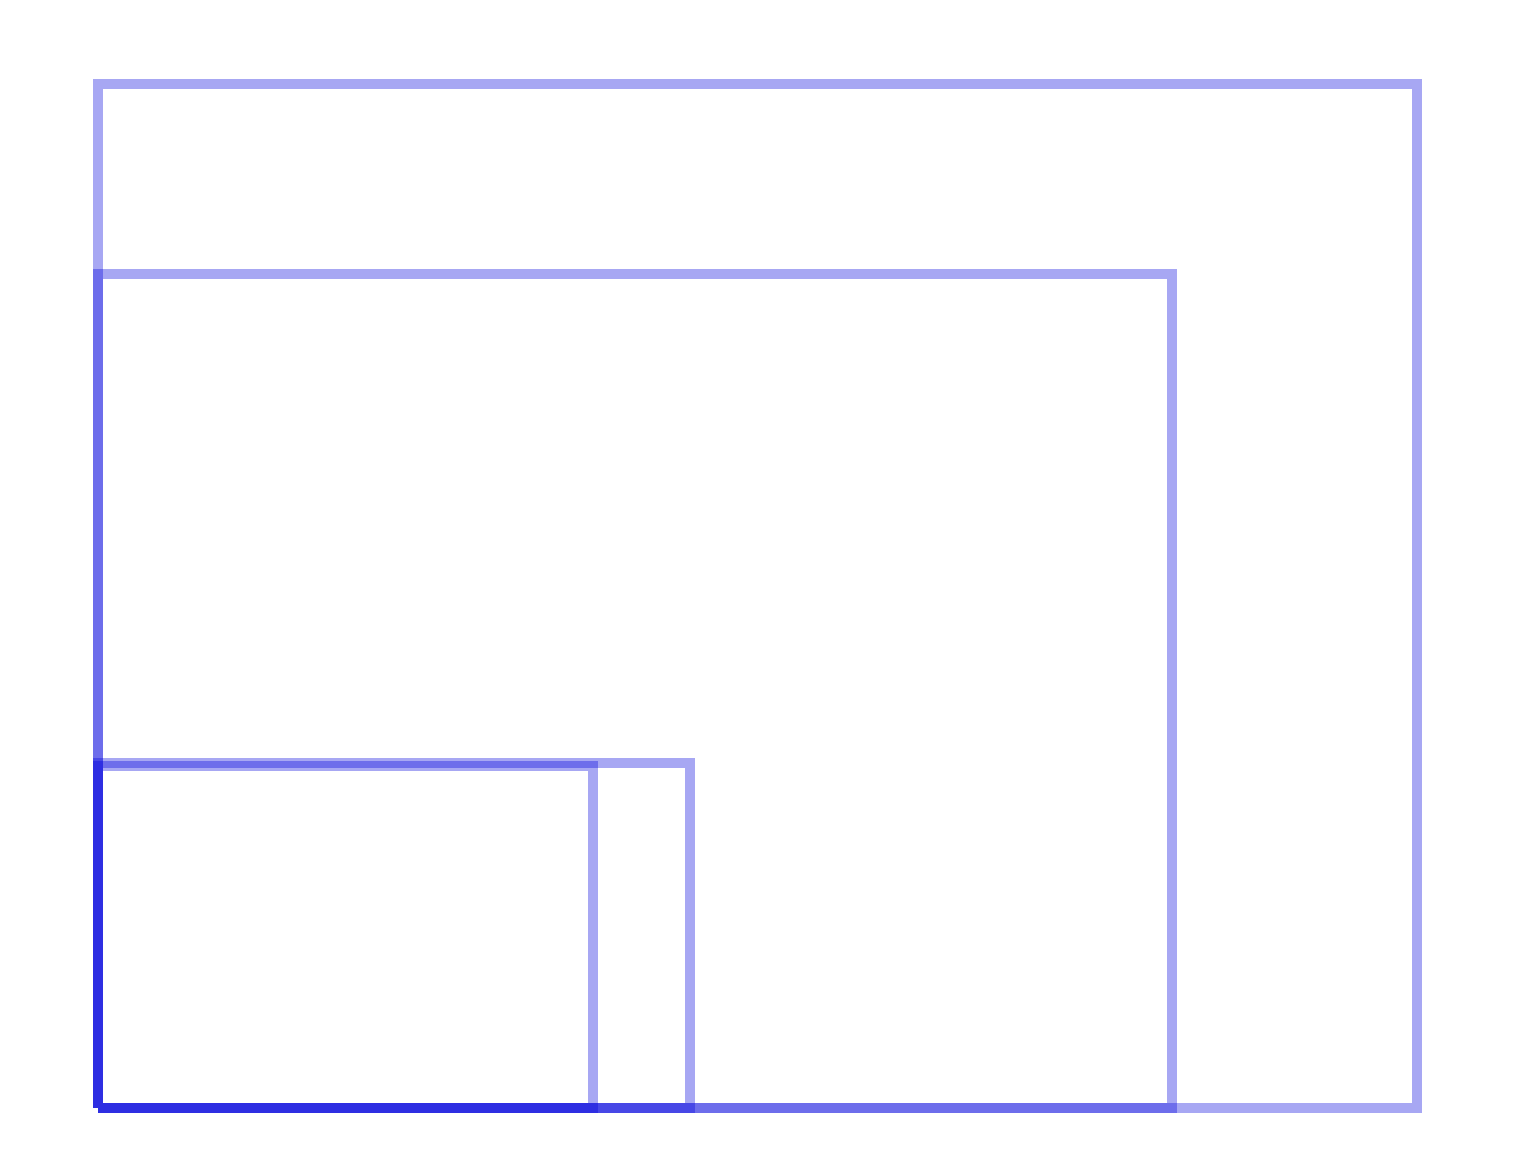
\includegraphics[width=12cm]{Imagenes/open_signal_tamanos_pantalla_ios}
\caption{Fragmentaci�n de pantallas en dispositivos iOS entregado por OpenSignal en Julio del 2013. \cite{4}}
\label{fig:Fig11}
\end{figure}

\subsection{Distribuci�n de versiones Alpha y Beta}
Durante el proceso de desarrollo de una aplicaci�n, normalmente se compilan versiones Alpha y Beta, las cuales son versiones que no son las finales, por lo que se necesita una forma de distribuirlas para que sean testeadas, antes de su publicaci�n oficial. Este proceso no solamente se lleva a cabo antes de la primera publicaci�n oficial, sino que es un proceso constante, que se realiza en cada iteraci�n, y antes de cada actualizaci�n. \\

Generalmente, la distribuci�n se realiza con un reducido grupo de usuarios de prueba, escogidos por los desarrolladores. Esto permite corroborar que todas las caracter�sticas de la aplicaci�n est�n funcionando correctamente antes de subir una actualizaci�n. Adem�s ayuda a encontrar y corregir posibles problemas a trav�s de la retroalimentaci�n obtenida por parte de los testers.\\

Al ser un proceso c�clico, normalmente los usuarios de prueba tienen que recibir versiones semanales de la aplicaci�n, por lo que es importante mantener el contacto con ellos y contar con v�as de comunicaci�n siempre disponibles. \\

Por otro lado, tambi�n existen desarrolladores que quieren dejar disponibles sus versiones Alphas y Betas a todo el mundo, ya que mientras m�s usuarios las usen, m�s posible es que se encuentren errores que se puedan haber pasado por alto.


\subsection{Crashes}
Los crashes se entienden como la condici�n en la que una aplicaci�n deja de funcionar de forma esperada, en el caso de Android, cuando una aplicaci�n se congela o deja de responder. Una vez que la aplicaci�n ya est� publicada y disponible de forma oficial, es posible ver los reportes de crashes que env�an los usuarios. Esto fue implementado por parte de Google el a�o 2010 \cite{18}, a trav�s de la versi�n de Android 2.2 (Froyo). Si bien esto es bastante �til, la mayor�a de las veces no es suficiente, ya que cuando aplicaci�n deja de funcionar, se le pregunta al usuario si desea enviar este crash al desarrollador y son pocos los usuarios que realizan esta acci�n. \\

\begin{figure}[h!]
\centering
      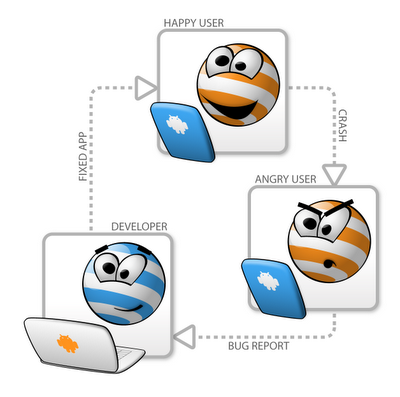
\includegraphics[width=10cm]{Imagenes/crash_report}
\caption{Concepto de Google sobre como el proceso de reportar crashes hacen al usuario feliz. \cite{18}}
\label{fig:Fig13}
\end{figure}

Este proceso es fundamental para el desarrollo y mantenimiento de una aplicaci�n, pues gracias a los reportes de crashes es posible saber en qu� casos es necesario realizar mejoras en el c�digo para dar m�s estabilidad a la aplicaci�n y que los errores pasados no se vuelvan a cometer. Como se puede ver en la figura \ref{fig:Fig13}, la idea b�sica es recibir feedback del usuario para reparar la aplicaci�n y que �ste tenga una mejor experiencia la pr�xima vez.


% ---------------------------------------------------------------------------------------------------------------
% Cap�tulo 3: Herramientas Actuales
% ---------------------------------------------------------------------------------------------------------------
\chapter{Herramientas Actuales}
\label{ch:herram}

En este cap�tulo se detallar�n las herramientas m�s utilizadas para combatir los diversos problemas durante el proceso de desarrollo de aplicaciones Android.



\section{Herramientas de Testing}
Ahora que ya se conoce lo b�sico sobre testing y se han visto las herramientas que entrega el framework de testing de Android, se comenzaran a ver el resto de herramientas que se encuentran disponibles. 

\subsection{Herramientas de testing provistas por Android}
Android provee un buen framework de testing \cite{20} para hacer pruebas en varios aspectos de la aplicaci�n. Los elementos claves son:
\begin{itemize}
\item Los Test suites (conjuntos de prueba) de Android est�n basados en JUnit. Se puede usar JUnit puro para testear una clase que no hace llamadas a la API de Android, o las extensiones de JUnit para Android si se desea testear componentes de Android. 

\item Las extensiones de JUnit proveen clases con tests espec�ficos para componentes. Estas clases entregan m�todos para crear \textit{mocking objects} (objetos simulados) y m�todos que ayudan a controlar el ciclo de vida de los componentes.

\item El SDK (Software Development Kit) de Android tambi�n provee herramientas para realizar testing a la UI, como \textit{monkeyrunner}.

\end{itemize}

A continuaci�n se revisar� en detalle cada una de las herramientas relacionadas a testing del SDK:

\subsubsection{JUnit}
El testing de Android se basa en JUnit. Actualmente la API de testing soporta JUnit 3. Este requiere que las clases de test hereden de la clase \textit{junit.framework.TestCase}. Adem�s, en JUnit 3 los m�todos de testing deben comenzar con el prefijo \textit{test}. Tambi�n se debe llamar al m�todo \textit{setUp()} para configurar el test y al m�todo \textit{tearDown()} para finalizar el test.\\

Es una buena pr�ctica, al realizar testing en Android, tener un m�todo llamado \textit{testPreconditions()} que se encargue de corroborar las precondiciones para cada uno de los test. Si este m�todo falla, se sabe inmediatamente que las suposiciones para los otros test no se han cumplido.\\

Se puede usar la clase \textit{TestCase} de JUnit para hacer testing unitario en una clase que no haga llamadas a la API de Android. \textit{TestCase} es tambi�n la clase base para \textit{AndroidTestCase}, que puede ser usada para testear objetos que dependen de Android.\\

La clase \textit{Assert} de JUnit es usada para mostrar los resultados de los test. Los m�todos \textit{assert} comparan los valores que se esperan de un test con los valores reales y se lanza una excepci�n si la comparaci�n falla. Android tambi�n provee una clase para \textit{assertions} que extiende los posibles tipos de comparaciones, y otra clase de \textit{assertions} para testear la UI.

\subsubsection{Instrumentation}
La API de testing de Android provee interacciones entre los componentes de Android y el ciclo de vida de la aplicaci�n. Estas interacciones son realizadas a trav�s de la API Instrumentation, que permite a los tests controlar el ciclo de vida y los eventos de interacci�n del usuario.\\

Normalmente, un componente de Android se ejecuta en un ciclo de vida determinado por el sistema. Por ejemplo, el ciclo de vida de un objeto \textit{Activity} comienza cuando este es activado por un \textit{Intent}. El m�todo \textit{onCreate()} es llamado, seguido del m�todo \textit{onResume()}. Cuando el usuario abre otra aplicaci�n, el m�todo \textit{onPause()} es llamado. Si la Actividad llama al m�todo \textit{finish()}, entonces el m�todo \textit{onDestroy()} tambi�n es llamado. La API de Android no provee un forma de llamar estos m�todos directamente, pero se puede hacer a trav�s de \textit{Instrumentation}.\\

�nicamente una clase de test basada en \textit{Instrumentation} permite enviar eventos de teclado o toques de pantalla a la aplicaci�n bajo test. Por ejemplo, se puede testear una llamada al m�todo \textit{getActivity()}, el cu�l comienza una actividad y retorna la actividad que est� siendo testeada. Despu�s se puede llamar al m�todo \textit{finish()}, seguido por un m�todo \textit{getActivity()} nuevamente, y as� poder testear si la aplicaci�n restaura su estado de forma correcta.\\

El sistema ejecuta todos los componentes de una aplicaci�n en el mismo proceso. Se puede permitir a algunos componentes, tales como \textit{Content Providers}, ejecutarse en un proceso separado, pero no se puede forzar a una aplicaci�n a ejecutarse en el mismo proceso en el que otra aplciaci�n esta ejecut�ndose.\\

\subsubsection{Simulando objetos (Mock objects)}
Android entrega clases para crear objetos llamados \textit{mock objects}, que son objetos de sistema simulados como Context, ContentProvider, ContentResolver y Service. Algunos tests tambi�n proveen objetos simulados de Intent. Se pueden usar estos \textit{mocks} para aislar los tests del resto del sistema y facilitar la inyecci�n de dependencias. Estas clases se encuentran en los paquetes \textit{android.test} y \textit{android.test.mock}.\\

Por ejemplo se puede usar MockContext en vez de Context. La clase \textit{RenamingDelegatingContext} entrega las llamadas a un contexto dado y ayuda a la base de datos y a las operaciones con archivos agregando un prefijo a todos los nombres de los archivos. De esta forma se pueden testear compontentes sin afectar la base de datos del sistema de archivos de un dispositivo Android.

\subsubsection{uiautomator}
El SDK de Android contiene la biblioteca \textit{uiautomator} para testear y ejecutar tests a la interfaz gr�fica. Esto fue implementado a partir de la API 16 \cite{19}.

Los proyectos de test de \textit{uiautomator} son proyectos en Java, en donde la biblioteca de JUnit 3, junto con los archivos uiautomator.jar y android.jar son agregados a la compilaci�n. 

Adem�s esta biblioteca provee la clase UiDevice que permite la comunicaci�n con el dispositivo, la clase UiSelector para buscar elementos en la pantalla y la clase UiObject que presenta los elementos de la interfaz. La clase UiCollection permite seleccionar un n�mero de elementos de la interfaz gr�fica al igual que la clase UiScrollable permite hacer scroll en una vista apra encontrar un elemento.

\subsubsection{uiautomatorviewer}
Android tambi�n provee la herramienta \textit{uiautomatorviewer}, que permite analizar la interfaz gr�fica de una aplicaci�n. Esta herramienta puede ser usada apra encontrar los id, texto o atributos de los elementos de la interfaz.

Esta herramienta permite a la gente que no programa, analizar una aplicaci�n y desarrollar test a trav�s de la biblioteca \textit{uiautomator}. 
[AGREGAR SCREENSHOT]

\subsubsection{Monkey}
\textit{Monkey} \cite{21}  es un herramienta de l�nea de comando que envia eventos aleatorios a un dispositivo. Se puede restringir a \textit{Monkey} para que se ejecute �nicamente en ciertos paquetes, por lo que se le pueden dar instrucciones para testear �nicamente una aplicaci�n.

Por ejemplo, el siguiente comando enviar� 2000 eventos aleatorios a la aplicaci�n con el nombre de paquete co.seahorse.android:\\

\begin{lstlisting}
adb shell monkey -p co.seahorse.android -v 2000
\end{lstlisting}

\subsubsection{monkeyrunner}
La herramienta monkeyrunner provee una API en Python para escribir programas que controlen un dispositivo Android o un emulador, fuera del c�digo fuente que hayamos escrito.

A trav�s de \textit{monkeyrunner} se puede hacer un script para realizar un test. Este se ejecuta atrav�s del adb debug bridge y permite instalar programas, iniciarlos, controlar los flujos y tomar screenshots.

Para usar \textit{monkeyrunner} se debe tener instalado Python en el computador.

Las siguientes clases son las principales:
\begin{itemize}
\item MonkeyRunner: permite conectarse con los dispositivos.

\item MonkeyDevice: permite instalar y desintalar aplicaciones, como tambi�n enviar eventos de teclado y toques en la pantalla a una aplicaci�n.

\item MonkeyImage: Permite crear, comparar y guardar screenshots.
\end{itemize}

\subsection{Herramientas de testing de terceros}
\subsubsection{EasyMock}
EasyMock es un framework para mocking \cite{22}, es decir, para crear objeto simulados. Este puede ser usado en conjunto con JUnit. A continuaci�n se muestra como es la instanciaci�n de un objeto basado en una clase.\\

\begin{lstlisting}
import static org.easymock.EasyMock.createNiceMock;
....

// ICalcMethod es el objeto que es simulado
ICalcMethod calcMethod = createNiceMock(ICalcMethod.class); 
\end{lstlisting}

El m�todo createNiceMock() crea un mock que retorna los valores por defecto para m�todos que no est�n sobreescritos. Adem�s tiene varios m�todos que pueden ser usados para configurar el objeto mock. El m�todo expect() le dice a Easymock que simule un m�todo con ciertos argumentos. El m�todo andReturn() define lo que va a retornar este m�todo. El m�todo times() define que tan seguido el objeto va a ser llamado.


\subsubsection{Mockito}
Mockito \cite{23} es un framework bastante popular que puede ser usado en conjunto con JUnit. Este permite crear y configurar objetos simulados. Adem�s, desde la versi�n 1.9.5 puede ser usado directamente con los test de Android.

Mockito soporta la creaci�n de objetos simulados con el m�todo est�tico \textit{mock()}. Este tambi�n soporta la creaci�n de objetos basados en la anotaci�n \textit{@Mock}. Si se usan anotaciones, se debe inicializar el objeto similado con una llamada al m�todo \textit{MockitoAnnotations.initMocks(this)}.


\subsubsection{Robolectric}
Robolectric \cite{24} es un framework que simula parte del framework de Android contenido en el archivo \textit{android.jar}. Esta dise�ado para permitir testear aplicaciones de Android en la JVM (Java Virtual Machine). Este permite ejecutar los test de Android en un entorno de integraci�n continua, sin necesidad de configuraciones extras. Est� basado en JUnit 4.

Robolectric reemplaza todas las clases de Android por los llamados shadow objects. Si un m�todo es implementado por Robolectric, este dirige estas llamadas al shadow object, que se comporta de forma similar a los objetos del SDK de Android. Si un m�todo no es implementado por el shadow object, este simplemente retorna un valor por defecto, como null o 0.

Robolectric soporta el manejo de recursos, como inflar vistas. Tambi�n puede usarse el findViewById() para buscar una vista.

\subsubsection{Robotium}
Robotium \cite{25} es una extensi�n del framework de test de android y fue creado para hacer m�s f�cil los test de interfaz gr�fica para las aplicaciones de Android. Robotium hereda de ActivityInstrumentationTestCase2 y permite definir casos de test a trav�s de las actividades de Android.

Los test con Robotium interactuan con la aplicaci�n como test de caja negra, esto quiere decir que �nicamente se interactua con la interfaz y no a trav�s del c�digo interno de la aplicaci�n. La clase principal para testear con Robotium se llama Solo. Esta es inicializada en la primera actividad que se desea testear.

\subsubsection{Espresso}
Google lanz� el framework Espresso \cite{26} para testing en Octubre del 2013.  Esta es una API para realizar tests de interfaz gr�fica, localizando elementos de la UI e interactuando con ellos. A continuaci�n se presentan los componentes principales de Espresso:\\

\begin{itemize}
\item Espresso: Punto de entrada para interactuar con las vistas, a trav�s de los m�todos \textit{onView()} y \textit{onData()}. Tambi�n permite la interacci�n con m�todos que no necesariamente estan atados a una vista, como por ejemplo el m�todo \textit{pressBack()}.

\item ViewMatchers: Una colecci�n de objetos que implementan la interfaz \textit{Matcher<? super View>}. Se puede pasar uno o m�s de estos objetos al m�todo \textit{onView()} para localizar una vista que actualmente este dentro de la jerarqu�a de vistas.

\item ViewActions: Una colecci�n de \textit{ViewActions} que pueden pasarse al m�todo \textit{ViewInteraction.perform}, por ejemplo un click.

\item ViewAssertions: Una colecci�n de ViewAssertions que pueden pasarse al m�todo  \textit{ViewInteraction.perform}. 
\end{itemize}


\subsubsection{Spoon}
Spoon es una herramienta de c�digo abierto para test automatizados que permite ejecutar los test escritos en java en varios dispositivos al mismo tiempo. Este fue desarrollado por la compa��a Square \cite{27}.

La aplicaci�n se ejecuta en base a los test que hayamos definido en las pruebas de instrumentaci�n. Spoon genera un informe con los resultados a trav�s de un HTML. Cada dispositivo testeado tiene una ficha con los resultados de cada uno de los test.

Adem�s, Spoon permite obtener screenshot de cada estado que se haya definido en la ejecuci�n de los test, los cuales pueden verse en las distintas resoluciones de cada dispositivo en los que se realizaron las pruebas. En el siguiente c�digo se obtienen dos screenshots, uno al inicio y otro despu�s de realizar los respectivos test:

\begin{lstlisting}
Spoon.screenshot(activity, "initial_state");
/* aqui va un codigo de test... */
Spoon.screenshot(activity, "after_login");
\end{lstlisting}

\subsubsection{Remote Test Lab}
Remote Test Lab \cite{28} es un servicio que Samsung ofrece a los desarrolladores para que puedan probar sus aplicaciones en un dispositivo real, pero en remoto. Gracias a �l podr�n acceder, v�a web, a diferentes smartphones y tablets con varias versiones del sistema operativo. En estos dispositivos los desarrolladores podr�n instalar y testear sus apps...

\section{Herramientas de reporte de crashes}
Una vez publicada una aplicaci�n, comienza el proceso de correcciones de errores y mejoras. Esto se puede realizar gracias a los reportes de crashes que se reciben cuando la aplicaci�n deja de funcionar correctamente. Es muy importante corregir todos estos errores para dar mayor estabilidad a la aplicaci�n y para ofrecer un mejor producto al usuario. Android cuenta con un sistema de reporte de crashes desde el a�o 2010\cite{18}. A continuaci�n se revisar�n las caracter�sticas con las que cuenta:

\subsection{Herramienta de reporte de crashes provista por Android}
Cuando la aplicaci�n ya esta publicada, es posible acceder a una secci�n dentro de la \textit{Google Play Developer Console} \cite{29}, titulada \textit{CRASHES \& ANRS}. En este sitio es posible ver los reportes de los �ltimos 6 meses. Tal como se muestra en la figura \ref{fig:Fig14}, es posible aplicar distintos filtros para obtener informaci�n m�s detallada sobre estos reportes. Por ejemplo, se puede filtrar por versiones de sistema operativo o el n�mero de versi�n de la aplicaci�n.

\begin{figure}[h!]
\centering
      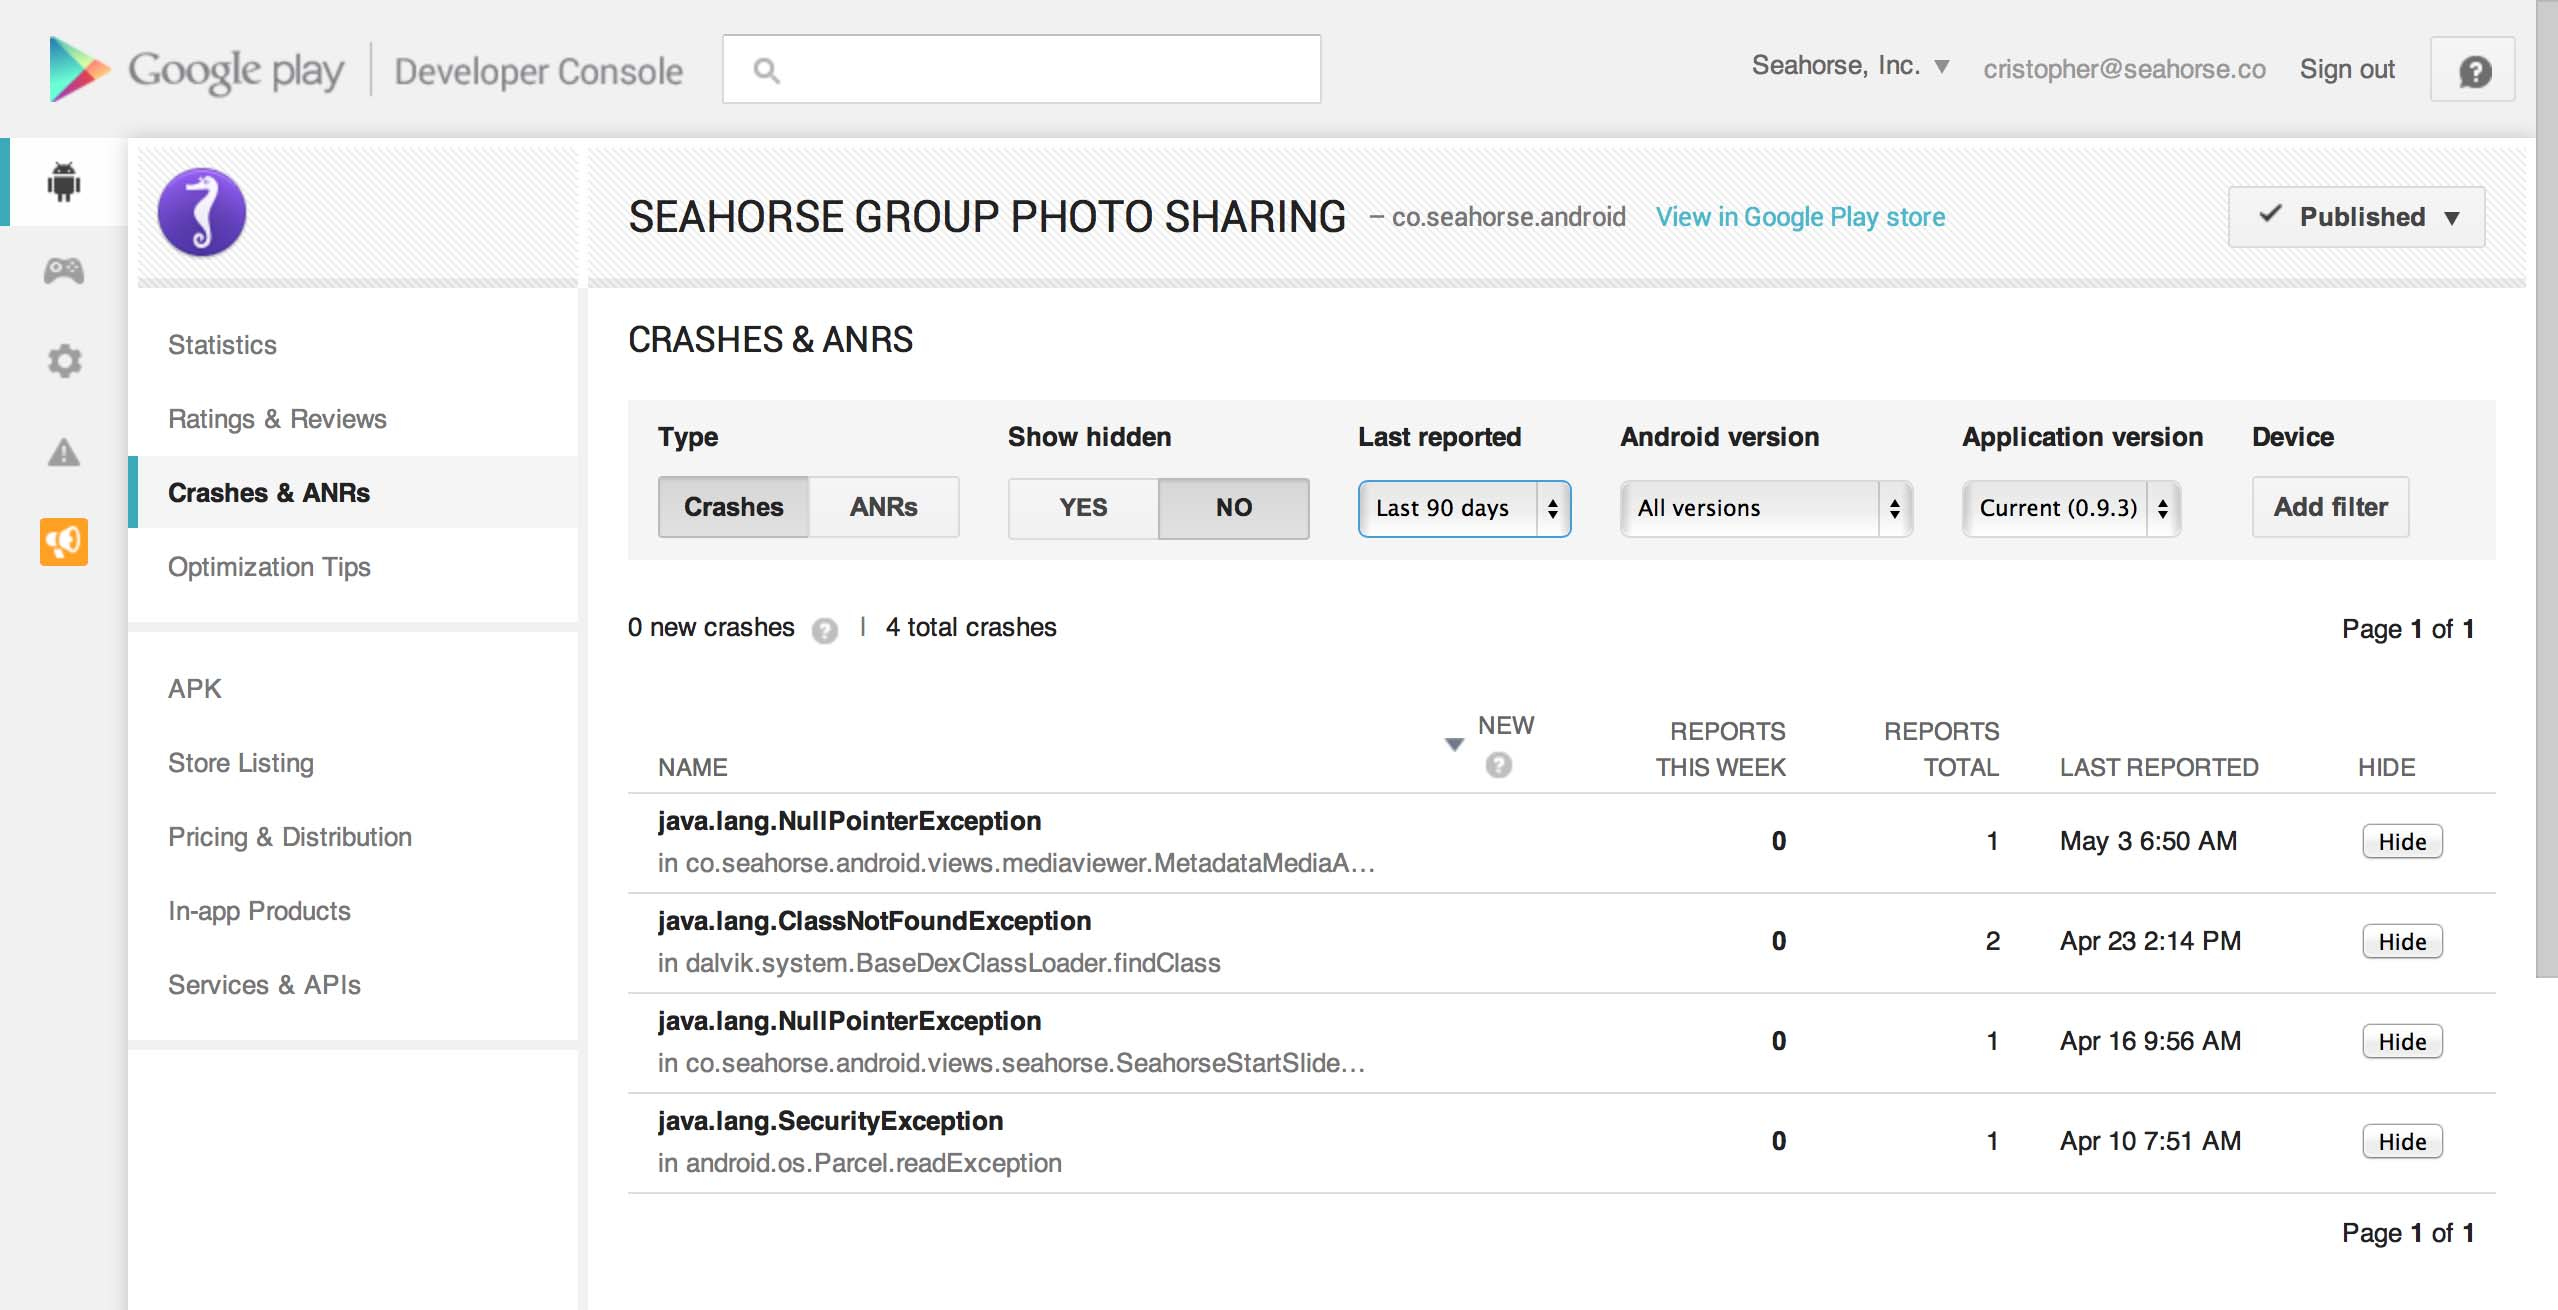
\includegraphics[width=15cm]{Imagenes/crash_report_google}
\caption{Vista del sistema de reporte de crashes provisto por Android.}
\label{fig:Fig14}
\end{figure}

Tal como se mencion� anteriormente, estos reportes son los que env�a el usuario cuando la aplicaci�n deja de funcionar correctamente. En ese momento, el sistema le pregunta al usuario si desea enviar el reporte del crash al desarrollador. Adem�s, el usuario tiene la opci�n de enviar alg�n mensaje adicional que pueda ser �til para el desarrollador, como por ejemplo, que al momento del crash se estaba usando la c�mara. 

Al presionar en el reporte de crash para ver m�s detalles, se puede ver la hora y el d�a en el que ocurri� el crash, cuantas veces ha ocurrido y el dispositivo que estaba usando el usuario. Tambi�n se pueden ver algunas l�neas del stack trace del usuario al momento del error. El stack trace es un reporte de todas las acciones que se realizan en cierto punto, durante la ejecuci�n de una aplicaci�n. Esto es muy �til para los desarrolladores ya que la mayor�a de las veces se puede ver en que l�nea del c�digo la aplicaci�n dej� de responder correctamente y que tipo de error ocurri�. Con esta informaci�n es posible comenzar a revisar el c�digo y ver que problema existe.

\subsection{Herramientas de reporte de crashes de terceros}
Existen varias herramientas que entregan reportes de crashes mucho m�s completos que los que entrega Google de forma nativa. La mayor�a de estas entregan una versi�n gratuita con restricciones y es posible pagar para acceder a la versi�n premium, la cual cuenta con caracter�sticas m�s especializadas. Adem�s, todos los reportes de crashes son env�ados, ya que al momento de instalar la aplicaci�n se piden los permisos necesarios para ello, por lo que el usuario afectado no debe hacer nada. A continuaci�n se listan las m�s populares: 
\subsection{Crittercism}
Crittercism es un sistema muy completo que cuenta con monitoreo, manejo de excepciones, como tambi�n reportes de crashes y performance. Actualmente soporta m�ltiples plataformas, entre las que se encuentran: Android, Android NDK, iOS, Windows Phone 8 y HTML5.  

La instalaci�n es bastante simple \cite{31}. Se debe descargar el SDK de Crittercism para Android e incluirlo al proyecto. Luego se deben agregar los siguientes permisos en el archivo Android Manifest del proyecto: 
\begin{lstlisting}
<uses-permission android:name="android.permission.INTERNET"/>
<uses-permission android:name="android.permission.READ_LOGS"/>
<uses-permission android:name="android.permission.ACCESS_NETWORK_STATE"/>
<uses-permission android:name="android.permission.GET_TASKS"/>
\end{lstlisting}
El primer permiso es necesario para poder acceder a Internet y poder enviar los reportes. El segundo es necesario para poder obtener la informaci�n de los stack trace del usuario, y ahi saber en que l�nea de c�digo ha ocurrido el error. El tercero es para obtener informaci�n sobre el estado de la red, por ejemplo, para saber si el usuario est� conectado a Wi-Fi o a trav�s de un carrier. El �ltimo permiso sirve para acceder a la informaci�n de las �ltimas dos actividades ejecutadas, lo que permite saber en que actividad ocurri� el crash.

Una vez que los permisos ya est�n entregados, se debe inicializar Crittercism. Esto se hace �nicamente una vez por aplicaci�n, por lo que se debe hacer en la primera actividad que se ejecuta dentro de la aplicaci�n. Para iniciar Crittercism se escribe la siguiente l�nea en el onCreate:
\begin{lstlisting}
Crittercism.initialize(getApplicationContext(), "CRITTERCISM_APP_ID");
\end{lstlisting}

Ahora ya est�n implementadas las caracter�sticas b�sicas, y comenzar�n a llegar los reportes al sitio de Crittercism. Tambi�n es posible recibir cada reporte de crash al correo, configurando esto desde el sitio web.

Como se puede ver en la figura \ref{fig:Fig15}, se tienen opciones parecidas al reporte de crashes de Google. La gran diferencia est� en el detalle de la informaci�n, ya que al revisar los detalles de un crash, se puede ver informaci�n muy espec�fica como: nivel de bateria, espacio en el disco, espacio en la tarjeta SD, uso de RAM, estabilidad de la red, orientaci�n del dispositivo, idioma del dispositivo, actividades que estaban ejecutandose, entre muchos otros puntos.
\begin{figure}[h!]
\centering
      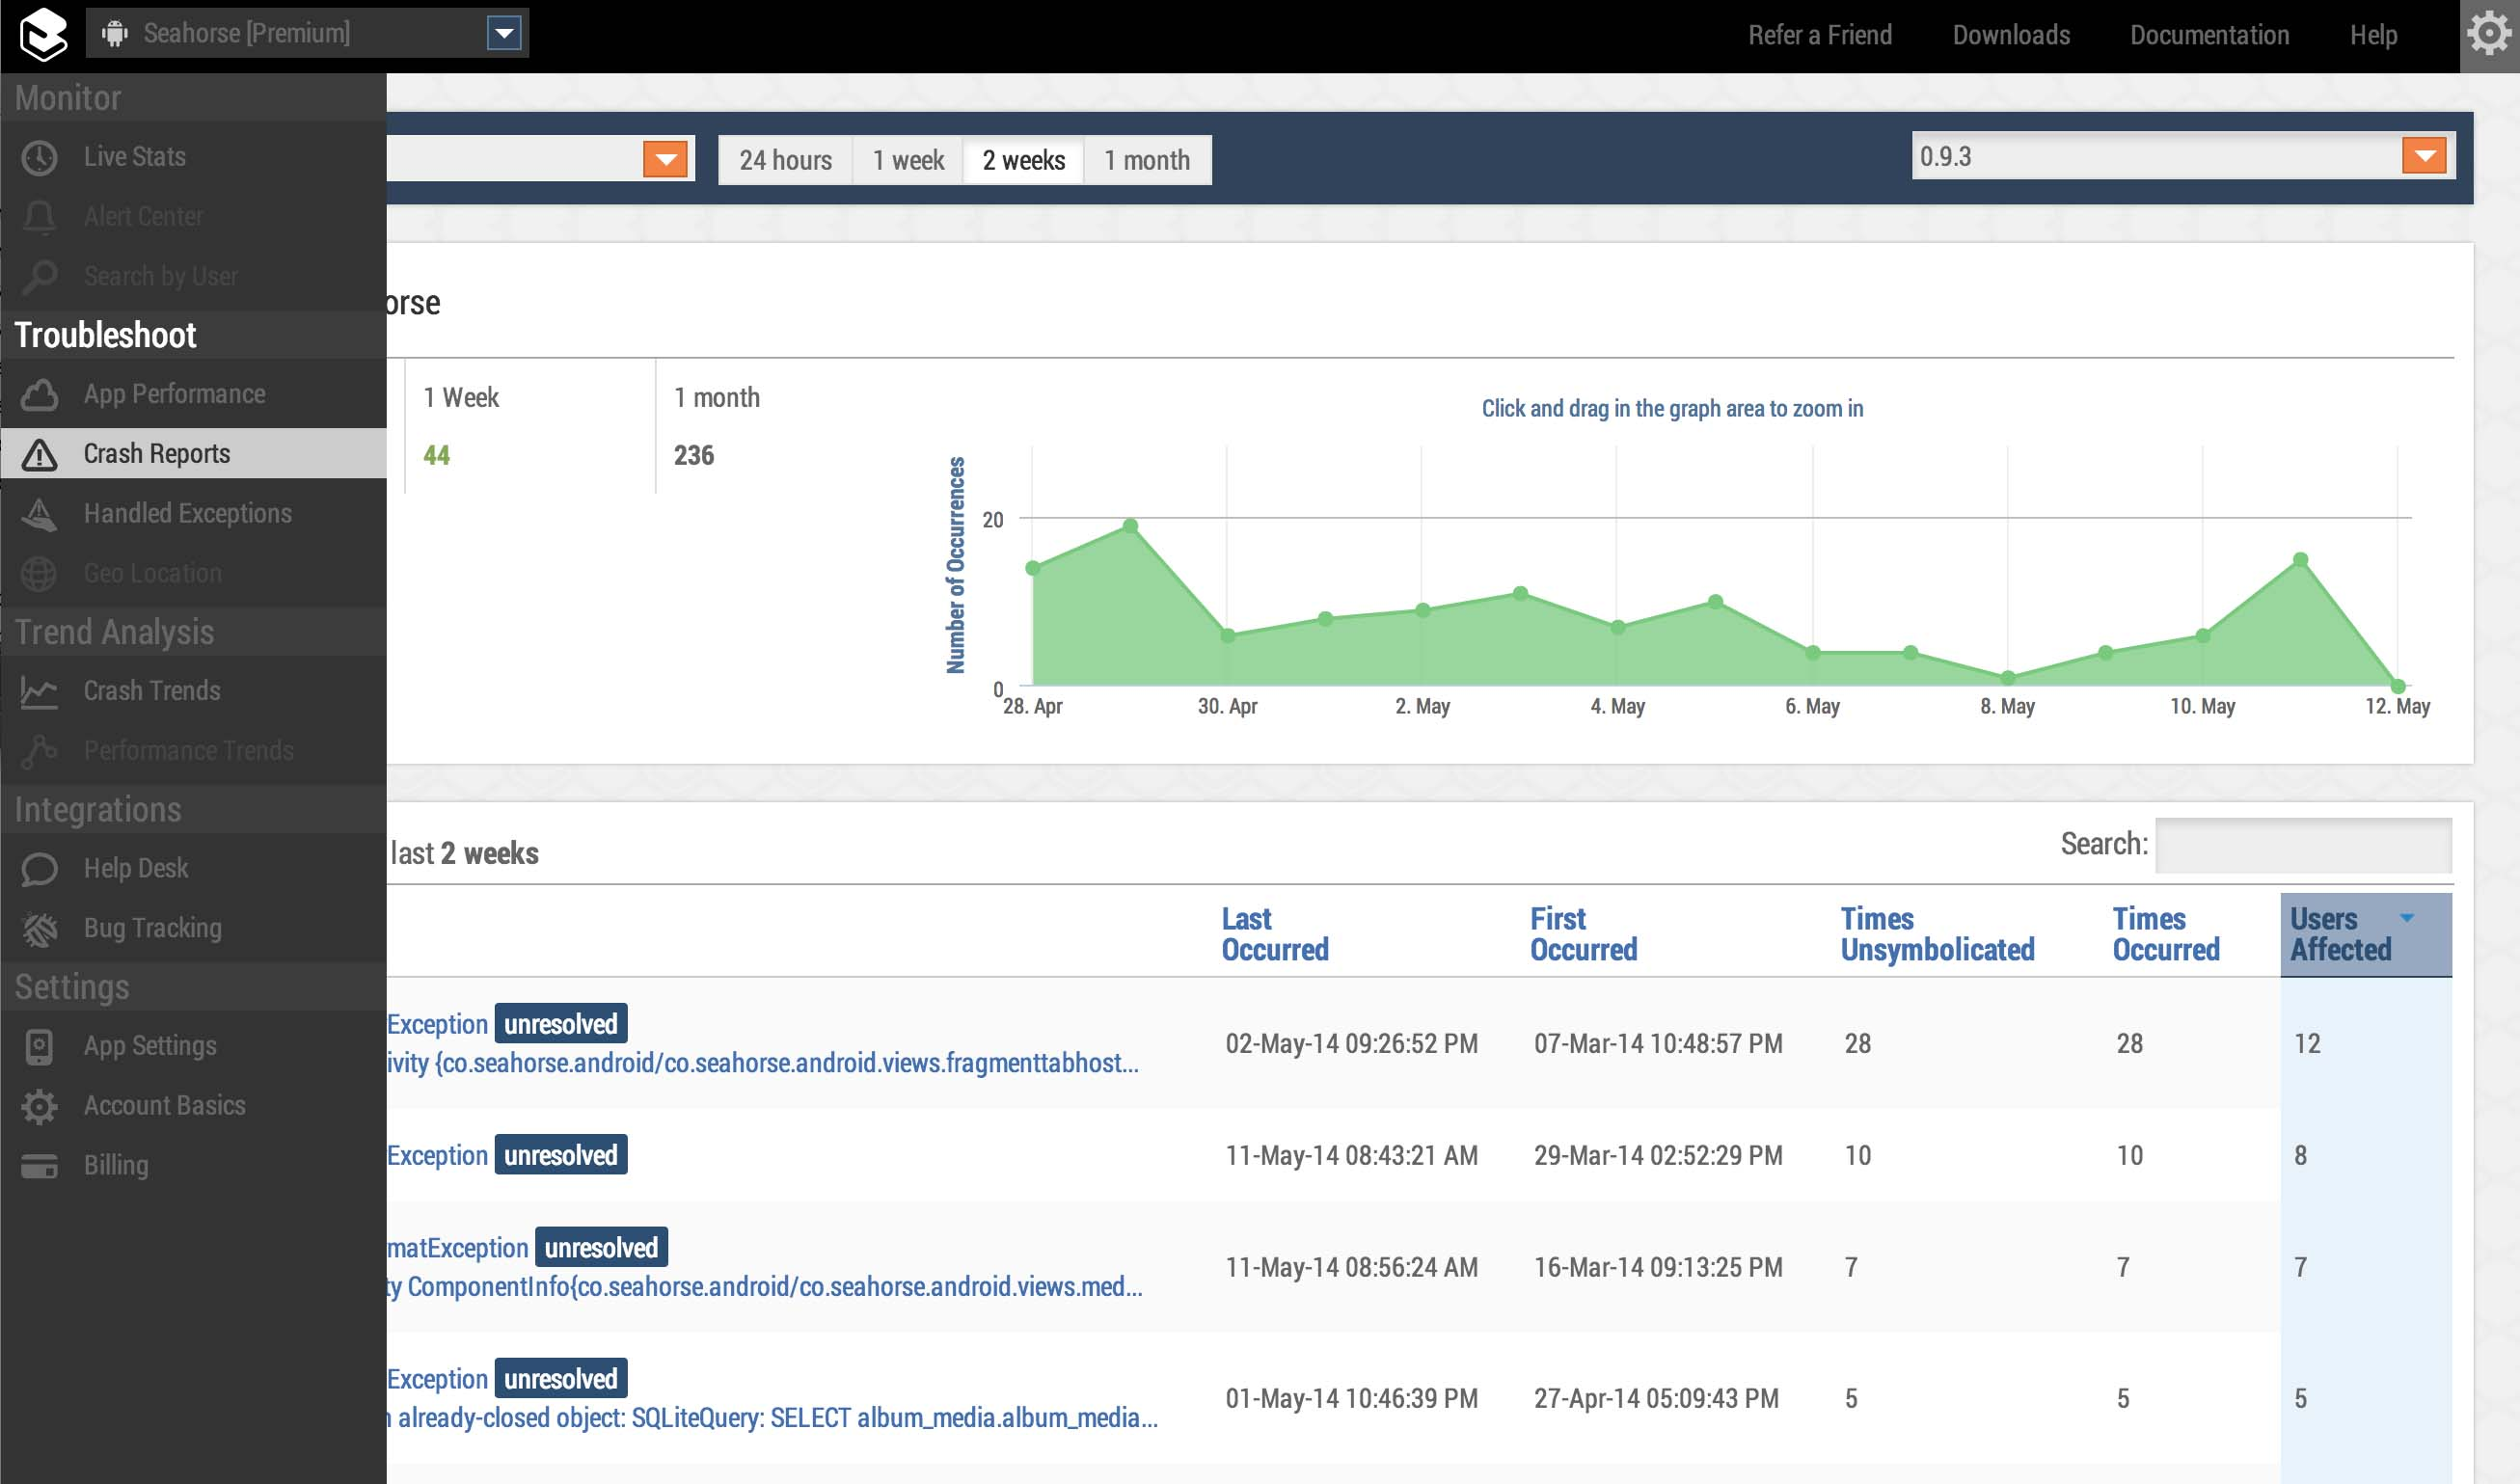
\includegraphics[width=15cm]{Imagenes/crash_report_crittercism}
\caption{Vista del sistema de reporte de crashes de Crittercism}
\label{fig:Fig15}
\end{figure}

\subsection{Bugsense}
Bugsense tambi�n es un sistema bastante completo. Cuenta con monitoreo, reportes de crashes, manejo de excepciones, tendencias de crashes e integraci�n con ACRA. Soporta m�ltiples plataformas, entre las que se encuentran: Android, iOS, Windows Phone 8 y HTML5.  

Para la instalaci�n se descarga la biblioteca desde el sitio de Bugsense \cite{32}. Despu�s de incluirla en el proyecto, se deben pedir los permisos correspondientes en el Android Manifest. Para iniciar Bugsense se escribe la siguiente l�nea:   
\begin{lstlisting}
BugSenseHandler.initAndStartSession(Context, APIKEY);
\end{lstlisting}


Con esto, Bugsense ya se encuentra implementado. Para implementar las otras caracter�sticas s�lo hay que seguir el tutorial que se encuentra en el sitio\cite{32}. 

En la figura \ref{fig:Fig16} se puede ver como es el panel con estad�sticas que ofrece Bugsense. Similar a lo ofrecido por Crittercism, es posible filtrar los crashes por versi�n de la aplicaci�n, como tambi�n por versi�n del sistema operativo.

\begin{figure}[h!]
\centering
      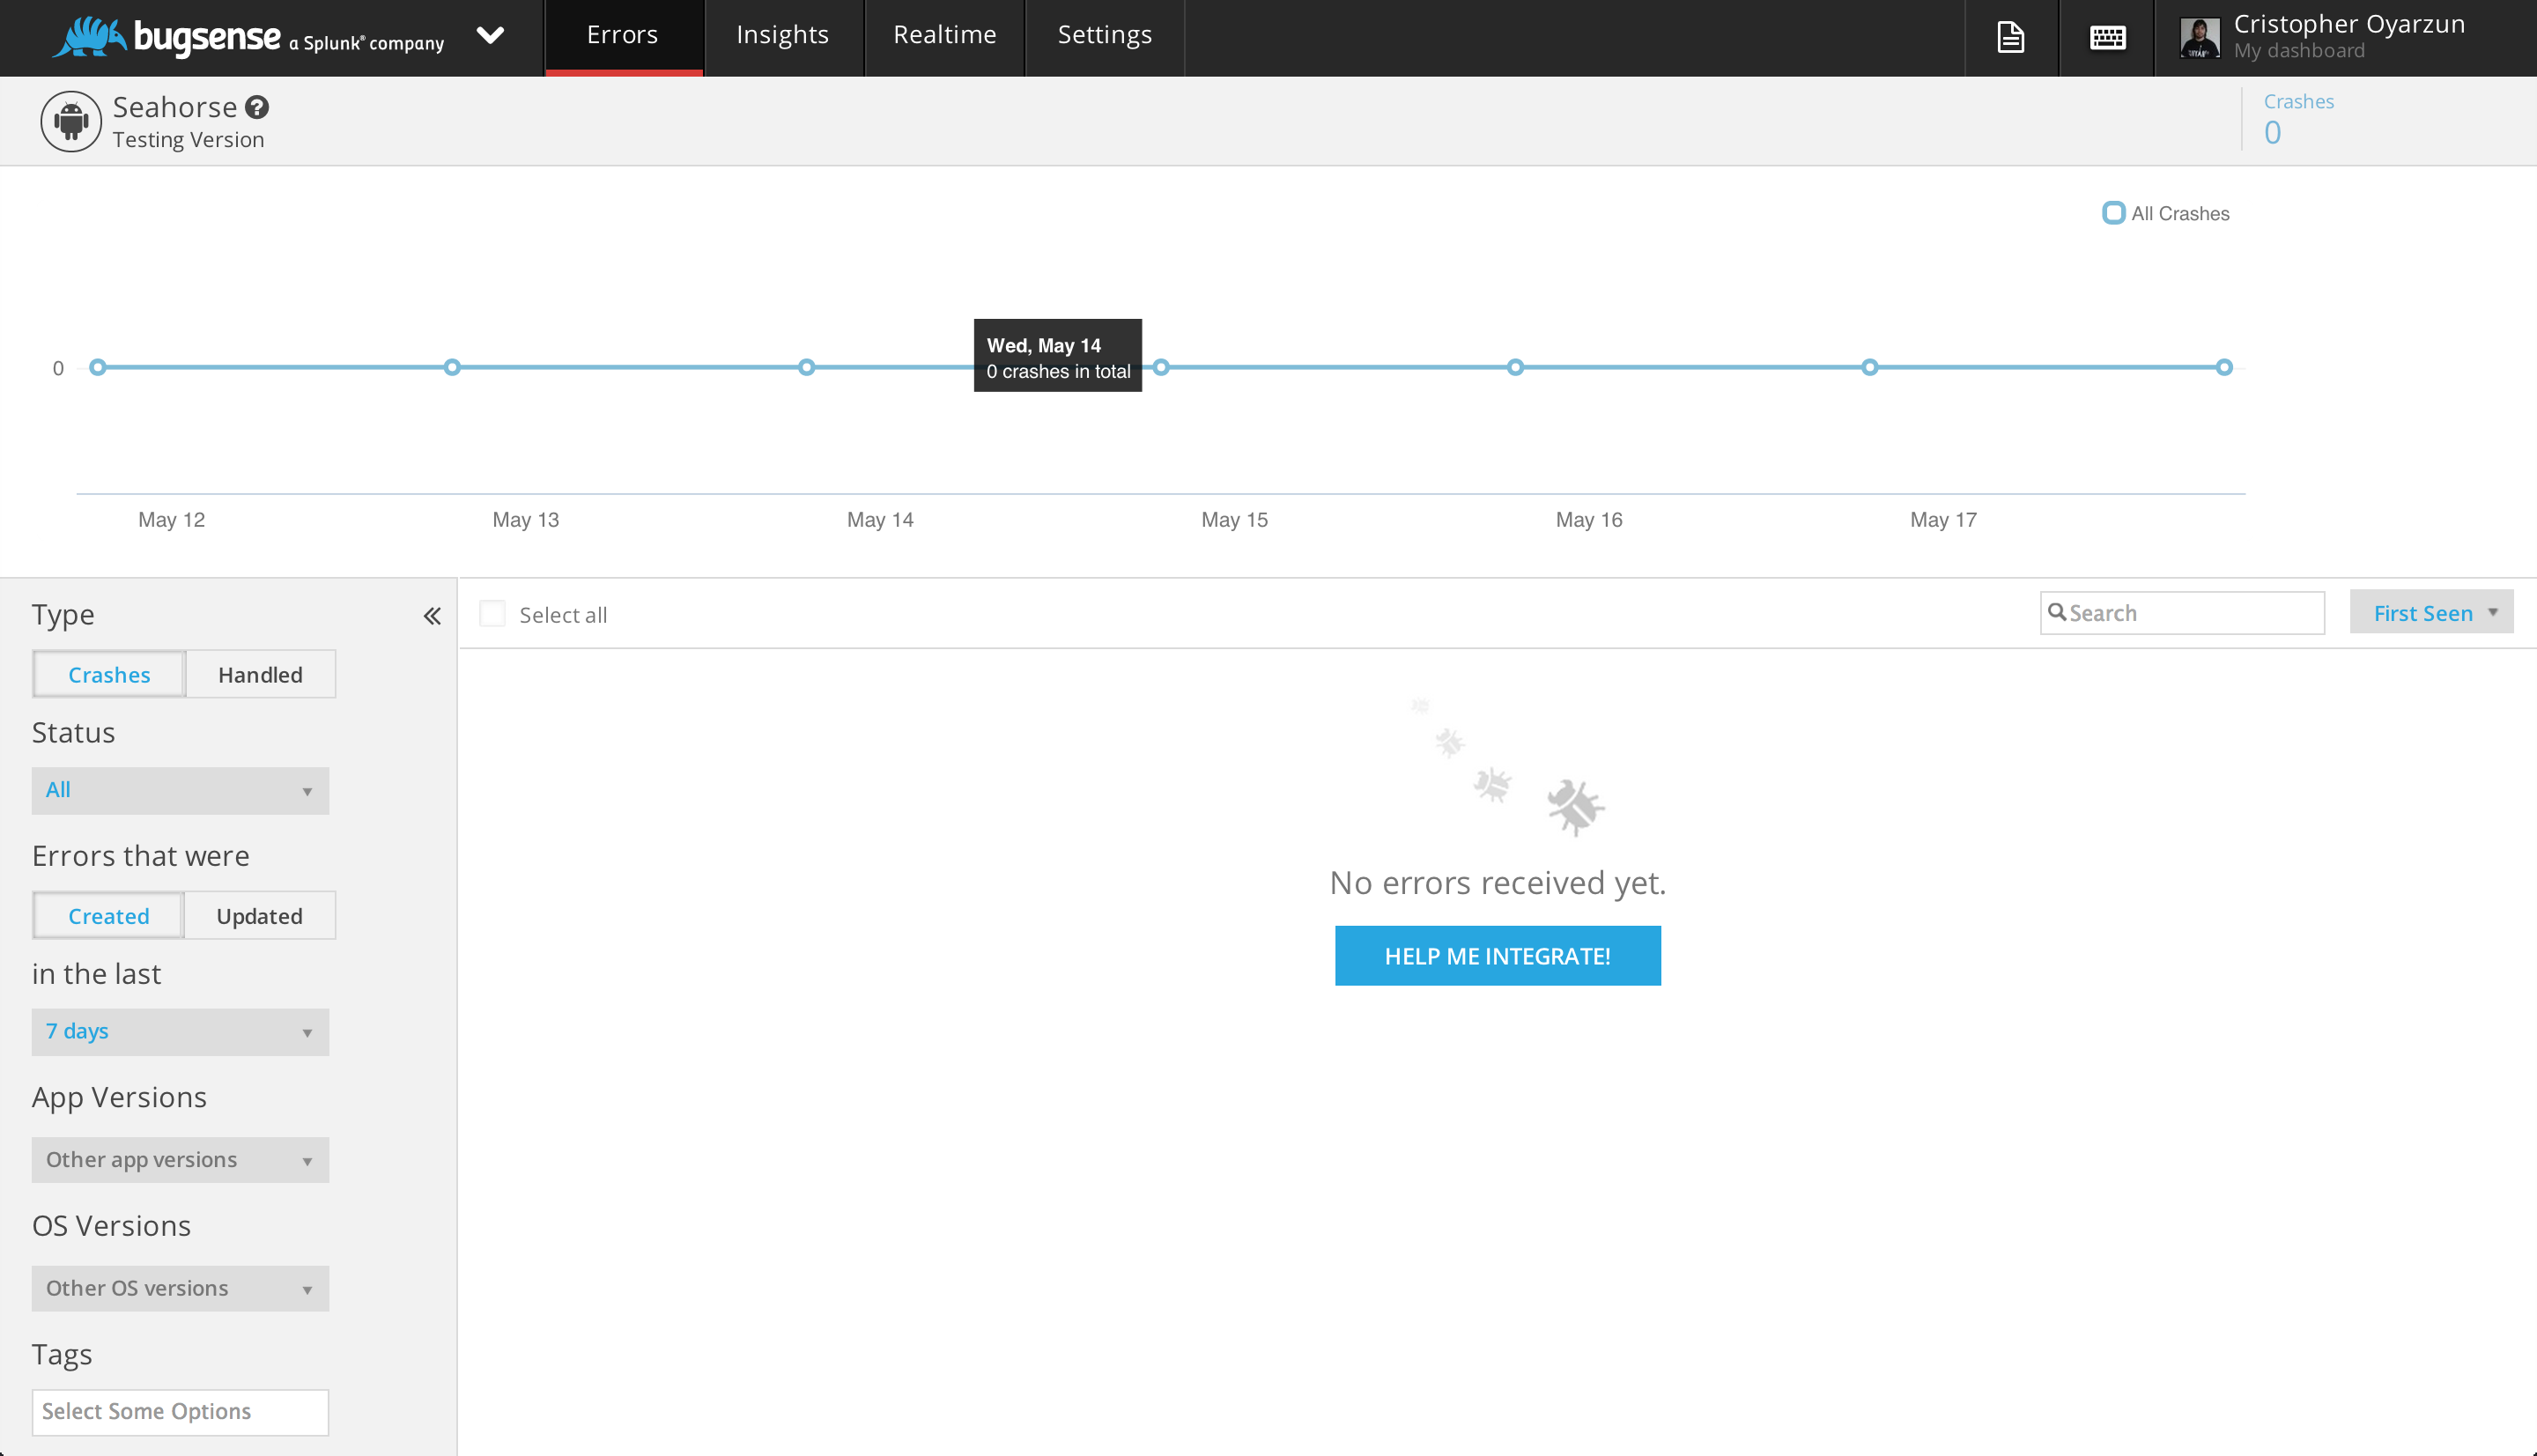
\includegraphics[width=15cm]{Imagenes/crash_report_bugsense}
\caption{Vista del sistema de reporte de crashes de Bugsense}
\label{fig:Fig16}
\end{figure}

\subsection{Google Analytics}
Google Analytics es otra herramienta que cuenta con reportes de crashes. Si bien, la especialidad de Google Analytics es ofrecer estad�sticas y hacer tracking de distintos eventos, tambi�n es posible recibir reportes de crashes y excepciones. El gran problema es que los reportes no llegan en tiempo real, ya que la informaci�n se actualiza con un d�a de retraso.

Para su implementaci�n es necesario descarga desde el sitio de Google Analytics \cite{33} la versi�n 3 de su SDK. Una vez descargado el SDK, es necesario incluirlo al proyecto y dar los siguientes permisos en el archivo Android Manifest:
\begin{lstlisting}
<uses-permission android:name="android.permission.INTERNET"/>
<uses-permission android:name="android.permission.ACCESS_NETWORK_STATE"/>
\end{lstlisting}
Para implementarlo a trav�s de c�digo es necesario agregar estas l�neas en cada una de las Actividades de las cu�les se desee obtener informaci�n:
\begin{lstlisting}
@Override
  public void onStart() {
    super.onStart();
    ... // El resto del c�digo de onStart()
    EasyTracker.getInstance(this).activityStart(this);  // Agregar este m�todo
  }

  @Override
  public void onStop() {
    super.onStop();
    ... // El resto del c�digo de onStop()
    EasyTracker.getInstance(this).activityStop(this);  // Agregar este m�todo
  }
\end{lstlisting}
Google Analytics ofrece filtrar los reportes de crashes por versi�n de la aplicaci�n, versi�n del sistema operativo, marca del dispositivo y tama�os de pantalla.

\subsection{ACRA}
ACRA es una biblioteca gratuita y de c�digo abierto disponible en Github \cite{35}. Desde la �ltima actualizaci�n de Google Forms, el uso de Google Docs como almacenamiento para los reportes que entregaba ACRA est� obsoleto. Ahora es necesario implementar una aplicaci�n web para poder ver los reportes, aunque tambi�n es posible asociarlo a otras plataformas como Bugsense o HockeyApp. 

Para su implementaci�n es necesario descarga la biblioteca desde el sitio web de ACRA \cite{34}. Una vez que ya se ha a�adido al proyecto, es necesario pedir el siguiente permiso en el archivo de Android Manifest:
\begin{lstlisting}
<uses-permission android:name="android.permission.INTERNET"/>
\end{lstlisting}
En el c�digo del proyecto la implementaci�n es de la siguiente forma:
\begin{lstlisting}
import org.acra.*;
import org.acra.annotation.*;

@ReportsCrashes(formKey = "", formUri = "http://www.aqui_va_la_plataforma_web.com/reportpath")
public class MyApplication extends Application {
  @Override
  public void onCreate() {   
    super.onCreate();
    ACRA.init(this);  // Esta es la l�nea que inicializa ACRA
  }
}			
\end{lstlisting}





% ---------------------------------------------------------------------------------------------------------------
% Cap�tulo 4: An�lisis Comparativo
% ---------------------------------------------------------------------------------------------------------------
\chapter{An�lisis Comparativo}
\label{ch:analis}
Para llevar a cabo estos an�lisis comparativos, en algunos casos las herramientas se han subdividido en m�s categorias. De esta forma es posible realizar comparaciones que arrojen resultados m�s relevantes y �tiles. Las ventajas y desventajas de cada herramienta ayudar�n a determinar cu�l se ajusta m�s a las necesidades del desarrollador.

En cada secci�n se agregar� un resumen general, el cu�l incluir� una tabla comparativa y conclusiones que actuar�n como gu�a para los desarrolladores.

En el siguiente cap�tulo se llevar� a cabo la implementaci�n de las herramientas m�s destacadas en una aplicaci�n que se encuentra disponible en la tienda oficial de Google.

\section{An�lisis Comparativo entre las Herramientas de Testing Unitario}
\subsection{Framework de Testing de Android}
\subsubsection{Ventajas}
\begin{itemize}
\item Acceso al Framework de Android.

\end{itemize}
\subsubsection{Desventajas}
\begin{itemize}
\item Los test son lentos ya que se ejecuten en un dispositivo real o un emulador con la m�quina virtual Dalvik.

\item Usa JUnit 3, en vez del m�s reciente JUnit 4.

\end{itemize}

\subsubsection{Resumen}
El Framework de testing de Android es el m�todo oficial que ofrece Google para realizar testing unitario. Primero se carga la aplicaci�n en un dispositivo, y luego los tests basados en JUnit se ejecutan. Debido a que se ejecutan en un dispositivo que cuenta con el sistema operativo Android, se pueden usar todos los m�todos que ofrece el framework de Android, por lo que los test son lo m�s cercano a la realidad. Aunque esto tambi�n le juega en contra, ya que compilar la aplicaci�n, subir la aplicaci�n a un dispositivo o emulador, y luego ejecutar los test es un proceso muy lento.

\subsection{Robolectric}
\subsubsection{Ventajas}
\begin{itemize}
\item Gratuito y de c�digo abierto.

\item Los test son r�pidos ya que se ejecutan en la m�quina virtual de Java, por lo que no se necesita tener un dispositivo conectado.

\item Comunidad que realiza mejoras de forma activa, con m�s de 4 a�os de desarrollo.

\end{itemize}
\subsubsection{Desventajas}
\begin{itemize}
\item Existe documentaci�n, pero falta actualizarla.

\item No todo puede realizarse con los \textit{mocks} ofrecidos en Robolectric.

\end{itemize}

\subsubsection{Resumen}
Robolectric es un proyecto de c�digo abierto que unifica la velocidad del testing unitario con la posibilidad de acceder el framework de Android. Esto se hace implementando todos los \textit{stubs} con \textit{mocks} clases. Es extremadamente r�pido en comparaci�n con lo que ofrece Android de forma nativa, ya que los test se ejecutan en una m�quina virtual de Java, no siendo necesario compilar todo el proyecto y cargar la aplicaci�n en un dispositivo. Sin embargo, debido al r�pido y constante desarrollo que ha tenido Robolectric, en las �ltimas versiones ha cambiado bastante, dejando obsoleta mucha de la documentaci�n existente.

\subsection{EasyMock}
\subsubsection{Ventajas}
\begin{itemize}
\item Gratuito y de c�digo abierto.

\item Testings a trav�s de \textit{mocks objects} (objetos simulados).

\item Soporte para Android usando dexmaker \cite{54}.

\end{itemize}
\subsubsection{Desventajas}
\begin{itemize}
\item Es considerada una herramienta de apoyo, aunque puede actuar de forma independiente si es que se desea testear c�digo puro de Java. En caso contrario, tiene que ser usada en conjunto de Robolectric o del Framework de testing de Android. 

\end{itemize}

\subsubsection{Resumen}
Easymock es uno de los cl�sicos framework de mocking y cuenta con buena documentaci�n. Utiliza el modelo de \textit{Record/Replay},  en donde el desarrollador crea el mock, conecta el mock con el objeto que ser� testeado, invoca miembros del mock durante la fase de \textit{record}, luego se cambia al mock al estado de \textit{replay}, se ejecuta el test y se verifican las invocaciones. 

\subsection{Mockito}
\subsubsection{Ventajas}
\begin{itemize}
\item Gratuito y de c�digo abierto.

\item Testing a trav�s de \textit{mocks objects} (objetos simulados).

\item Soporte para Android usando dexmaker \cite{54}.

\end{itemize}
\subsubsection{Desventajas}
\begin{itemize}
\item Es considerada una herramienta de apoyo, aunque puede actuar de forma independiente si es que se desea testear c�digo puro de Java. En caso contrario, tiene que ser usada en conjunto de Robolectric o del Framework de testing de Android. 
\end{itemize}

\subsubsection{Resumen}
Mockito en un comienzo estaba basado en EasyMock, por lo que se puede apreciar que existen varias similitudes. Aunque han realizado mejoras a nivel sint�ctico, para hacerlo m�s entendible. El concepto detr�s de los test con Mockito es el de stubbing, ejecutar y verificar, es decir, programar un comportamiento, ejecutar las llamadas y verificarlas. Este modelo es una evoluci�n del antiguo \textit{Record/Replay}.

\subsection{Resumen General}
Las dos grandes herramientas de testing unitario son Robolectric y el Framework de testing de Android. Hay que mencionar que tanto EasyMock como Mockito son s�lo herramientas de apoyo que est�n m�s ligadas a Java que a Android, por lo que la decisi�n de usar alguna de estas herramienta u otro framework de mocking depender� del grado de afinidad que tenga el desarrollador con este tipo herramientas, ya que son absolutamente prescindibles en la mayor�a de los casos.
La ventaja que ofrece Robolectric sobre el Framework de testing de Android es clara ya que sin la necesidad de ejecutar los tests en un dispositivo o emulador, hace que estos sean mucho m�s r�pidos. A continuaci�n se presentan los par�metros de comparaci�n que se considerar�n en la siguiente tabla:
\begin{itemize}
\item Gratuito: No se debe pagar nada para acceder a todas sus caracter�sticas.

\item C�digo abierto: Se tiene acceso al c�digo fuente.

\item Madurez: Tiempo de desarrollo y estabilidad que tiene la herramienta.

\item Duraci�n: Cantidad de tiempo que se demoran en ejecutar los tests.

\item Documentaci�n: Calidad de la documentaci�n relacionada con la herramienta.

\item Usabilidad: Nivel de complejidad en integrar y usar la herramienta en una aplicaci�n
\end{itemize}


\begin{table}[h!]
\centering
\begin{tabular}{|l|l|l|l|l|}
\hline
\textbf{Herramienta} & \textbf{Gratuito} & \textbf{C�digo abierto} & \textbf{Madurez} & \textbf{Duraci�n}\\
\hline
Framework Testing Android & Si & Si & Alta & Alta \\
\hline
Robolectric & Si & Si & Alta & Baja \\
\hline
\end{tabular}
\caption{a) Tabla comparativa entre herramientas que se enfocan en el testing unitario en Android.}
\end{table}

\begin{table}[h!]
\centering
\begin{tabular}{|l|l|l|}
\hline
\textbf{Herramienta} & \textbf{Documentaci�n} & \textbf{Usabilidad} \\ 
\hline
Framework Testing Android & Buena & F�cil \\
\hline
Robolectric & Buena & F�cil \\
\hline
\end{tabular}
\caption{b) Tabla comparativa entre herramientas que se enfocan en el testing unitario en Android.}
\end{table}
\newpage
\section{An�lisis Comparativo entre las Herramientas de Testing de UI}
\subsection{uiautomator}
\subsubsection{Ventajas}
\begin{itemize}
\item Gratuito y desarrollado por Google.

\item Los test son independientes del proceso en el que la aplicaci�n testeada funciona. Esto permite que realizar tests en que se llamen otras \textit{Activities}, como por ejemplo la c�mara.

\end{itemize}
\subsubsection{Desventajas}
\begin{itemize}
\item No tiene compatibilidad con las versiones m�s antiguas, ya que funciona desde la API 16 en adelante (Jelly Bean).

\item Las instancias de los objetos de la UI se pueden obtener a trav�s de los ID's s�lamente desde la API 18 en adelante. En el resto de los casos, se obtienen a trav�s del texto que poseen, por lo que si estos textos cambian, los test necesitar�n una refactorizaci�n.

\item No se puede obtener la \textit{Activity} actual.

\item Falta de documentaci�n.
\end{itemize}

\subsubsection{Resumen}
Una de las principales ventajas con las que cuenta uiautomator, es que los test se ejecutan en un proceso independiente de la aplicaci�n, por lo que se pueden realizar acciones que no son permitidas en otros frameworks, por ejemplo es posible ejecutar iniciar la c�mara, o desactivar el WIFI, o activar el GPS. Si bien, esta herramienta fue lanzada el 14 de Noviembre del 2012 \cite{50}, el nivel de documentaci�n con la que cuenta es muy bajo.

\subsection{Robotium}
\subsubsection{Ventajas}
\begin{itemize}
\item Gratuito y de c�digo abierto.

\item F�cil uso.

\item M�s de 4 a�os de desarrollo, por lo que es una biblioteca estable que cuenta con una comunidad activa.

\item Cuenta con Robotium Recorder, para capturar videos de los test.
\end{itemize}
\subsubsection{Desventajas}
\begin{itemize}
\item No se sincroniza con el \textit{thread} de la UI, por lo que en algunos casos es necesario agregar mecanismos para esperar a este \textit{thread}, por ejemplo un sleep de 100 milisegundos.

\end{itemize}

\subsubsection{Resumen}
Robotium ha sido la herramienta m�s popular de testing funcional en Android, ya que lleva m�s de 4 a�os de desarrollo, con actualizaciones pr�cticamente de forma mensual. Existe una gran comunidad y variados ejemplos \cite{51} que facilitan la tarea a los desarrolladores que se est�n iniciando en el testing, lo cual no ocurre con otras herramientas.Por �ltimo, en Enero de este a�o \cite{52}, el fundador de Robotium lanz� una herramienta complementaria llamada Robotium Recorder, la cual permite grabar los tests que se realizan, aunque esta tiene un costo de 295 d�lares por una licencia anual.  
\newpage
\subsection{Espresso}
\subsubsection{Ventajas}
\begin{itemize}
\item Creado por Google bas�ndose en Robotium.

\item F�cil uso.

\item Se sincroniza con el \textit{thread} de la UI.

\item Los tests corren m�s r�pido que en otras herramientas.
\end{itemize}
\subsubsection{Desventajas}
\begin{itemize}
\item Falta m�s documentaci�n debido a que lleva s�lo un a�o desde que se present� en la conferencia Google I/O del 2013.
\end{itemize}

\subsubsection{Resumen}
Es la �ltima herramienta de testing que ha lanzado Google. Surgi� por una necesidad dentro del equipo de Google de mejorar la forma en que se realizaba el testing funcional, ya que hasta ese momento ellos usaban Robotium. El desarrollo de Espresso fue influenciado en gran medida por Robotium, con la diferencia fundamental de que los tests se ejecutan sincronizados con el \textit{thread} de la UI, lo que le da una mayor estabilidad. Adem�s, bas�ndonos en los \textit{benchmarks} \cite{53} que lo comparan con Robotium, Espresso es tres veces m�s r�pido.
\newpage
\subsection{Resumen General}
Las tres herramientas mencionadas anteriormente son excelentes y cada una de ellas cuenta con ventajas sobre el resto. Por un lado est� uiautomator, que es la �nica que permite interactuar con otras aplicaciones ya que los tests no est�n ligados a una \textit{Activity}. Mientras que Robotium y Espresso opacan a uiautomator en pr�cticamente todo el resto de caracter�sticas, en especial, en el f�cil uso. Aunque todo depende de para que se deseen usar estas herramientas ya que todas son excelentes para realizar tests de caja negra, en donde no se tiene acceso o simplemente no se revisa el c�digo fuente de la aplicaci�n a la cu�l se quieren realizar las pruebas. Por �ltimo cabe mencionar que Espresso es la m�s r�pida de la tres, y que Robotium cuenta con la mejor documentaci�n. A continuaci�n se presentan los par�metros de comparaci�n que se considerar�n en las siguientes tablas:
\begin{itemize}
\item Gratuito: No se debe pagar nada para acceder a todas sus caracter�sticas.

\item C�digo abierto: Se tiene acceso al c�digo fuente.

\item Madurez: Tiempo de desarrollo y estabilidad que tiene la herramienta.

\item Duraci�n: Cantidad de tiempo que se demoran en ejecutar los tests.

\item Documentaci�n: Calidad de la documentaci�n relacionada con la herramienta.

\item Usabilidad: Nivel de complejidad en integrar y usar la herramienta en la aplicaci�n.

\item Sincronizado con \textit{UI thread}: Los test se sincronizan con el \textit{UI thread}.
\end{itemize}

\begin{table}[h!]
\centering
\begin{tabular}{|l|l|l|l|l|l|l|}
\hline
\textbf{Herramienta} & \textbf{Gratuito} & \textbf{C�digo Abierto} & \textbf{Madurez} & \textbf{Duraci�n}\\
\hline
uiautomator & Si & No & Media & Alta \\
\hline
Robotium & Si & Si & Alta & Media \\
\hline
Espresso & Si & Si & Media & Baja \\
\hline
\end{tabular}
\caption{a) Tabla comparativa entre herramientas que se enfocan en el testing funcional en Android.}
\end{table}

\begin{table}[h!]
\centering
\begin{tabular}{|l|l|l|l|l|l|l|}
\hline
\textbf{Herramienta} & \textbf{Documentaci�n} & \textbf{Usabilidad} & \textbf{Sincronizado con \textit{UI thread}}  \\
\hline
uiautomator & Media & Media & No \\
\hline
Robotium & Buena & F�cil & No \\
\hline
Espresso & Media & Media & Si \\
\hline
\end{tabular}
\caption{b) Tabla comparativa entre herramientas que se enfocan en el testing funcional en Android.}
\end{table}

\newpage
\section{Otras Herramientas de Testing}
\subsection{Monkey}
\subsubsection{Ventajas}
\begin{itemize}
\item Excelente herramienta para llevar a cabo tests de estr�s.

\end{itemize}
\subsubsection{Desventajas}
\begin{itemize}
\item No se pueden llevar a cabo tests m�s complejos.

\end{itemize}

\subsubsection{Resumen}
Esta herramienta es perfecta para realizar tests de estr�s. Estos consisten en env�ar una gran cantidad de eventos pseudo-aleatorios a la aplicaci�n, como clicks, toques, entre otras cosas, para verificar que la aplicaci�n responde de forma correcta, sin crashes y sin congelarse.

\subsection{Monkeyrunner}
\subsubsection{Ventajas}
\begin{itemize}
\item Provee una API en Python para escribir tests, fuera del c�digo fuente de la aplicaci�n.

\item Permite ejecutar los tests en varios dispositivos a la vez, obtener screenshots y compararlos.

\item Bien documentada.
\end{itemize}
\subsubsection{Desventajas}
\begin{itemize}
\item Se interact�a con el dispositivo y no con la aplicaci�n, por lo que si se desea presionar un boton dentro de la aplicaci�n, se le deben dar las coordenadas precisas (X,Y) para presionarlo, en vez de otras herramientas que permiten obtener la ubicaci�n del bot�n a trav�s del ID o del texto.

\end{itemize}

\subsubsection{Resumen}
Cabe mencionar que Monkeyrunner no est� relacionado con la herramienta vista anteriormente Monkey. Con Monkeyrunner es posible escribir un script en Python que instale una aplicaci�n en un dispositivo, presionar los botones f�sicos del dispositivo, abrir el teclado, tomar screenshots de la interfaz y comparar estos screenshots. Esta principalmente enfocado en el testing de la UI, aunque tambi�n puede ser usado para otros prop�sitos. Por ejemplo, en el desarrollo de una aplicaci�n era necesario que un dispositivo contar� con una gran cantidad de contactos, y la creaci�n automatizada de contactos se llevo a cabo a trav�s de un script ejecutado con Monkeyrunner. 

\subsection{Spoon}
\subsubsection{Ventajas}
\begin{itemize}
\item Puede ser usada en conjunto con otras herramientas de testing de UI como Robotium y Espresso.

\item Permite ejecutar los tests en varios dispositivos a la vez y obtener screenshots.

\end{itemize}
\subsubsection{Desventajas}
\begin{itemize}
\item Podr�a incluir video.

\end{itemize}

\subsubsection{Resumen}
Esta es una herramienta perfecta, que puede ser usada por si s�la, a trav�s de las herramientas de instrumentaci�n que ofrece Android, o en conjunto con otras herramientas como Robotium y Espresso. Spoon ejecuta los tests en todos los dispositivos conectados al computador, incluyendo los emuladores que pueden estar ejecut�ndose. Al finalizar el test, se obtienen los screenshots de la aplicaci�n durante la ejecuci�n del test, y en cada una de las pantallas. Esto es muy �til al momento de entender por qu� pueden haber fallado los test, como tambi�n para ver simult�neamente como se ve la aplicaci�n en varios dispositivos.

\newpage
\section{An�lisis Comparativo entre las Herramientas de Distribuci�n de Versiones}
\subsection{Google Play Console}
\subsubsection{Ventajas}
\begin{itemize}
\item Gratuito.

\item Permite utilizar la misma tienda oficial de aplicaciones de Google para distribuir versiones betas

\item Actualizaci�n de versiones autom�tica.

\item Es posible llegar a mucha m�s gente, ya que se puede dejar abierta la opci�n de recibir versiones betas.

\end{itemize}
\subsubsection{Desventajas}
\begin{itemize}
\item Los usuarios testers deben ser miembros de un grupo en \textit{Google Groups} \cite{38} o una comunidad en \textit{Google+ Communities}\cite{39}.

\item Al ser una herramienta nativa de Android, no es multiplataforma.

\item El feedback de los usuarios es a trav�s del grupo o comunidad a la que se tuvo que unir.

\end{itemize}

\subsubsection{Resumen}
Esta es una excelente herramienta para cualquier desarrollador. Al utilizar la tienda oficial de Google, genera mucha m�s confianza a los usuarios testers. Adem�s, al ser gratuita, es una de las mejores opciones con las que se cuenta, ya que es mucho m�s f�cil llegar a m�s usuarios y tener un costo 0. Si se cuenta con una aplicaci�n que es multiplataforma, tal vez se quiera tener a todos los usuarios de prueba en un mismo servicio por lo que eso podr�a ser un problema. Por �ltimo, la comunicaci�n con los usuarios testers no es tan directa como en otros servicios ya que deben hacer llegar sus inquietudes a trav�s del grupo o comunidad a la que tuvieron que unirse. 
\subsection{HockeyApp}
\subsubsection{Ventajas}
\begin{itemize}

\item Soporte para Android, iOS, Windows Phone y Mac OS.

\item Usuarios pueden enviar feedback sobre la versi�n de forma m�s directa.

\item Se puede implementar el SDK para recibir reportes de crashes.

\item Enfocado en grupos peque�os de testers.

\end{itemize}
\subsubsection{Desventajas}
\begin{itemize}
\item De pago, 30 d�as de prueba.

\item Los usuarios testers deben crearse una cuenta en el sitio de HockeyApp \cite{40}.

\end{itemize}

\subsubsection{Resumen}
Es una muy buena herramienta para una aplicaci�n que es multiplataforma. De esta forma, es posible tener a todos los usuarios de Android, iOS, Windows Phone y Mac registrados en el mismo servicio. Especial para grupos peque�os de testers, con los cu�les se pueden tener una comunicaci�n directa a trav�s de la plataforma. Los precios de los planes van desde los 10 d�lares mensuales, en que se permite tener hasta 5 aplicaciones, hasta los 120 d�lares, en que se permiten 120 aplicaciones. Adem�s cuenta con un SDK que incluye un servicio para la recepci�n de crashes, aunque a este le falta madurez en comparaci�n con las herramientas especializadas en ello.
\subsection{AppBlade}
\subsubsection{Ventajas}
\begin{itemize}

\item Soporte para Android, iOS y Blackberry.

\item Usuarios pueden enviar feedback sobre la versi�n.

\item Se puede implementar el SDK para recibir reportes de crashes.

\item Enfocado en grupos peque�os de testers.

\item Integraci�n con servicios externos como GitHub \cite{42}, Pivotal Tracker \cite{43}, HipChat \cite{44}, entre otros.

\end{itemize}
\subsubsection{Desventajas}
\begin{itemize}
\item De pago despu�s de incluir a 25 usuarios.

\item Los usuarios testers deben crearse una cuenta en el sitio de AppBlade \cite{41}.

\item Herramienta a�n poco madura.

\end{itemize}

\subsubsection{Resumen}
Si bien, ofrece pr�cticamente las mismas caracter�sticas que HockeyApp, le falta a�n madurez. La interfaz del sitio web no genera la misma confianza y los correos con invitaciones muchas veces llegan con retraso. Las ventajas que tiene es que es multiplataforma, incluyendo a Blackberry entre sus opciones. Tambi�n est� enfocado en grupos peque�os de testers, con los cuales se pueda tener una comunicaci�n m�s directa, y mientras sean menos de 25 usuarios, el servicio es gratuito. Se ve como una plataforma prometedora.

\subsection{The Beta Family}
\subsubsection{Ventajas}
\begin{itemize}

\item Soporte para Android y iOS.

\item Combinan la distribuci�n de versiones beta con test para usuarios.

\item Enfocado en grupos peque�os de testers.

\item Algunos usuarios reciben dinero por los test que realizan, por lo que el feedback que se entrega es m�s confiable.

\end{itemize}
\subsubsection{Desventajas}
\begin{itemize}
\item De pago, se ofrece una opci�n gratuita, pero es necesario anexar una tarjeta de cr�dito y los testers son usuarios de poca o nula reputaci�n.

\item Cuenta con un SDK s�lo para iOS que permite grabar la pantalla del usuario y al usuario.

\end{itemize}

\subsubsection{Resumen}
Esta plataforma no s�lo se enfoca en la distribuci�n de versiones beta, sino que tambi�n busca realizar tests con los usuarios, incentiv�ndolos con pagos. Estos tests constan de una serie de tareas que debe desarrollar el usuario, para corroborar que la aplicaci�n est� funcionando correctamente y que no hay problemas de usabilidad. Una vez desarrolladas estas tareas, el usuario debe responder algunas preguntas. Adem�s, si se implementa su SDK, es posible grabar la pantalla del usuario y al usuario mientras realiza las pruebas, el problema de esta caracter�stica es que s�lo esta disponible para iOS. Por �ltimo, los desarrolladores pueden optar por la opci�n gratuita, en la que pueden crear test, pero estos no tendr�n recompensas en dinero para los testers, por lo que se deduce que estos no estar�n tan interesados en el producto. En la versi�n de pago, con la que se tiene acceso a testers de m�s confianza, se pagan 16.15 d�lares mensuales, de los cuales 10 d�lares van destinados al tester.
\subsection{UserTesting}
\subsubsection{Ventajas}
\begin{itemize}

\item Soporte para Android, iOS y sitios web.

\item Combinan la distribuci�n de versiones beta con test para usuarios.

\item Enfocado en grupos peque�os de testers.

\item Todos los usuarios reciben dinero por los test que realizan, por lo que el feedback es muy confiable.

\item Todos los usuarios que realizan los tests, suben un video en el que graban la pantalla de su dispositivo.

\item Servicio de mucha reputaci�n, grandes empresas como Google, Apple, Microsoft, Facebook, Twitter, Dell, entre otras, lo usan.

\end{itemize}
\subsubsection{Desventajas}
\begin{itemize}
\item De pago, aunque es posible solicitar un free trial.

\end{itemize}

\subsubsection{Resumen}
Al igual que The Beta Family esta plataforma se enfoca en la distribuci�n de versiones beta y en tests con los usuarios. Estos tests constan de una serie de tareas que debe desarrollar el usuario, mientras graba la pantalla del dispositivo, para corroborar que la aplicaci�n est� funcionando correctamente, que no hay problemas de usabilidad y escuchar las distintas reacciones del tester al cumplir con las tareas encomendadas. Al finalizar, el usuario debe responder algunas preguntas realizadas con la experiencia realizada. En esta platafoma todos los tests realizados son grabados por los usuarios y normalmente el tiempo que transcurre entre que el desarrollador crea un nuevo test, y los usuarios lo realizan no superan una hora. Debido a la alta reputaci�n del servicio, el precio es uno de los posibles frenos dependiendo del presupuesto con el que se cuenta, ya que por cada usuario se pagan 50 d�lares mensuales, por lo que es necesario enfocar bien los test que se desean realizar, y entender bien lo que se quiere medir con cada proceso.

\subsection{Resumen General}
Es necesario hacer una distinci�n clara entre las herramientas que se enfocan en distribuci�n y en las que adem�s ofrecen la opci�n de realizar tests no automatizados, con usuarios reales, es por ello que la comparaci�n se divide en dos tablas distintas. El concepto de madurez se refiere al nivel de desarrollo con el que cuenta la plataforma. Esto es muy importante al momento de elegir un servicio, ya que si este no es maduro, robusto y de calidad, es muy probable que genere una frustraci�n entre los usuarios, antes que estos puedan usar la aplicaci�n, lo cual puede influenciar la percepci�n que tendr�n al momento de entregar feedback o de realizar los testing. A continuaci�n se presenta la tabla de las herramientas que se enfocan en distribuci�n, la cual intenta sintetizar y presentar de forma m�s clara las ventajas y desventajas de cada una:
\begin{itemize}
\item Gratuito: No se debe pagar nada para acceder a todas sus caracter�sticas.

\item Precio: Valor del plan m�s econ�mico ofrecido por la herramienta de forma mensual.

\item Madurez: Tiempo de desarrollo y estabilidad que tiene la herramienta.

\item Multiplataforma: Soporte para m�s de una plataforma, no s�lo Android.

\item Feedback: Los usuarios de prueba pueden enviar retroalimentaci�n al desarrollador.

\item Distribuci�n: Es masiva si los usuarios pueden acceder por su cuenta, sin invitaciones del desarrollador. Es limitada si el desarrollador es el que tiene que invitar a los usuarios.

\item Testing incluye video: Adem�s de realizar las tareas y responder las preguntas solicitadas por el desarrollador, el usuario adjunta un video de todo el proceso.
\end{itemize}

\begin{table}[h!]
\centering
\begin{tabular}{|l|l|l|l|}
\hline
\textbf{Herramienta} & \textbf{Gratuito} & \textbf{Precio} & \textbf{Madurez}  \\
\hline
Google Play Console & Si & 0 USD & Alta  \\
\hline
HockeyApp & No & 10 USD por usuarios ilimitados & Alta  \\
\hline
AppBlade & No & 1 USD por cada usuario & Baja  \\
\hline
\end{tabular}
\caption{a) Tabla comparativa entre herramientas que se enfocan en la Distribuci�n de Versiones en Android.}
\end{table}

\begin{table}[h!]
\centering
\begin{tabular}{|l|l|l|l|}
\hline
\textbf{Herramienta} & \textbf{Feedback} & \textbf{Multiplataforma} & \textbf{Distribuci�n} \\
\hline
Google Play Console & No & No & Masiva\\
\hline
HockeyApp & Si & Si & Masiva\\
\hline
AppBlade & Si &  Si & Masiva\\
\hline
\end{tabular}
\caption{b) Tabla comparativa entre herramientas que se enfocan en la Distribuci�n de Versiones en Android.}
\end{table}

\newpage
La inclusi�n de un video en el proceso de testing es muy �til para poder ver las reacciones del usuario y la interacci�n que tienen con la aplicaci�n. Adem�s, como en Android existen muchos dispositivos, lo que el usuario ve puede variar dependiendo del tama�o de la pantalla, el sistema operativo que tiene y el fabricante del dispositivo, por lo que visualizar la aplicaci�n en otros dispositivos es fundamental para entregar una buena experiencia a la mayor cantidad de usuarios posibles. A continuaci�n se presenta la tabla correspondiente a las herramientas que combinan la distribuci�n y el testing:
\begin{table}[h!]
\centering
\begin{tabular}{|l|l|l|l|l|l|l|}
\hline
\textbf{Herramienta} & \textbf{Gratuito} & \textbf{Precio} & \textbf{Madurez} & \textbf{Multiplataforma} \\
\hline
The Beta Family & No & 16.15 USD por usuario & Baja & Si\\
\hline
UserTesting & No & 50 USD por usuario & Alta & Si \\
\hline
\end{tabular}
\caption{a) Tabla comparativa entre herramientas que se enfocan tanto en Distribuci�n, como Testing de Versiones en Android.}
\end{table}

\begin{table}[h!]
\centering
\begin{tabular}{|l|l|l|l|l|l|l|}
\hline
\textbf{Herramienta} & \textbf{Testing incluye video} & \textbf{Distribuci�n}  \\
\hline
The Beta Family & No & Limitada \\
\hline
UserTesting & Si & Limitada  \\
\hline
\end{tabular}
\caption{b) Tabla comparativa entre herramientas que se enfocan tanto en Distribuci�n, como Testing de Versiones en Android.}
\end{table}
\newpage
\section{An�lisis Comparativo entre las Herramientas de Reporte de Crashes}
\subsection{Google Play Console}
\subsubsection{Ventajas}
\begin{itemize}
\item Gratuito.

\item Permite utilizar la misma tienda oficial de aplicaciones de Google para recepci�n de crashes sin necesidad de implementaciones adicionales.

\item Se reciben los ANRs (\textit{Application Not Responding}).

\item Los reportes de crashes vienen con un mensaje por parte del usuario.

\end{itemize}
\subsubsection{Desventajas}
\begin{itemize}
\item Muy pocos usuarios mandan reportes de crashes.

\item No es posible recibir reportes de las excepciones

\end{itemize}

\subsubsection{Resumen}
Al utilizar la tienda oficial de Google y no necesitar de implementaciones adicionales, esta herramienta act�a como apoyo a otros servicios, ya que para asegurar la calidad de un producto, es completamente necesario recibir los reportes de crashes de cada uno de los usuarios. Es bastante �til que los usuarios puedan incluir un mensaje en sus reportes, aunque la gran desventaja sigue siendo que depende del usuario si desea enviar el reporte al momento que la aplicaci�n deja de funcionar correctamente. Para ejemplificar esto, es posible que a trav�s de Google Play Console se reciba s�lo un reporte de crash de un usuario, pero que a trav�s de otras herramientas se vean m�s de 100 reportes distintos ya que 99 usuarios no quisieron enviar sus reportes.

\subsection{Crittercism}
\subsubsection{Ventajas}
\begin{itemize}

\item Se reciben todos los crashes de los usuarios.

\item Se recibe informaci�n muy detallada en cada reporte de crash como: nivel de bateria, espacio en el disco, espacio en la tarjeta SD, uso de RAM, estabilidad de la red, orientaci�n del dispositivo, idioma del dispositivo, entre otros.

\item Es posible recibir las excepciones que el desarrollador desee.

\item Es posible recibir notificaciones al correo sobre los crashes.

\item Se puede integrar con otros servicios como GitHub \cite{42}, Pivotal Tracker \cite{43}, entre otros.

\item Soporte para Android, Android NDK, iOS, Windows Phone 8, HTML5.

\end{itemize}
\subsubsection{Desventajas}
\begin{itemize}
\item De pago.

\end{itemize}

\subsubsection{Resumen}
Crittercism es una de las plataformas m�s consolidadas y con mayor reputaci�n, ya que no s�lo se enfocan en los reportes de crashes, sino que tambi�n funciona como un servicio de monitoreo de distintas m�tricas que ayudan ha construir una mejor aplicaci�n. La gran ventaja que comparte junto al resto de las plataformas es que la decisi�n de enviar o no enviar un reporte no dependa del usuario, ya que todos y cada uno de los reportes quedan a disposici�n del desarrollador. Adem�s permite la integraci�n con otros servicios que permiten asignar estos crashes a un desarrollador para que los resuelva y no vuelvan a ocurrir. El nivel de detalle en cada uno de los reportes de crashes es muy �til para que el desarrollador tenga m�s indicios que lo ayuden a resolver el problema. Adem�s, es posible recibir correos con los reportes de crashes, siendo estos agrupados de forma inteligente para no generar SPAM en el correo del desarrollador. Por �ltimo, no s�lo se enfoca en los reportes de crashes, tambi�n en la performance general de la aplicaci�n, ya que tambi�n se puede medir la latencia y la tasa de error que tiene la aplicaci�n al comunicarse con los servidores que le entregan informaci�n.

\subsection{Bugsense}
\subsubsection{Ventajas}
\begin{itemize}

\item Se reciben todos los crashes de los usuarios.

\item Se recibe informaci�n �til en cada reporte de crash.

\item Es posible recibir las excepciones que el desarrollador desee.

\item Es posible recibir notificaciones al correo sobre los crashes.

\item Se puede integrar con otros servicios como GitHub \cite{42}, Pivotal Tracker \cite{43}, entre otros.

\item Integraci�n con ACRA.

\item Soporte para Android, iOS, Windows Phone 7-8, Windows 8, HTML5.

\end{itemize}
\subsubsection{Desventajas}
\begin{itemize}
\item De pago.

\end{itemize}

\subsubsection{Resumen}
Bugsense es una plataforma que al igual que Crittercism, cuenta con una buena reputaci�n. La gran diferencia es la cantidad de detalle en cada uno de los reportes. Si bien Bugsense entrega informaci�n �til como la versi�n de la aplicaci�n, modelo del tel�fono, versi�n del sistema operativo, esto no se acerca a lo ofrecido por Crittercism. Cabe mencionar que Bugsense ha presentado en Marzo de este a�o varias mejoras en su servicio \cite{45}, tales como la tasa de crashes que se han recibido los �ltimos 7 d�as y la p�gina que muestra los crashes en tiempo real. Una de las caracter�sticas �nicas es que se puede integrar con ACRA, una biblioteca de c�digo abierto que tambi�n permite enviar los reportes de crashes de los usuarios. 

\subsection{Google Analytics}
\subsubsection{Ventajas}
\begin{itemize}
\item Gratuito.

\item Se reciben todos los crashes de los usuarios.

\item Se recibe informaci�n �til en cada reporte de crash.

\item Es posible recibir las excepciones que el desarrollador desee.

\item Excelente en m�tricas y estad�sticas.

\item Soporte para Android, iOS, Web.

\end{itemize}
\subsubsection{Desventajas}
\begin{itemize}
\item Los reportes de crashes se muestran en la plataforma con un d�a de retraso.

\end{itemize}

\subsubsection{Resumen}
Google Analytics es una herramienta gratuita que est� m�s ligada al tracking de eventos, estad�sticas y flujos entre las pantallas, pero tambi�n cuenta con un sistema de reporte de crashes. Por ejemplo, es posible medir tiempos de respuesta, para saber exactamente cu�nto tiempo le toma a la aplicaci�n mostrar una vista en espec�fico. Esto ayuda a encontrar problemas de rendimiento dentro de la aplicaci�n. Adem�s se puede estudiar el comportamiento de los usuarios, analizando cuales son las pantallas que los usuarios m�s usan dentro de la aplicaci�n. La gran desventaja es que la informaci�n relacionada a los reportes de crashes se actualiza en la plataforma con un d�a de retraso, por lo que muchas veces el desarrollador se puede sentir a ciegas despu�s de lanzar una nueva versi�n de su aplicaci�n, ya que no sabe lo que est� pasando hasta despu�s de un d�a.

\subsection{ACRA}
\subsubsection{Ventajas}
\begin{itemize}

\item Gratuito y de c�digo abierto.

\item Se reciben todos los crashes de los usuarios.

\item El desarrollador decide que informaci�n quiere recibir en cada reporte de crash.

\item Es posible recibir las excepciones que el desarrollador desee.

\end{itemize}
\subsubsection{Desventajas}
\begin{itemize}

\item Es necesario implementar una aplicaci�n web para poder ver los reportes de crashes.

\end{itemize}

\subsubsection{Resumen}
La gran ventaja que ofrece ACRA sobre el resto es que es una biblioteca de c�digo abierto, por lo que si no nos gusta algo podemos cambiarlo, o podemos agregar otras funcionalidades. Esto le juega a favor y en contra ya que tambi�n es necesario que el desarrollador implemente una aplicaci�n web para la visualizaci�n de los reportes. Antes, el almacenamiento de los reportes de crashes se realizaba a trav�s de Google Docs, pero desde la �ltima actualizaci�n de Google Forms, el uso de Google Docs como almacenamiento para los reportes que entregaba ACRA qued� obsoleto. 
\newpage

\subsection{Resumen General}
Google Play Console es una buena herramienta de inicio, pero es absolutamente necesaria la implementaci�n de una herramienta que asegure la recepci�n de todos los reportes de crashes. Crittercism y Bugsense son dos plataformas excepcionales, que permiten realizar esta tarea, aunque son de pago. ACRA cuenta con la ventaja de ser de c�digo abierto, pero el simple hecho de que el desarrollador deba implementar el servicio web para la visualizaci�n de los crashes es un paso adicional y la descarta como una alternativa de f�cil integraci�n. Por otro lado, Google Analytics ofrece variadas estad�sticas e informaci�n extremadamente �til, que puede servir para mejorar problemas de performance y usabilidad, pero su fuerte no son los reportes de crashes, ya que tener un d�a de retraso significa estar un d�a completo sin saber que est� pasando con la aplicaci�n.
A continuaci�n se presenta una tabla que intenta simplificar las ventajas y desventajas que posee cada herramienta:
\begin{itemize}
\item Gratuito: No se debe pagar nada para acceder a todas sus caracter�sticas.

\item Precio: Valor del plan m�s econ�mico ofrecido por la herramienta de forma mensual.

\item Madurez: Tiempo de desarrollo y estabilidad que tiene la herramienta.

\item Multiplataforma: Soporte para m�s de una plataforma, no s�lo Android.

\item Usabilidad: Nivel de complejidad en integrar y usar la herramienta con la aplicaci�n.

\item Calidad del reporte: Nivel de detalle en cada reporte de crash.

\end{itemize}
\begin{table}[h!]
\centering
\begin{tabular}{|l|l|l|l|l|l|l|}
\hline
\textbf{Herramienta} & \textbf{Gratuito} & \textbf{Precio} & \textbf{Multiplataforma} \\
\hline
Google Play Console & Si & 0 USD & No\\
\hline
Crittercism & No  & 24 USD & Si\\
\hline
Bugsense & No & 19 USD & Si \\
\hline
Google Analytics & Si & 0 USD & Si\\
\hline
ACRA & Si & 0 USD & No \\
\hline
\end{tabular}
\caption{a) Tabla comparativa entre herramientas que se enfocan en los Reportes de Crashes.}
\end{table}

\begin{table}[h!]
\centering
\begin{tabular}{|l|l|l|l|l|l|l|}
\hline
\textbf{Herramienta} & \textbf{Madurez} & \textbf{Usabilidad} & \textbf{Calidad del reporte}\\
\hline
Google Play Console & Alta & F�cil & Media\\
\hline
Crittercism & Alta & F�cil & Alta\\
\hline
Bugsense & Alta & F�cil & Media\\
\hline
Google Analytics & Alta &  F�cil & Media\\
\hline
ACRA & Media & Dif�cil & Media\\
\hline
\end{tabular}
\caption{b) Tabla comparativa entre herramientas que se enfocan en los Reportes de Crashes.}
\end{table}
% ---------------------------------------------------------------------------------------------------------------
% Cap�tulo 5: Implementaci�n
% ---------------------------------------------------------------------------------------------------------------
\chapter{Implementaci�n}
\label{ch:implem}

En este cap�tulo se realizar� la implementaci�n de las herramientas m�s destacadas en base a los an�lisis previos. La integraci�n de estas herramientas se llevar�n a cabo en un entorno real de desarrollo, espec�ficamente en la aplicaci�n \textbf{Seahorse} \cite{55}. Esta aplicaci�n est� enfocada en la creaci�n colaborativa y privada de albumes de fotos y v�deos. En la figura \ref{fig:Fig20} es posible ver algunas de las pantallas de esta aplicaci�n.
\begin{figure}[h!]
\centering
      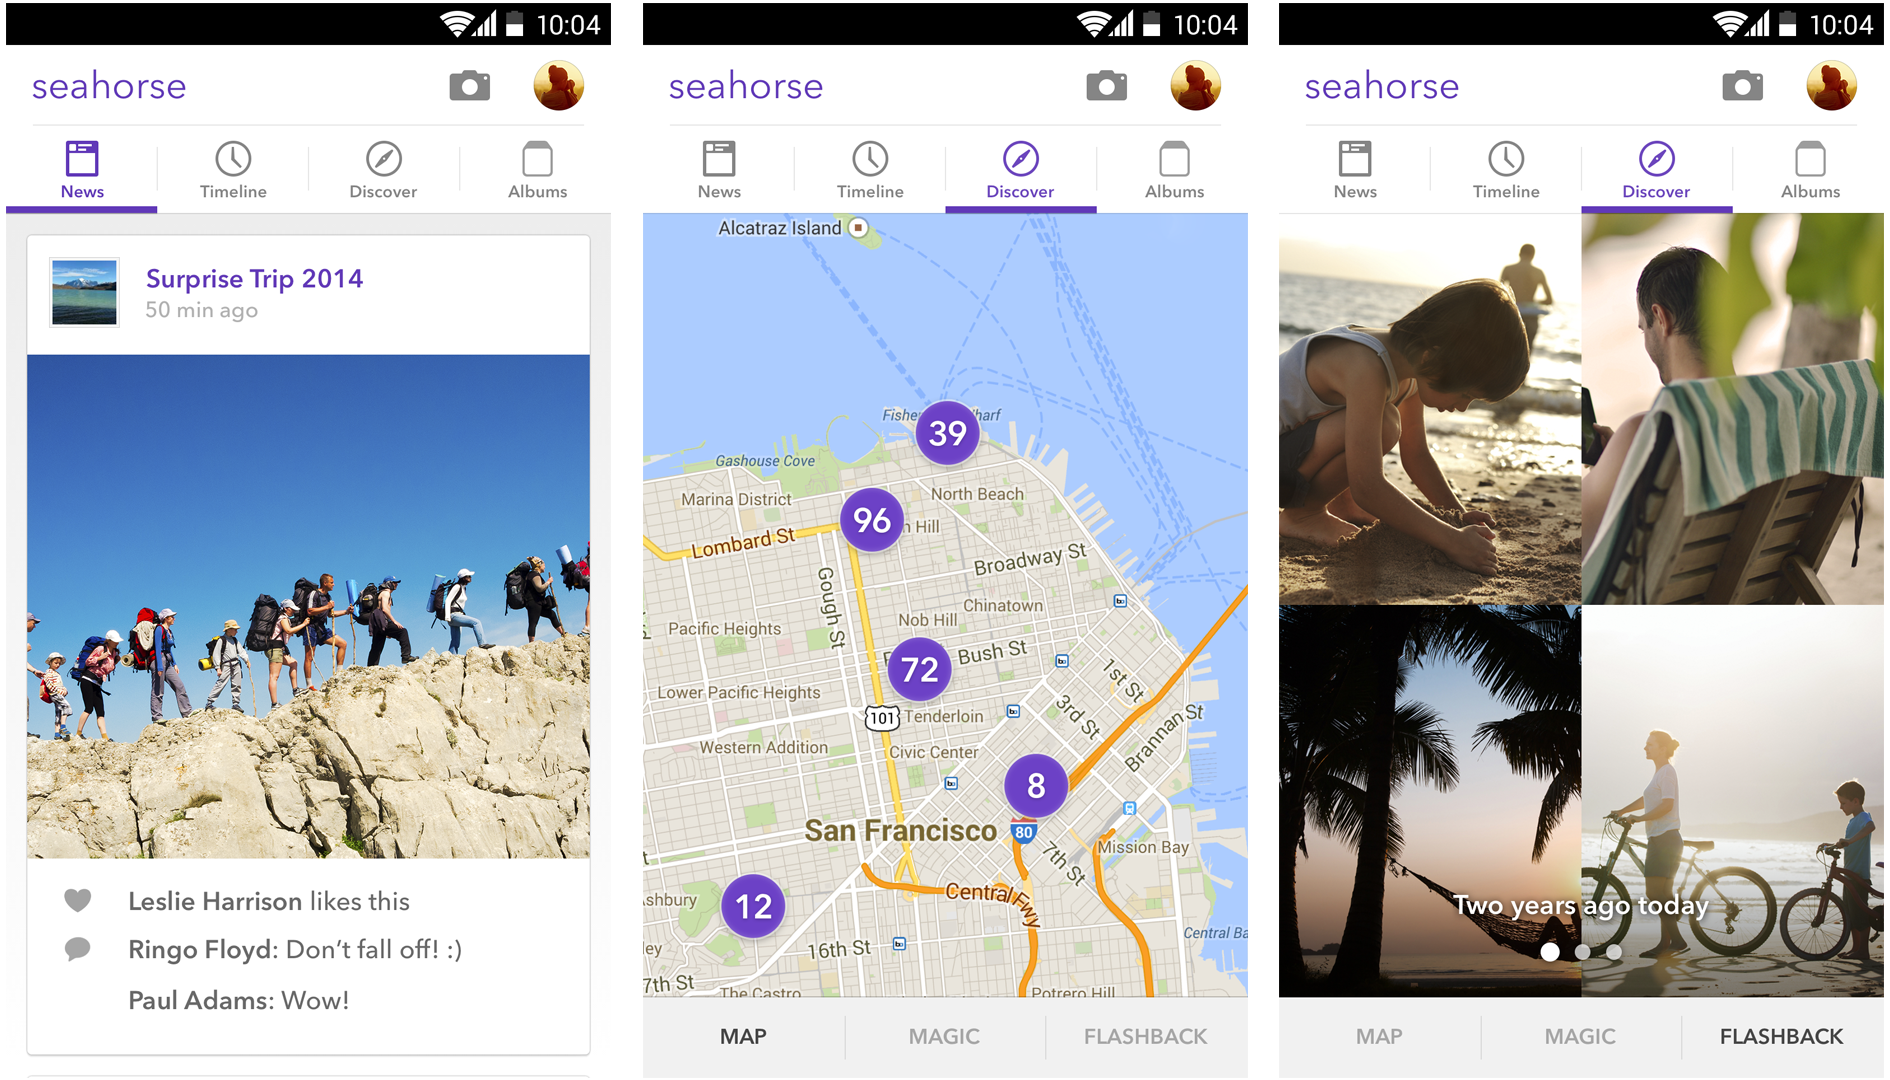
\includegraphics[width=15cm]{Imagenes/seahorse_screenshots}
\caption{Vistas de la aplicaci�n Seahorse. Fuente: Elaboraci�n Propia}
\label{fig:Fig20}
\end{figure}

Las herramientas implementadas son las que m�s se ajustaban a las necesidades y a los recursos con los que cuenta Seahorse, por lo que f�cilmente este conjunto de herramientas puede diferir en relaci�n a las implementaciones que otros desarrolladores har�an en sus aplicaciones.

\section{Implementaci�n de Herramientas de Testing}
\subsection{Robolectric}
Para la implementaci�n de Robolectric es necesario seguir los pasos de instalaci�n que se detallan en su sitio oficial \cite{56}. En Seahorse se usa Gradle para manejar las dependencias, por lo que es necesario agregar esta l�nea a \textit{build.gradle}:
\begin{lstlisting}
dependencies {
  ...
  androidTestCompile 'org.robolectric:robolectric:2.3' 
}
\end{lstlisting}
Para m�s detalles sobre como realizar la instalaci�n con Android Studio, se puede seguir el tutorial que presenta en su blog \cite{57} uno de los desarrolladores de Google.

El test que se llev� a cabo consiste en verificar que el flujo inicial de la aplicaci�n se realice de forma correcta. B�sicamente se testea que el usuario pueda acceder sin problemas a las pantallas de login y de registro. En la figura \ref{fig:Fig21} se muestra el flujo que se someter� a prueba, el cual consta de 3 tareas b�sicas:
\begin{itemize}
\item Abrir Seahorse.

\item Presionar el bot�n que dice \textit{Log In} y mostrar un menu con opciones.

\item Presionar el bot�n que dice \textit{Sign in with email} y llevar al usuario a la vista de Login.
\end{itemize}

\begin{figure}[h!]
\centering
      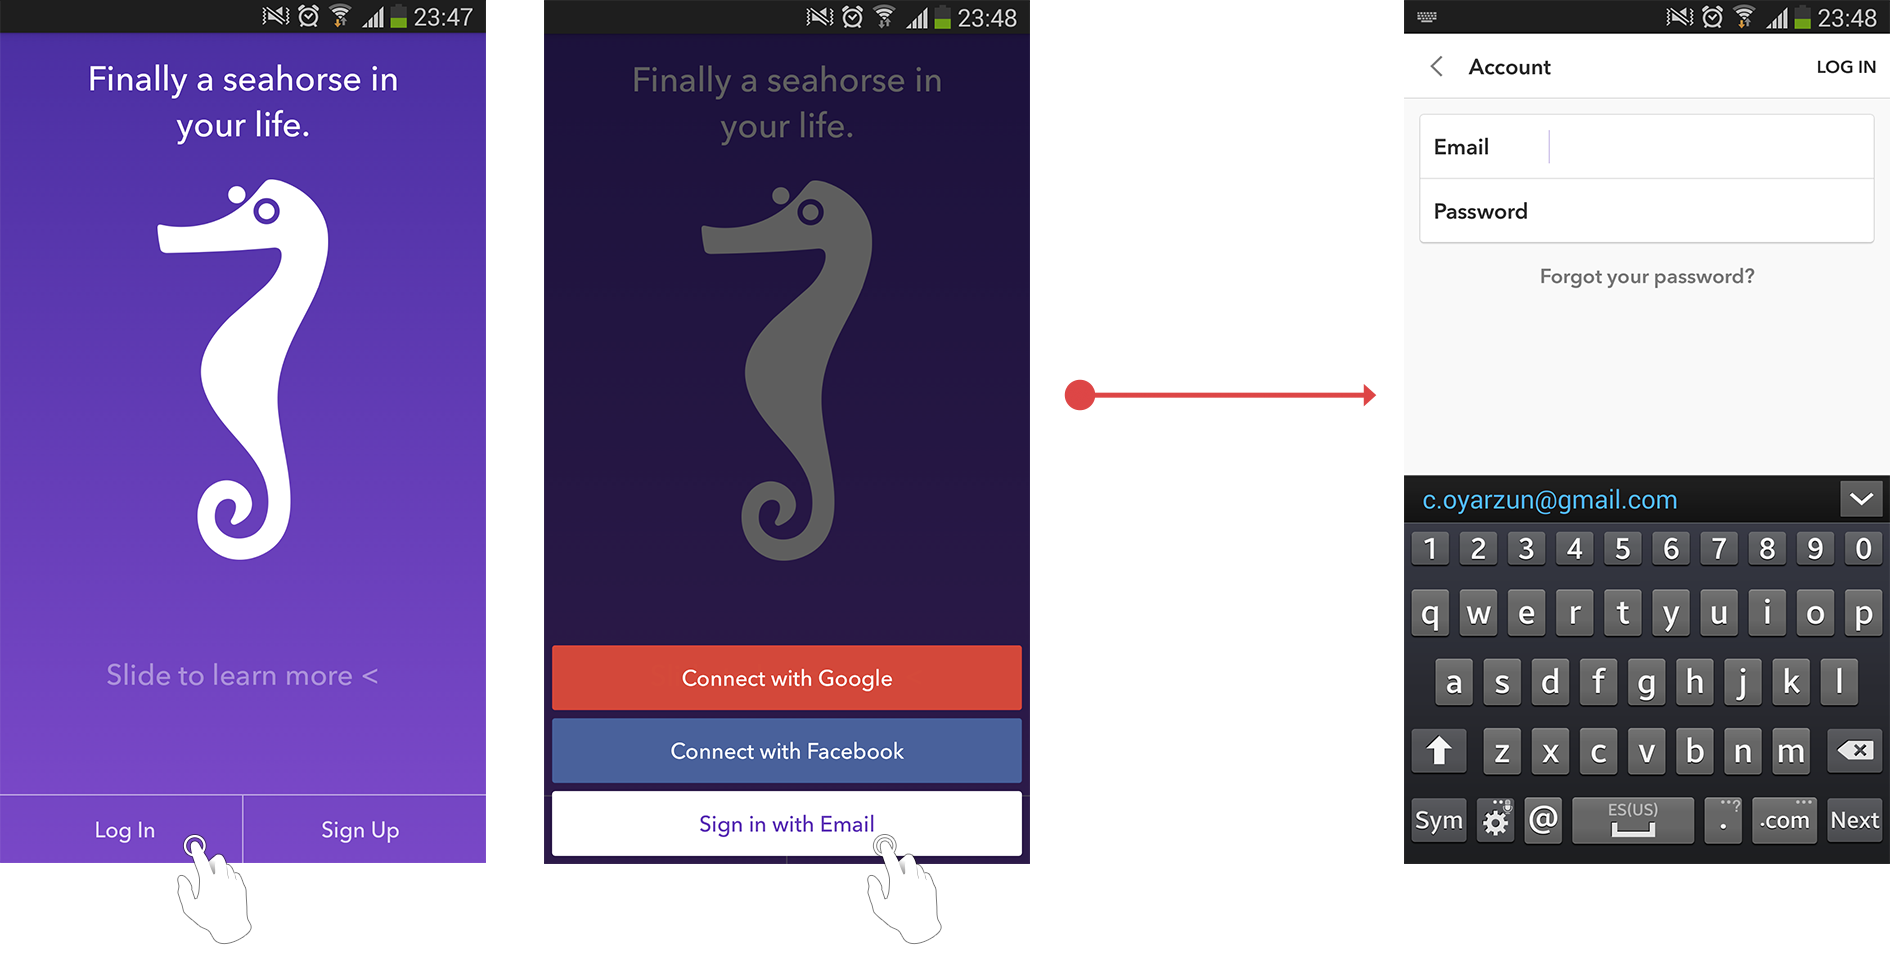
\includegraphics[width=15cm]{Imagenes/seahorse_testing_flujo_login}
\caption{Flujo para acceder a la pantalla de Login en la aplicaci�n Seahorse. En la primera imagen se presiona el bot�n \textit{Log In}, lo cual abre el menu de la segunda imagen, y se presiona el bot�n \textit{Sign in with email}, lo cual abre la vista de Login de la �ltima imagen. Fuente: Elaboraci�n Propia}
\label{fig:Fig21}
\end{figure}

Dentro del proyecto de Seahorse, se cre� una clase en el paquete \textit{co.seahorse.android.test}. En este caso la \textit{Activity} testeada es SeahorseStartActivity y el nombre de la clase que se encarga de realizar el test es SeahorseStartActivityTest. 
\begin{lstlisting}
@RunWith(RobolectricGradleTestRunner.class)
public class SeahorseStartActivityTest {
    private SeahorseStartActivity activity;
    private Button buttonLogin;
    private Button buttonRegister;
    private Button buttonSign;
    @Before
    public void setup() throws Exception {
        activity = Robolectric.buildActivity(SeahorseStartActivity.class).create().start().get();
        buttonLogin = (Button) activity.findViewById(R.id.buttonLogInAccount);
        buttonRegister = (Button) activity.findViewById(R.id.buttonRegisterAccount);
        buttonSign = (Button) activity.findViewById(R.id.buttonSignIn);
    }
\end{lstlisting}
El m�todo \textit{setup()} se encarga de crear la referencia a la \textit{Activity} que se desea testear y obtener los botones que tambi�n ser�n testeados.

Es una buena pr�ctica verificar que ninguno de los elementos obtenidos en el m�todo anterior esten vac�os, por lo que el primer test se encargar� de eso:
\begin{lstlisting}
    @Test
    public void shouldNotBeNull() {
        assertNotNull(activity);
        assertNotNull(buttonLogin);
        assertNotNull(buttonRegister);
        assertNotNull(buttonSign);
    }
\end{lstlisting}

Por �ltimo se realiza el test del flujo que lleva a la pantalla de Login:
\begin{lstlisting}
    @Test
    public void buttonClickShouldStarLoginActivity() throws Exception {
        buttonLogin.performClick();
        buttonSign.performClick();
        Intent intent = Robolectric.shadowOf(activity).peekNextStartedActivity();
        assertEquals(LoginActivity.class.getCanonicalName(), intent.getComponent().getClassName());
    }
    \end{lstlisting}
A trav�s del m�todo \textit{performClick()} es posible simular la l�gica del boton, tal como si un usuario real lo hubiese presionado. Esto se realiza dos veces, ya que se tienen que simular dos clicks a dos botones distintos. El �ltimo de los click es el que abre la pantalla de Login por lo que se verifica que la \textit{Activity} que se inici� corresponda a \textit{LoginActivity}.

Al ejecutar los tests, se genera un reporte en HTML, que se ubica en la raiz del proyecto, en \textit{./build/test-report/index.html}. En este reporte se detallan la cantidad total de test ejecutados y el tiempo que se demoraron, como tambi�n los test que fallaron y la raz�n.

\subsection{Robotium}
Se implement� Robotium, en vez de Espresso, principalmente porque existe mayor documentaci�n y porque cuenta con soporte para gradle de forma oficial, por lo que la integraci�n con Android Studio es menos compleja. Adem�s lleva m�s tiempo de desarrollo y es una herramienta bastante madura.

Para la implementaci�n es necesario agregar la siguiente dependencia al archivo gradle del proyecto:
\begin{lstlisting}
dependencies {
  ...
  androidTestCompile 'com.jayway.android.robotium:robotium-solo:4.3'
}
\end{lstlisting}
El test que se realiz� es similar al realizado a trav�s de Robolectric, aunque ahora de forma instrumental, es decir ejecut�ndolo directamente en el dispositivo. Para ello se ha creado la clase RobotiumTest, la cual consiste en lo siguiente:
\begin{lstlisting}
public class RobotiumTest extends ActivityInstrumentationTestCase2 {
    private Solo solo;

    public RobotiumTest() {
        super(SeahorseStartActivity.class);
    }

    public void setUp() throws Exception {
        super.setUp();
        solo = new Solo(getInstrumentation(), getActivity());
    }

    public void testRobotium()  throws Exception {

        solo.assertCurrentActivity("SeahorseStartActivity Never Loaded", SeahorseStartActivity.class);
        solo.clickOnText(getActivity().getString(R.string.LOGIN));
        solo.waitForText(getActivity().getString(R.string.SIGN_IN_WITH_EMAIL));
        solo.clickOnText(getActivity().getString(R.string.SIGN_IN_WITH_EMAIL));
        solo.assertCurrentActivity("LoginActivity Never Loaded", LoginActivity.class);
        solo.takeScreenshot();
    }
\end{lstlisting}
La clase \textit{Solo} es la principal para desarrollar tests con Robotium. En el m�todo \textit{setup()} se crea una referencia de \textit{Solo} a partir de la \textit{Activity} actual.

En el m�todo \textit{testRobotium()} es donde se lleva a cabo el test. Como se puede ver, todo se realiza a trav�s de la clase \textit{Solo}. Con ella se corrobora en un principio si la \textit{Activity} actual corresponde a \textit{SeahorseStartActivity}, luego se hace un click en el texto que dice ``Log In''. Debido a que existe una animaci�n para mostrar el menu, se recurre al m�todo \textit{waitForText} para esperar que la animaci�n termine y luego presionar este bot�n. Finalmente se presionar el texto ``Sign in with email'' y se comprueba que la nueva \textit{Activity} actual corresponde a \textit{LoginActivity}. Todo este proceso, al ser ejecutado en un dispositivo real, demora 5.69 segundos, lo cu�l no es mucho, pero si se toma en cuenta que dentro de un proyecto se pueden tener una gran cantidad de tests, entonces si puede decirse que es un tiempo considerable. Debido a esto, es importante decidir de forma sabia, que cosas son realmente necesarias testear de forma instrumental.

%\subsection{Espresso} 
%Para la implementaci�n de Espresso, uno de los mayores problemas es que no cuenta oficialmente con soporte para gradle, por lo que se utiliz� la biblioteca Double Espresso \cite{58}, que no cambia en nada el c�digo original y simplemente le agrega este soporte. Las dependencias agregadas a gradle son:
%\begin{lstlisting}
%dependencies {
%  ...
%  androidTestCompile 'com.jakewharton.espresso:espresso:1.1-r3'
%  androidTestCompile 'com.jakewharton.espresso:espresso-support-v4:1.1-r3'
%}
%\end{lstlisting}
%A diferencia de Robolectric, Espresso se especializa en los test relacionados con la interfaz de la aplicaci�n. 
\subsection{Spoon}
....
\subsection{uiautomatorviewer}
Esta es una herramienta de apoyo, que puede servir para personas que est�n involucradas en el desarrollo de un proyecto m�bil, pero que no son desarrolladores. Se puede obtener informaci�n muy detallada sobre el �rbol jer�rquico de vistas y de cada uno de sus elementos. A trav�s de esta informaci�n es posible planear diferentes tipos de tests.\\

En la figura \ref{fig:Fig19} se puede apreciar que a la izquierda se tiene una screenshot de la aplicaci�n, y al lado derecho se muestra el �rbol jer�rquico de vistas de la aplicaci�n. Adem�s el desarrollador puede presionar sobre los elementos del screenshot y obtener informaci�n sobre esa vista, tales como la clase, si la vista tiene habilitado el scroll, si la vista se le puede hacer click, entre otras cosas.

\begin{figure}[h!]
\centering
      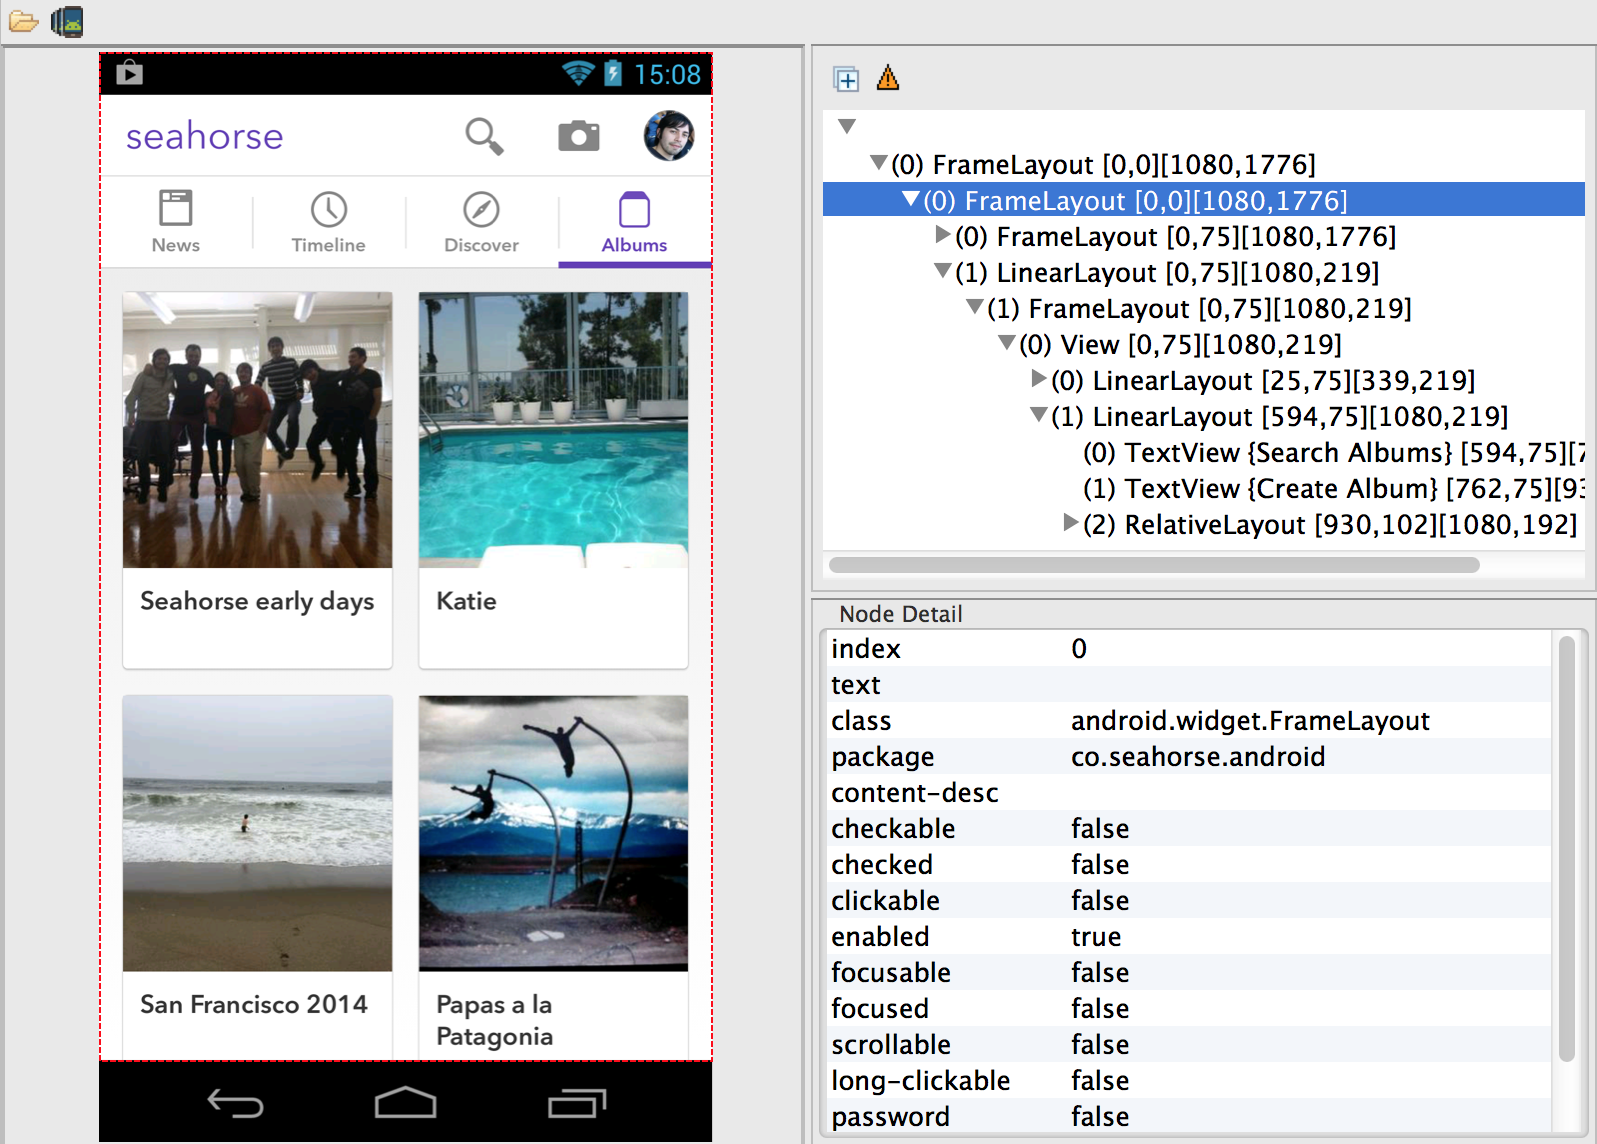
\includegraphics[width=15cm]{Imagenes/testing_uiautomatorview}
\caption{Vista de la herramienta uiautomatorviewer en una aplicaci�n. Fuente: Elaboraci�n Propia}
\label{fig:Fig19}
\end{figure}

\subsection{Monkey}
Esta herramienta es principalmente usada para realizar casos de testing de estr�s. Esto quiere decir que la aplicaci�n es deliberadamente sometida a una gran cantidad de eventos para determinar la estabilidad y el manejo de errores. Los eventos generados consistir�n en acciones que podr�a realizar un usuario normal, como clicks, toques, o gestos, pero un una cantidad muy elevada.\\

Por ejemplo, el siguiente comando enviar� 2000 eventos aleatorios a la aplicaci�n con el nombre de paquete co.seahorse.android:\\

\begin{lstlisting}
adb shell monkey -p co.seahorse.android -v 2000
\end{lstlisting}

\newpage
\section{Implementaci�n de Herramientas de Distribuci�n}
\subsection{HockeyApp}
Antes de HockeyApp, en Seahorse se usaba TestFlight \cite{59}, pero ellos dejaron de dar soporte a Android en Marzo de este a�o \cite{60} ya que fueron comprados por Apple, por lo que fue necesario migrar a otro servicio. HockeyApp cumpl�a con pr�cticamente todas las necesidades que entregaba TestFlight, siendo una de ellas el soporte para  aplicaciones tanto Android como iOS. 

Actualmente se pagan 10 d�lares por el servicio, de forma mensual, lo que corresponde al plan m�s econ�mico ofrecido por HockeyApp, que permite tener hasta 5 aplicaciones distintas en la plataforma, con una cantidad ilimitada de usuarios.

Para distribuir las versiones, la primera vez es necesario agregar informaci�n b�sica como el nombre de la aplicaci�n y el nombre del paquete. Luego se sube el APK de la aplicaci�n y se invita a las personas que se deseen a esta versi�n. Cada vez que se sube una versi�n nueva, es posible notificar a los usuarios que ya cuentan con una versi�n anterior para que la actualicen. Adem�s, es posible invitar a nuevas personas en cualquier momento. 

El desarrollador cuenta con informaci�n b�sica de los testers, como el modelo y dispositivo con el que cuenta, y tambi�n es posible saber si es que ya tienen la �ltima versi�n.

En la figura \ref{fig:Fig22} se puede ver la vista que tiene el desarrollador sobre una versi�n beta de Seahorse. La acciones m�s frecuente est�n en la parte superior, teniendo opciones para subir una nueva versi�n de la misma aplicaci�n, invitar m�s usuarios o cambiar informaci�n b�sica de la aplicaci�n. En la parte inferior es posible ver la lista de todas las �ltimas versiones que se han enviado de esa aplicaci�n, con informaci�n como el peso de la aplicaci�n, cuando fue subida esa actualizaci�n y la cantidad de descargas que se han tenido. En Seahorse no est� implementado el SDK que entrega reporte de crashes, ya que se usa otra herramienta m�s avanzada para ello. Por �ltimo, sobre las acciones m�s frecuente hay un menu que ofrece la opci�n de ver todas las versiones que ha tenido la beta, la lista de usuarios que tienen acceso a la beta y el posible feedback que han entregado cada uno de ellos.
\begin{figure}
\centering
      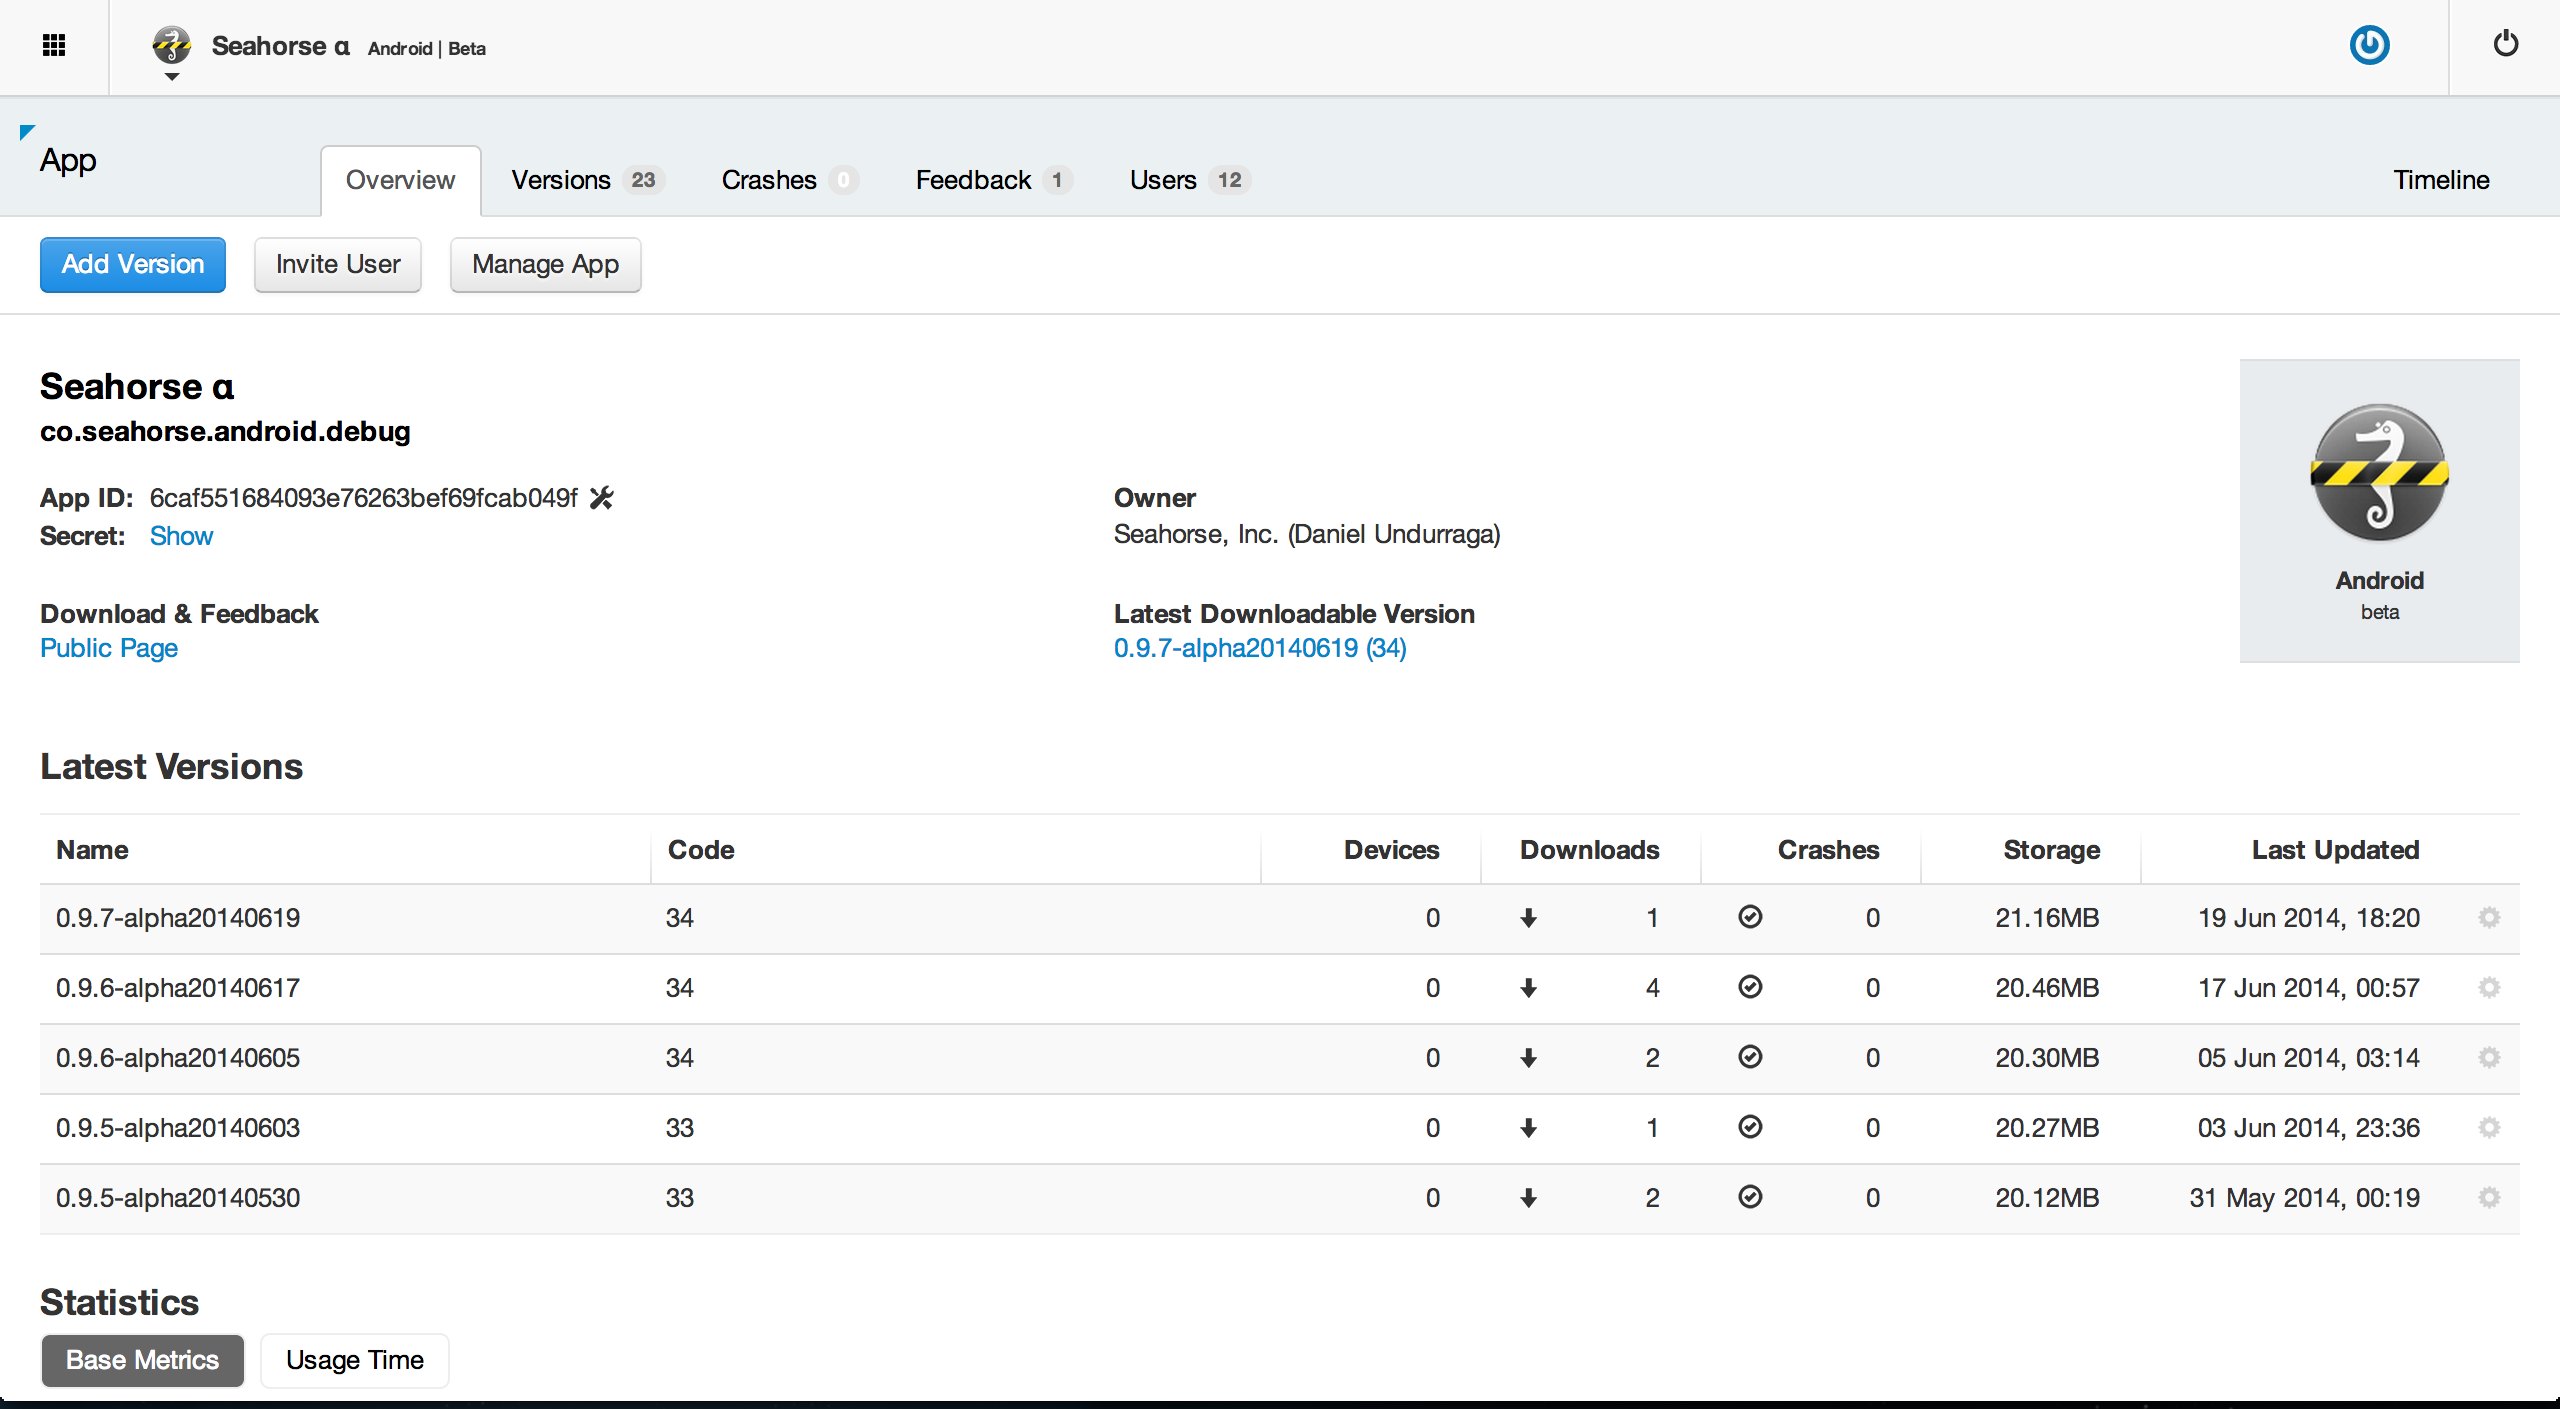
\includegraphics[width=15cm]{Imagenes/distribution_hockeyapp}
\caption{Vista de una aplicaci�n beta de Seahorse en HockeyApp. Fuente: Elaboraci�n Propia}
\label{fig:Fig22}
\end{figure}
%Para su implementaci�n es necesario crearse una cuenta dentro del sitio ....crear la app, subir apk, invitar gente al apk, dps de cada actualizacion aparece la lista de personas para notificarla, en la misma plataforma se puede ver el feedback que dan los usuarios.

\subsection{UserTesting}
UserTesting es la plataforma usada en Seahorse para lanzar versiones beta y recibir feedback de usuarios de prueba a trav�s de videos. Esta herramienta es usada por grandes empresas como Google, Apple, Microsoft, Twitter, Facebook y  Yahoo, para la distribuci�n y testing de versiones de prueba de sitios web, aplicaciones de escritorios y aplicaciones m�biles. El servicio funciona a trav�s de la compra de cr�ditos, en donde por ejemplo, 1000 d�lares otorgan al desarrollador 20 cr�ditos. Cada uno de estos cr�ditos sirve para realizar un test con un usuario, aunque tambi�n es posible realizar un mismo test a m�s de un usuario, pero en definitiva, por cada usuario que realice un test, un cr�dito es consumido. Debido al elevado valor de cada cr�dito, el desarrollador debe tener claro que es lo que quiere testear dentro de la aplicaci�n y cu�les son los resultados que espera.

En Seahorse se usa UserTesting al momento de implementar nuevas caracter�sticas en la aplicaci�n, para ver temas de usabilidad y para corroborar que el usuario entiende de forma intuitiva lo implementado. Adem�s sirve para encontrar posibles errores en otros dispositivos, ya que debido a la fragmentaci�n existente en Android es pr�cticamente imposible saber como una aplicaci�n se ve en cada uno de los dispositivos existentes.

Para la creaci�n de un test los pasos son los siguientes:
\begin{itemize}
\item Seleccionar si la aplicaci�n m�vil es de Android o iOS

\item Agregar instrucciones de como instalar la aplicaci�n y una breve descripci�n para que el usuario tenga una idea de lo que va a testear.

\item Agregar una serie de tareas que el usuario debe ir realizando. Tambi�n se pueden incluir preguntas durante el proceso, para saber si la tarea solicitada fue complicada, o simplemente para saber que piensa el usuario sobre esa tarea.

\item Agregar un cuestionario final con preguntas m�s generales sobre la aplicaci�n y el proceso completo.

\item Por �ltimo es posible solicitar algunas caracter�sticas demogr�ficas como el rango de edad, el pa�s, el g�nero, la experiencia con aplicaciones m�viles, y otras restricciones como versi�n de Android mayor a 4.0, o que el usuario cuente con fotos en su galeria.
\end{itemize}

Cuando en Seahorse se agreg� el registro de usuarios a trav�s de Facebook y de Google+, se llevo a cabo la distribuci�n y testing a trav�s de esta plataforma. Esto permiti� corroborar que esta nueva caracter�stica, al igual que otras, funcionaban correctamente. Fue necesario hacer en total unos 8 tests, ya que en cada iteraci�n se usaban 4 cr�ditos, dos para comprobar que el registro a trav�s de Facebook funcionaba bien, y otros 2 para comprobar lo mismo, pero a trav�s de Google+. Los tests a trav�s de Facebook funcionaron correctamente, pero con Google+ existieron dificultades, ya que uno de los usuarios no pudo realizar el registro. Debido a esto, despu�s de realizar algunas correcciones se llevaron a cabo nuevos tests, con los que se obtuvieron resultados positivos. Tal como se mencion� antes, es necesario aprovechar cada uno de los tests, por lo que adem�s de testear el registro de los usuarios, tambi�n se solicitaron otras tareas, como importar albums de otras plataformas, sincronizar la c�mara del dispositivo con Seahorse, invitar a otros usuarios a la aplicaci�n, entre otras.

Cada uno de los videos entreg� informaci�n valiosa sobre la usabilidad dentro de la aplicaci�n, y permiti� verificar la UI en 8 dispositivos distintos, algunos con una pantalla muy peque�a. Los videos duran entre 15 y 20 minutos, y el usuario va relatando todo el proceso, desde la instalaci�n de la aplicaci�n, hasta el cuestionario final.
\newpage
\section{Implementaci�n de Herramientas de Reportes de Crashes}
\subsection{Crittercism}
Crittercism a sido la plataforma escogida para la recepci�n de crashes, principalmente por el nivel de detalle presente en sus reportes. Adem�s el valor que se paga mensualmente es bastante accesible para cualquier empresa del rubro. Actualmente dentro de Seahorse, se pagan 24 d�lares por este servicio, lo que da acceso a reportes muy detallados que permiten reparar de forma r�pida cada crash. 

Crittercism ha permitido disminuir la tasa de crashes y ofrece variadas estad�sticas para ver informaci�n como los dispositivos en los que existen m�s crashes, el sistema operaritivo en que ocurren m�s crashes o la versi�n en la que ocurrieron m�s crashes. Despu�s del lanzamiento de cada actualizaci�n se reparan una gran cantidad de bugs, pero aparecen nuevos crashes, lo que es inherente al proceso de desarrollo de software, ya que se incluye nuevo c�digo, pero con esta herramienta es posible contar con informaci�n muy detallada, facilitando en gran medida la tarea de los desarrolladores.

La instalaci�n es bastante simple \cite{31}. Existen dos formas en que se puede incluir el SDK de Crittercism, la primera es descarg�ndolo desde el sitio web e incluyendolo al proyecto, la segunda es agregando la dependencia al archivo gradle del proyecto de la siguiente forma:
\begin{lstlisting}
compile 'com.crittercism:crittercism-android-agent:+'
\end{lstlisting}
Luego se deben agregar los siguientes permisos en el archivo Android Manifest del proyecto: 
\begin{lstlisting}
<uses-permission android:name="android.permission.INTERNET"/>
<uses-permission android:name="android.permission.READ_LOGS"/>
<uses-permission android:name="android.permission.ACCESS_NETWORK_STATE"/>
<uses-permission android:name="android.permission.GET_TASKS"/>
\end{lstlisting}
El primer permiso es necesario para poder acceder a Internet y poder enviar los reportes. El segundo es necesario para poder obtener la informaci�n de los stack trace del usuario, y ahi saber en que l�nea de c�digo ha ocurrido el error. El tercero es para obtener informaci�n sobre el estado de la red, por ejemplo, para saber si el usuario est� conectado a Wi-Fi o a trav�s de un carrier. El �ltimo permiso sirve para acceder a la informaci�n de las �ltimas dos \textit{Activities} ejecutadas, lo que permite saber en que pantalla ocurri� el crash.

Una vez que los permisos ya est�n entregados, se debe inicializar Crittercism. Esto se hace �nicamente una vez por aplicaci�n, por lo que se debe hacer en la primera \textit{Activity} que se ejecuta dentro de la aplicaci�n. Para iniciar Crittercism se escribe la siguiente l�nea en el onCreate:
\begin{lstlisting}
Crittercism.initialize(getApplicationContext(), "CRITTERCISM_APP_ID");
\end{lstlisting}

Ahora ya est�n implementadas las caracter�sticas b�sicas, y comenzar�n a llegar los reportes al sitio web de Crittercism. Tambi�n es posible agregar a otros desarrolladores al servicio, para que tengan acceso a la misma informaci�n y que todo el equipo reciba los reportes de crashes al correo.

La documentaci�n con la que cuenta es excelente para entender los alcances y todas las cosas que se pueden hacer a trav�s de Crittercism. Por ejemplo, es posible recibir las excepciones que ocurren dentro de la aplicaci�n. Esto se realiza agregando las siguientes l�neas en la excepci�n que se desea recibir:
\begin{lstlisting}
try {
    throw new Exception("Aqu� ocurre una excepci�n");
} catch (Exception exception) {
    //De esta forma se captura y se env�a a Crittercism
    Crittercism.logHandledException(exception);
}
\end{lstlisting}

A trav�s de los gr�ficos de la figura \ref{fig:Fig23} es posible dimensionar la utilidad de contar con una herramienta como Crittercism. El gr�fico de la izquierda indica la cantidad de reportes de crashes recibidos por distintas versiones de la aplicaci�n durante el mes de Enero. El gr�fico de la derecha indica la cantidad de usuarios que han sido afectados por al menos un crash durante ese mismo periodo. A trav�s de estos gr�ficos es posible ver que la versi�n 0.8.8 de color amarillo, fue lanzada el d�a 9 de Enero y r�pidamente comenzaron a llegar una gran cantidad de reportes de crashes, alcanzando la cifra de 173 crashes y afectando a m�s de 100 usuarios. Debido a ello, al d�a siguiente se lanz� la versi�n 0.8.8.1 de color verde, la cu�l se encarg� de arreglar el error introducido en la versi�n previa y reduciendo este n�mero en gran medida, con s�lo 35 crashes y afectando a 20 usuarios. Si no se hubiera contado con una herramienta que entregue los reportes de crashes en tiempo real, probablemente habr�an transcurrido m�s d�as con el mismo problema, afectando a muchos m�s usuarios. 
\begin{figure}
\centering
      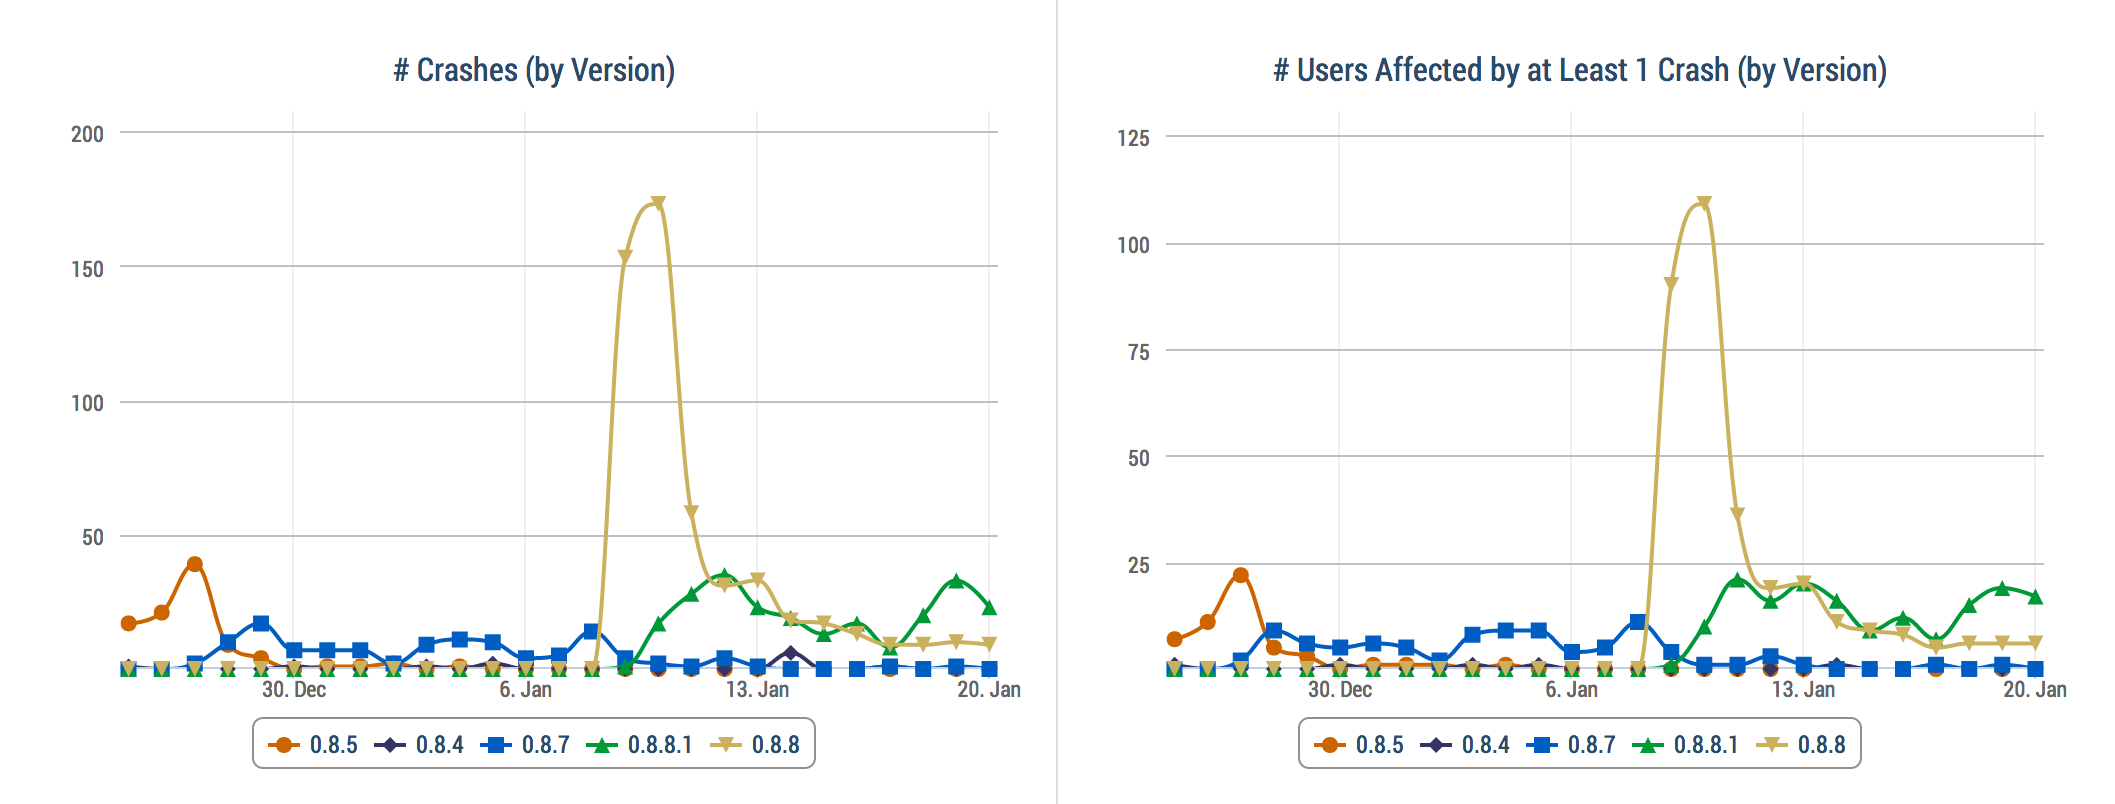
\includegraphics[width=16cm]{Imagenes/crash_report_crittercism_graphs}
\caption{Gr�ficos que entrega Crittercism sobre cantidad de crashes y usuarios afectados en un periodo de un mes. Fuente: Elaboraci�n Propia}
\label{fig:Fig23}
\end{figure}

\subsection{Google Analytics}
Google Analytics ha sido implementada, aunque no por sus reportes de crashes, sino que para el tracking de eventos y performance.
Para su implementaci�n es necesario descarga desde el sitio de Google Analytics \cite{33} la versi�n 3 de su SDK. Una vez descargado el SDK, es necesario incluirlo al proyecto y dar los siguientes permisos en el archivo Android Manifest:
\begin{lstlisting}
<uses-permission android:name="android.permission.INTERNET"/>
<uses-permission android:name="android.permission.ACCESS_NETWORK_STATE"/>
\end{lstlisting}
Para implementarlo a trav�s de c�digo es necesario agregar estas l�neas en cada una de las \textit{Activities} de las cu�les se desee obtener informaci�n:
\begin{lstlisting}
@Override
  public void onStart() {
    super.onStart();
    ... // El resto del c�digo de onStart()
    EasyTracker.getInstance(this).activityStart(this);  // Agregar este m�todo
  }

  @Override
  public void onStop() {
    super.onStop();
    ... // El resto del c�digo de onStop()
    EasyTracker.getInstance(this).activityStop(this);  // Agregar este m�todo
  }
\end{lstlisting}
% ---------------------------------------------------------------------------------------------------------------
% Cap�tulo 5: Conclusiones y Trabajo Futuro
% ---------------------------------------------------------------------------------------------------------------
\chapter{Conclusiones}
\label{ch:conc}
A trav�s de este trabajo, se han estudiado y comparado diversas herramientas que ayudan a mejorar la calidad de las aplicaciones desarrolladas para Android. Esto se ha llevado a cabo clasificando las distintas herramientas en tres categorias principales: Testing, Distribuci�n de versiones y Reportes de Crashes.  

En cada una de las categor�as se ha realizado un an�lisis comparativo, a trav�s del cual se han obtenido las ventajas y desventajas de cada una de las herramientas. En algunos casos ha sido necesario subdividir las categor�as para que las comparaciones arrojen resultados m�s �tiles. Esto permite que los desarrolladores cuenten con informaci�n relevante que les ayude a tomar mejores decisiones al momento de tener que implementar una de estas herramientas. 

En base a las caracter�sticas de cada herramienta, se han implementado algunas de estas en una aplicaci�n que est� disponible en la tienda oficial de Google. Cabe mencionar que las herramientas implemetadas se ajustaban m�s a las necesidades de \textit{Seahorse}, ya que es posible que otros desarrolladores, en base a las ventajas y desventajas presentadas, implementen otro conjunto de herramientas, que se ajuste m�s al contexto en que trabajan.

...



\section{Trabajo Futuro}

% ---------------------------------------------------------------------------------------------------------------

\appendix
% Ap�ndice A: 
% ---------------------------------------------------------------------------------------------------------------
\chapter{Ap�ndice A}
\label{ch:apeA}

\section{Secci�n Ap�ndice}
\label{sec:SecApe}

% ---------------------------------------------------------------------------------------------------------------
% ---------------------------------------------------------------------------------------------------------------
\singlespacing
\bibliographystyle{plain}
\bibliography{manual} %Use Mendeley Tool or automatic creation (http://mendeley.com)
% ---------------------------------------------------------------------------------------------------------------
\end{document} 